% ***************************************************** %
%                   1st Draft Template                  %
% ***************************************************** %
%For 1st draft to the collaboration
\documentclass[12pt,twoside,letterpaper,doublespace]{article}

\topmargin -0.25cm
\textwidth 15.5cm
\textheight 22cm
\oddsidemargin 0.5cm
\evensidemargin 0.5cm

\usepackage{graphicx}% Include figure files
\usepackage{dcolumn}% Align table columns on decimal point
\usepackage{bm}% bold math
\usepackage{lineno}
\usepackage{setspace}
\usepackage{xspace}
\usepackage{subfigure}
\usepackage{multirow}  % multirows in tables
\usepackage{multicol}


\begin{document}

%define my commands here
\def\sla#1{\rlap{\kern .15em /}#1}
\newcommand{\ppbar}{$p\bar{p}$\xspace}
\newcommand{\met}{\mbox{$\sla{E}_T$}\xspace}
\newcommand{\pt}{\mbox{$p_T$}\xspace}
\newcommand{\Ht}{\mbox{$H_T$}\xspace}
\newcommand{\et}{\mbox{$E_T$}\xspace}
\newcommand{\eoverp}{\mbox{$E/p$}\xspace}
\newcommand{\isoetcorr}{\mbox {$E_ {T}^{Iso(corr)}$\xspace }}
\newcommand{\phojets}{\mbox{$\gamma$ + jets}\xspace}
\newcommand{\phoonejet}{\mbox{$\gamma$ + $\geq$1 jet}\xspace}
\newcommand{\photwojet}{\mbox{$\gamma$ + $\geq$2 jet}\xspace}
\newcommand{\phojetsmet}{\mbox{\phojets + \met}\xspace}
\newcommand{\metCorr}{$\sla{E}_T^{corr}$\xspace}
\newcommand{\figScale}{0.35}
\newcommand{\MC}{Monte Carlo}
\newcommand{\pythiaText}{\textsc{pythia}\xspace}
\newcommand{\pizero}{$\pi^{0}$}
\newcommand{\alphas}{$\alpha_s$\xspace}

%%%%%%%%%%%%%%%%%%%%%%%%%%%%%%%%%%%%%%%%%%%%%%%
% Toggle double spacing and line numbering
% Won't work with the PRD revtex4 !
\pagewiselinenumbers
%\doublespace
%%%%%%%%%%%%%%%%%%%%%%%%%%%%%%%%%%%%%%%%%%%%%%%

%uncomment for the PRD
\title{Search for Anomalous Production of Photon + Jets + Missing Transverse Energy in \ppbar Collisions at $\sqrt{s}=1.96$~TeV Using the CDF II Detector}
% \affiliation{Institute of Physics, Academia Sinica, Taipei, Taiwan 11529, Republic of China}
\affiliation{Argonne National Laboratory, Argonne, Illinois 60439, USA}
\affiliation{University of Athens, 157 71 Athens, Greece}
\affiliation{Institut de Fisica d'Altes Energies, ICREA, Universitat Autonoma de Barcelona, E-08193, Bellaterra (Barcelona), Spain}
\affiliation{Baylor University, Waco, Texas 76798, USA}
\affiliation{Istituto Nazionale di Fisica Nucleare Bologna, $^{aa}$University of Bologna, I-40127 Bologna, Italy}
\affiliation{University of California, Davis, Davis, California 95616, USA}
\affiliation{University of California, Los Angeles, Los Angeles, California 90024, USA}
\affiliation{Instituto de Fisica de Cantabria, CSIC-University of Cantabria, 39005 Santander, Spain}
\affiliation{Carnegie Mellon University, Pittsburgh, Pennsylvania 15213, USA}
\affiliation{Enrico Fermi Institute, University of Chicago, Chicago, Illinois 60637, USA}
\affiliation{Comenius University, 842 48 Bratislava, Slovakia; Institute of Experimental Physics, 040 01 Kosice, Slovakia}
\affiliation{Joint Institute for Nuclear Research, RU-141980 Dubna, Russia}
\affiliation{Duke University, Durham, North Carolina 27708, USA}
\affiliation{Fermi National Accelerator Laboratory, Batavia, Illinois 60510, USA}
\affiliation{University of Florida, Gainesville, Florida 32611, USA}
\affiliation{Laboratori Nazionali di Frascati, Istituto Nazionale di Fisica Nucleare, I-00044 Frascati, Italy}
\affiliation{University of Geneva, CH-1211 Geneva 4, Switzerland}
\affiliation{Glasgow University, Glasgow G12 8QQ, United Kingdom}
\affiliation{Harvard University, Cambridge, Massachusetts 02138, USA}
\affiliation{Division of High Energy Physics, Department of Physics, University of Helsinki and Helsinki Institute of Physics, FIN-00014, Helsinki, Finland}
\affiliation{University of Illinois, Urbana, Illinois 61801, USA}
\affiliation{The Johns Hopkins University, Baltimore, Maryland 21218, USA}
\affiliation{Institut f\"{u}r Experimentelle Kernphysik, Karlsruhe Institute of Technology, D-76131 Karlsruhe, Germany}
\affiliation{Center for High Energy Physics: Kyungpook National University, Daegu 702-701, Korea; Seoul National University, Seoul 151-742, Korea; Sungkyunkwan University, Suwon 440-746, Korea; Korea Institute of Science and Technology Information, Daejeon 305-806, Korea; Chonnam National University, Gwangju 500-757, Korea; Chonbuk National University, Jeonju 561-756, Korea}
\affiliation{Ernest Orlando Lawrence Berkeley National Laboratory, Berkeley, California 94720, USA}
\affiliation{University of Liverpool, Liverpool L69 7ZE, United Kingdom}
\affiliation{University College London, London WC1E 6BT, United Kingdom}
\affiliation{Centro de Investigaciones Energeticas Medioambientales y Tecnologicas, E-28040 Madrid, Spain}
\affiliation{Massachusetts Institute of Technology, Cambridge, Massachusetts 02139, USA}
\affiliation{Institute of Particle Physics: McGill University, Montr\'{e}al, Qu\'{e}bec, Canada H3A~2T8; Simon Fraser University, Burnaby, British Columbia, Canada V5A~1S6; University of Toronto, Toronto, Ontario, Canada M5S~1A7; and TRIUMF, Vancouver, British Columbia, Canada V6T~2A3}
\affiliation{University of Michigan, Ann Arbor, Michigan 48109, USA}
\affiliation{Michigan State University, East Lansing, Michigan 48824, USA}
\affiliation{Institution for Theoretical and Experimental Physics, ITEP, Moscow 117259, Russia}
\affiliation{University of New Mexico, Albuquerque, New Mexico 87131, USA}
\affiliation{Northwestern University, Evanston, Illinois 60208, USA}
\affiliation{The Ohio State University, Columbus, Ohio 43210, USA}
\affiliation{Okayama University, Okayama 700-8530, Japan}
\affiliation{Osaka City University, Osaka 588, Japan}
\affiliation{University of Oxford, Oxford OX1 3RH, United Kingdom}
\affiliation{Istituto Nazionale di Fisica Nucleare, Sezione di Padova-Trento, $^{bb}$University of Padova, I-35131 Padova, Italy}
\affiliation{LPNHE, Universite Pierre et Marie Curie/IN2P3-CNRS, UMR7585, Paris, F-75252 France}
\affiliation{University of Pennsylvania, Philadelphia, Pennsylvania 19104, USA}
\affiliation{Istituto Nazionale di Fisica Nucleare Pisa, $^{cc}$University of Pisa, $^{dd}$University of Siena and $^{ee}$Scuola Normale Superiore, I-56127 Pisa, Italy}
\affiliation{University of Pittsburgh, Pittsburgh, Pennsylvania 15260, USA}
\affiliation{Purdue University, West Lafayette, Indiana 47907, USA}
\affiliation{University of Rochester, Rochester, New York 14627, USA}
\affiliation{The Rockefeller University, New York, New York 10065, USA}
\affiliation{Istituto Nazionale di Fisica Nucleare, Sezione di Roma 1, $^{ff}$Sapienza Universit\`{a} di Roma, I-00185 Roma, Italy}

\affiliation{Rutgers University, Piscataway, New Jersey 08855, USA}
\affiliation{Texas A\&M University, College Station, Texas 77843, USA}
\affiliation{Istituto Nazionale di Fisica Nucleare Trieste/Udine, I-34100 Trieste, $^{gg}$University of Udine, I-33100 Udine, Italy}
\affiliation{University of Tsukuba, Tsukuba, Ibaraki 305, Japan}
\affiliation{Tufts University, Medford, Massachusetts 02155, USA}
\affiliation{University of Virginia, Charlottesville, VA  22906, USA}
\affiliation{Waseda University, Tokyo 169, Japan}
\affiliation{Wayne State University, Detroit, Michigan 48201, USA}
\affiliation{University of Wisconsin, Madison, Wisconsin 53706, USA}
\affiliation{Yale University, New Haven, Connecticut 06520, USA}
\author{T.~Aaltonen}
\affiliation{Division of High Energy Physics, Department of Physics, University of Helsinki and Helsinki Institute of Physics, FIN-00014, Helsinki, Finland}
\author{B.~\'{A}lvarez~Gonz\'{a}lez$^w$}
\affiliation{Instituto de Fisica de Cantabria, CSIC-University of Cantabria, 39005 Santander, Spain}
\author{S.~Amerio}
\affiliation{Istituto Nazionale di Fisica Nucleare, Sezione di Padova-Trento, $^{bb}$University of Padova, I-35131 Padova, Italy}

\author{D.~Amidei}
\affiliation{University of Michigan, Ann Arbor, Michigan 48109, USA}
\author{A.~Anastassov}
\affiliation{Northwestern University, Evanston, Illinois 60208, USA}
\author{A.~Annovi}
\affiliation{Laboratori Nazionali di Frascati, Istituto Nazionale di Fisica Nucleare, I-00044 Frascati, Italy}
\author{J.~Antos}
\affiliation{Comenius University, 842 48 Bratislava, Slovakia; Institute of Experimental Physics, 040 01 Kosice, Slovakia}
\author{G.~Apollinari}
\affiliation{Fermi National Accelerator Laboratory, Batavia, Illinois 60510, USA}
\author{J.A.~Appel}
\affiliation{Fermi National Accelerator Laboratory, Batavia, Illinois 60510, USA}
\author{A.~Apresyan}
\affiliation{Purdue University, West Lafayette, Indiana 47907, USA}
\author{T.~Arisawa}
\affiliation{Waseda University, Tokyo 169, Japan}
\author{A.~Artikov}
\affiliation{Joint Institute for Nuclear Research, RU-141980 Dubna, Russia}
\author{J.~Asaadi}
\affiliation{Texas A\&M University, College Station, Texas 77843, USA}
\author{W.~Ashmanskas}
\affiliation{Fermi National Accelerator Laboratory, Batavia, Illinois 60510, USA}
\author{B.~Auerbach}
\affiliation{Yale University, New Haven, Connecticut 06520, USA}
\author{A.~Aurisano}
\affiliation{Texas A\&M University, College Station, Texas 77843, USA}
\author{F.~Azfar}
\affiliation{University of Oxford, Oxford OX1 3RH, United Kingdom}
\author{W.~Badgett}
\affiliation{Fermi National Accelerator Laboratory, Batavia, Illinois 60510, USA}
\author{A.~Barbaro-Galtieri}
\affiliation{Ernest Orlando Lawrence Berkeley National Laboratory, Berkeley, California 94720, USA}
\author{V.E.~Barnes}
\affiliation{Purdue University, West Lafayette, Indiana 47907, USA}
\author{B.A.~Barnett}
\affiliation{The Johns Hopkins University, Baltimore, Maryland 21218, USA}
\author{P.~Barria$^{dd}$}
\affiliation{Istituto Nazionale di Fisica Nucleare Pisa, $^{cc}$University of Pisa, $^{dd}$University of
Siena and $^{ee}$Scuola Normale Superiore, I-56127 Pisa, Italy}
\author{P.~Bartos}
\affiliation{Comenius University, 842 48 Bratislava, Slovakia; Institute of Experimental Physics, 040 01 Kosice, Slovakia}
\author{M.~Bauce$^{bb}$}
\affiliation{Istituto Nazionale di Fisica Nucleare, Sezione di Padova-Trento, $^{bb}$University of Padova, I-35131 Padova, Italy}
\author{G.~Bauer}
\affiliation{Massachusetts Institute of Technology, Cambridge, Massachusetts  02139, USA}
\author{F.~Bedeschi}
\affiliation{Istituto Nazionale di Fisica Nucleare Pisa, $^{cc}$University of Pisa, $^{dd}$University of Siena and $^{ee}$Scuola Normale Superiore, I-56127 Pisa, Italy}

\author{D.~Beecher}
\affiliation{University College London, London WC1E 6BT, United Kingdom}
\author{S.~Behari}
\affiliation{The Johns Hopkins University, Baltimore, Maryland 21218, USA}
\author{G.~Bellettini$^{cc}$}
\affiliation{Istituto Nazionale di Fisica Nucleare Pisa, $^{cc}$University of Pisa, $^{dd}$University of Siena and $^{ee}$Scuola Normale Superiore, I-56127 Pisa, Italy}

\author{J.~Bellinger}
\affiliation{University of Wisconsin, Madison, Wisconsin 53706, USA}
\author{D.~Benjamin}
\affiliation{Duke University, Durham, North Carolina 27708, USA}
\author{A.~Beretvas}
\affiliation{Fermi National Accelerator Laboratory, Batavia, Illinois 60510, USA}
\author{A.~Bhatti}
\affiliation{The Rockefeller University, New York, New York 10065, USA}
\author{M.~Binkley\footnote{Deceased}}
\affiliation{Fermi National Accelerator Laboratory, Batavia, Illinois 60510, USA}
\author{D.~Bisello$^{bb}$}
\affiliation{Istituto Nazionale di Fisica Nucleare, Sezione di Padova-Trento, $^{bb}$University of Padova, I-35131 Padova, Italy}

\author{I.~Bizjak$^{hh}$}
\affiliation{University College London, London WC1E 6BT, United Kingdom}
\author{K.R.~Bland}
\affiliation{Baylor University, Waco, Texas 76798, USA}
\author{B.~Blumenfeld}
\affiliation{The Johns Hopkins University, Baltimore, Maryland 21218, USA}
\author{A.~Bocci}
\affiliation{Duke University, Durham, North Carolina 27708, USA}
\author{A.~Bodek}
\affiliation{University of Rochester, Rochester, New York 14627, USA}
\author{D.~Bortoletto}
\affiliation{Purdue University, West Lafayette, Indiana 47907, USA}
\author{J.~Boudreau}
\affiliation{University of Pittsburgh, Pittsburgh, Pennsylvania 15260, USA}
\author{A.~Boveia}
\affiliation{Enrico Fermi Institute, University of Chicago, Chicago, Illinois 60637, USA}
\author{B.~Brau$^a$}
\affiliation{Fermi National Accelerator Laboratory, Batavia, Illinois 60510, USA}
\author{L.~Brigliadori$^{aa}$}
\affiliation{Istituto Nazionale di Fisica Nucleare Bologna, $^{aa}$University of Bologna, I-40127 Bologna, Italy}
\author{A.~Brisuda}
\affiliation{Comenius University, 842 48 Bratislava, Slovakia; Institute of Experimental Physics, 040 01 Kosice, Slovakia}
\author{C.~Bromberg}
\affiliation{Michigan State University, East Lansing, Michigan 48824, USA}
\author{E.~Brucken}
\affiliation{Division of High Energy Physics, Department of Physics, University of Helsinki and Helsinki Institute of Physics, FIN-00014, Helsinki, Finland}
\author{M.~Bucciantonio$^{cc}$}
\affiliation{Istituto Nazionale di Fisica Nucleare Pisa, $^{cc}$University of Pisa, $^{dd}$University of Siena and $^{ee}$Scuola Normale Superiore, I-56127 Pisa, Italy}
\author{J.~Budagov}
\affiliation{Joint Institute for Nuclear Research, RU-141980 Dubna, Russia}
\author{H.S.~Budd}
\affiliation{University of Rochester, Rochester, New York 14627, USA}
\author{S.~Budd}
\affiliation{University of Illinois, Urbana, Illinois 61801, USA}
\author{K.~Burkett}
\affiliation{Fermi National Accelerator Laboratory, Batavia, Illinois 60510, USA}
\author{G.~Busetto$^{bb}$}
\affiliation{Istituto Nazionale di Fisica Nucleare, Sezione di Padova-Trento, $^{bb}$University of Padova, I-35131 Padova, Italy}

\author{P.~Bussey}
\affiliation{Glasgow University, Glasgow G12 8QQ, United Kingdom}
\author{A.~Buzatu}
\affiliation{Institute of Particle Physics: McGill University, Montr\'{e}al, Qu\'{e}bec, Canada H3A~2T8; Simon Fraser
University, Burnaby, British Columbia, Canada V5A~1S6; University of Toronto, Toronto, Ontario, Canada M5S~1A7; and TRIUMF, Vancouver, British Columbia, Canada V6T~2A3}
\author{C.~Calancha}
\affiliation{Centro de Investigaciones Energeticas Medioambientales y Tecnologicas, E-28040 Madrid, Spain}
\author{S.~Camarda}
\affiliation{Institut de Fisica d'Altes Energies, ICREA, Universitat Autonoma de Barcelona, E-08193, Bellaterra (Barcelona), Spain}
\author{M.~Campanelli}
\affiliation{Michigan State University, East Lansing, Michigan 48824, USA}
\author{M.~Campbell}
\affiliation{University of Michigan, Ann Arbor, Michigan 48109, USA}
\author{F.~Canelli$^{11}$}
\affiliation{Fermi National Accelerator Laboratory, Batavia, Illinois 60510, USA}
\author{A.~Canepa}
\affiliation{University of Pennsylvania, Philadelphia, Pennsylvania 19104, USA}
\author{B.~Carls}
\affiliation{University of Illinois, Urbana, Illinois 61801, USA}
\author{D.~Carlsmith}
\affiliation{University of Wisconsin, Madison, Wisconsin 53706, USA}
\author{R.~Carosi}
\affiliation{Istituto Nazionale di Fisica Nucleare Pisa, $^{cc}$University of Pisa, $^{dd}$University of Siena and $^{ee}$Scuola Normale Superiore, I-56127 Pisa, Italy}
\author{S.~Carrillo$^k$}
\affiliation{University of Florida, Gainesville, Florida 32611, USA}
\author{S.~Carron}
\affiliation{Fermi National Accelerator Laboratory, Batavia, Illinois 60510, USA}
\author{B.~Casal}
\affiliation{Instituto de Fisica de Cantabria, CSIC-University of Cantabria, 39005 Santander, Spain}
\author{M.~Casarsa}
\affiliation{Fermi National Accelerator Laboratory, Batavia, Illinois 60510, USA}
\author{A.~Castro$^{aa}$}
\affiliation{Istituto Nazionale di Fisica Nucleare Bologna, $^{aa}$University of Bologna, I-40127 Bologna, Italy}

\author{P.~Catastini}
\affiliation{Harvard University, Cambridge, Massachusetts 02138, USA}
\author{D.~Cauz}
\affiliation{Istituto Nazionale di Fisica Nucleare Trieste/Udine, I-34100 Trieste, $^{gg}$University of Udine, I-33100 Udine, Italy}

\author{V.~Cavaliere}
\affiliation{University of Illinois, Urbana, Illinois 61801, USA}
\author{M.~Cavalli-Sforza}
\affiliation{Institut de Fisica d'Altes Energies, ICREA, Universitat Autonoma de Barcelona, E-08193, Bellaterra (Barcelona), Spain}
\author{A.~Cerri$^f$}
\affiliation{Ernest Orlando Lawrence Berkeley National Laboratory, Berkeley, California 94720, USA}
\author{L.~Cerrito$^q$}
\affiliation{University College London, London WC1E 6BT, United Kingdom}
\author{Y.C.~Chen}
\affiliation{Institute of Physics, Academia Sinica, Taipei, Taiwan 11529, Republic of China}
\author{M.~Chertok}
\affiliation{University of California, Davis, Davis, California 95616, USA}
\author{G.~Chiarelli}
\affiliation{Istituto Nazionale di Fisica Nucleare Pisa, $^{cc}$University of Pisa, $^{dd}$University of Siena and $^{ee}$Scuola Normale Superiore, I-56127 Pisa, Italy}

\author{G.~Chlachidze}
\affiliation{Fermi National Accelerator Laboratory, Batavia, Illinois 60510, USA}
\author{F.~Chlebana}
\affiliation{Fermi National Accelerator Laboratory, Batavia, Illinois 60510, USA}
\author{K.~Cho}
\affiliation{Center for High Energy Physics: Kyungpook National University, Daegu 702-701, Korea; Seoul National University, Seoul 151-742, Korea; Sungkyunkwan University, Suwon 440-746, Korea; Korea Institute of Science and Technology Information, Daejeon 305-806, Korea; Chonnam National University, Gwangju 500-757, Korea; Chonbuk National University, Jeonju 561-756, Korea}
\author{D.~Chokheli}
\affiliation{Joint Institute for Nuclear Research, RU-141980 Dubna, Russia}
\author{J.P.~Chou}
\affiliation{Harvard University, Cambridge, Massachusetts 02138, USA}
\author{W.H.~Chung}
\affiliation{University of Wisconsin, Madison, Wisconsin 53706, USA}
\author{Y.S.~Chung}
\affiliation{University of Rochester, Rochester, New York 14627, USA}
\author{C.I.~Ciobanu}
\affiliation{LPNHE, Universite Pierre et Marie Curie/IN2P3-CNRS, UMR7585, Paris, F-75252 France}
\author{M.A.~Ciocci$^{dd}$}
\affiliation{Istituto Nazionale di Fisica Nucleare Pisa, $^{cc}$University of Pisa, $^{dd}$University of Siena and $^{ee}$Scuola Normale Superiore, I-56127 Pisa, Italy}

\author{A.~Clark}
\affiliation{University of Geneva, CH-1211 Geneva 4, Switzerland}
\author{C.~Clarke}
\affiliation{Wayne State University, Detroit, Michigan 48201, USA}
\author{G.~Compostella$^{bb}$}
\affiliation{Istituto Nazionale di Fisica Nucleare, Sezione di Padova-Trento, $^{bb}$University of Padova, I-35131 Padova, Italy}

\author{M.E.~Convery}
\affiliation{Fermi National Accelerator Laboratory, Batavia, Illinois 60510, USA}
\author{J.~Conway}
\affiliation{University of California, Davis, Davis, California 95616, USA}
\author{M.Corbo}
\affiliation{LPNHE, Universite Pierre et Marie Curie/IN2P3-CNRS, UMR7585, Paris, F-75252 France}
\author{M.~Cordelli}
\affiliation{Laboratori Nazionali di Frascati, Istituto Nazionale di Fisica Nucleare, I-00044 Frascati, Italy}
\author{C.A.~Cox}
\affiliation{University of California, Davis, Davis, California 95616, USA}
\author{D.J.~Cox}
\affiliation{University of California, Davis, Davis, California 95616, USA}
\author{F.~Crescioli$^{cc}$}
\affiliation{Istituto Nazionale di Fisica Nucleare Pisa, $^{cc}$University of Pisa, $^{dd}$University of Siena and $^{ee}$Scuola Normale Superiore, I-56127 Pisa, Italy}

\author{C.~Cuenca~Almenar}
\affiliation{Yale University, New Haven, Connecticut 06520, USA}
\author{J.~Cuevas$^w$}
\affiliation{Instituto de Fisica de Cantabria, CSIC-University of Cantabria, 39005 Santander, Spain}
\author{R.~Culbertson}
\affiliation{Fermi National Accelerator Laboratory, Batavia, Illinois 60510, USA}
\author{D.~Dagenhart}
\affiliation{Fermi National Accelerator Laboratory, Batavia, Illinois 60510, USA}
\author{N.~d'Ascenzo$^u$}
\affiliation{LPNHE, Universite Pierre et Marie Curie/IN2P3-CNRS, UMR7585, Paris, F-75252 France}
\author{M.~Datta}
\affiliation{Fermi National Accelerator Laboratory, Batavia, Illinois 60510, USA}
\author{P.~de~Barbaro}
\affiliation{University of Rochester, Rochester, New York 14627, USA}
\author{S.~De~Cecco}
\affiliation{Istituto Nazionale di Fisica Nucleare, Sezione di Roma 1, $^{ff}$Sapienza Universit\`{a} di Roma, I-00185 Roma, Italy}

\author{G.~De~Lorenzo}
\affiliation{Institut de Fisica d'Altes Energies, ICREA, Universitat Autonoma de Barcelona, E-08193, Bellaterra (Barcelona), Spain}
\author{M.~Dell'Orso$^{cc}$}
\affiliation{Istituto Nazionale di Fisica Nucleare Pisa, $^{cc}$University of Pisa, $^{dd}$University of Siena and $^{ee}$Scuola Normale Superiore, I-56127 Pisa, Italy}

\author{C.~Deluca}
\affiliation{Institut de Fisica d'Altes Energies, ICREA, Universitat Autonoma de Barcelona, E-08193, Bellaterra (Barcelona), Spain}
\author{L.~Demortier}
\affiliation{The Rockefeller University, New York, New York 10065, USA}
\author{J.~Deng$^c$}
\affiliation{Duke University, Durham, North Carolina 27708, USA}
\author{M.~Deninno}
\affiliation{Istituto Nazionale di Fisica Nucleare Bologna, $^{aa}$University of Bologna, I-40127 Bologna, Italy}
\author{F.~Devoto}
\affiliation{Division of High Energy Physics, Department of Physics, University of Helsinki and Helsinki Institute of Physics, FIN-00014, Helsinki, Finland}
\author{M.~d'Errico$^{bb}$}
\affiliation{Istituto Nazionale di Fisica Nucleare, Sezione di Padova-Trento, $^{bb}$University of Padova, I-35131 Padova, Italy}
\author{A.~Di~Canto$^{cc}$}
\affiliation{Istituto Nazionale di Fisica Nucleare Pisa, $^{cc}$University of Pisa, $^{dd}$University of Siena and $^{ee}$Scuola Normale Superiore, I-56127 Pisa, Italy}
\author{B.~Di~Ruzza}
\affiliation{Istituto Nazionale di Fisica Nucleare Pisa, $^{cc}$University of Pisa, $^{dd}$University of Siena and $^{ee}$Scuola Normale Superiore, I-56127 Pisa, Italy}

\author{J.R.~Dittmann}
\affiliation{Baylor University, Waco, Texas 76798, USA}
\author{M.~D'Onofrio}
\affiliation{University of Liverpool, Liverpool L69 7ZE, United Kingdom}
\author{S.~Donati$^{cc}$}
\affiliation{Istituto Nazionale di Fisica Nucleare Pisa, $^{cc}$University of Pisa, $^{dd}$University of Siena and $^{ee}$Scuola Normale Superiore, I-56127 Pisa, Italy}

\author{P.~Dong}
\affiliation{Fermi National Accelerator Laboratory, Batavia, Illinois 60510, USA}
\author{M.~Dorigo}
\affiliation{Istituto Nazionale di Fisica Nucleare Trieste/Udine, I-34100 Trieste, $^{gg}$University of Udine, I-33100 Udine, Italy}
\author{T.~Dorigo}
\affiliation{Istituto Nazionale di Fisica Nucleare, Sezione di Padova-Trento, $^{bb}$University of Padova, I-35131 Padova, Italy}
\author{K.~Ebina}
\affiliation{Waseda University, Tokyo 169, Japan}
\author{A.~Elagin}
\affiliation{Texas A\&M University, College Station, Texas 77843, USA}
\author{A.~Eppig}
\affiliation{University of Michigan, Ann Arbor, Michigan 48109, USA}
\author{R.~Erbacher}
\affiliation{University of California, Davis, Davis, California 95616, USA}
\author{D.~Errede}
\affiliation{University of Illinois, Urbana, Illinois 61801, USA}
\author{S.~Errede}
\affiliation{University of Illinois, Urbana, Illinois 61801, USA}
\author{N.~Ershaidat$^z$}
\affiliation{LPNHE, Universite Pierre et Marie Curie/IN2P3-CNRS, UMR7585, Paris, F-75252 France}
\author{R.~Eusebi}
\affiliation{Texas A\&M University, College Station, Texas 77843, USA}
\author{H.C.~Fang}
\affiliation{Ernest Orlando Lawrence Berkeley National Laboratory, Berkeley, California 94720, USA}
\author{S.~Farrington}
\affiliation{University of Oxford, Oxford OX1 3RH, United Kingdom}
\author{M.~Feindt}
\affiliation{Institut f\"{u}r Experimentelle Kernphysik, Karlsruhe Institute of Technology, D-76131 Karlsruhe, Germany}
\author{J.P.~Fernandez}
\affiliation{Centro de Investigaciones Energeticas Medioambientales y Tecnologicas, E-28040 Madrid, Spain}
\author{C.~Ferrazza$^{ee}$}
\affiliation{Istituto Nazionale di Fisica Nucleare Pisa, $^{cc}$University of Pisa, $^{dd}$University of Siena and $^{ee}$Scuola Normale Superiore, I-56127 Pisa, Italy}

\author{R.~Field}
\affiliation{University of Florida, Gainesville, Florida 32611, USA}
\author{G.~Flanagan$^s$}
\affiliation{Purdue University, West Lafayette, Indiana 47907, USA}
\author{R.~Forrest}
\affiliation{University of California, Davis, Davis, California 95616, USA}
\author{M.J.~Frank}
\affiliation{Baylor University, Waco, Texas 76798, USA}
\author{M.~Franklin}
\affiliation{Harvard University, Cambridge, Massachusetts 02138, USA}
\author{J.C.~Freeman}
\affiliation{Fermi National Accelerator Laboratory, Batavia, Illinois 60510, USA}
\author{Y.~Funakoshi}
\affiliation{Waseda University, Tokyo 169, Japan}
\author{I.~Furic}
\affiliation{University of Florida, Gainesville, Florida 32611, USA}
\author{M.~Gallinaro}
\affiliation{The Rockefeller University, New York, New York 10065, USA}
\author{J.~Galyardt}
\affiliation{Carnegie Mellon University, Pittsburgh, Pennsylvania 15213, USA}
\author{J.E.~Garcia}
\affiliation{University of Geneva, CH-1211 Geneva 4, Switzerland}
\author{A.F.~Garfinkel}
\affiliation{Purdue University, West Lafayette, Indiana 47907, USA}
\author{P.~Garosi$^{dd}$}
\affiliation{Istituto Nazionale di Fisica Nucleare Pisa, $^{cc}$University of Pisa, $^{dd}$University of Siena and $^{ee}$Scuola Normale Superiore, I-56127 Pisa, Italy}
\author{H.~Gerberich}
\affiliation{University of Illinois, Urbana, Illinois 61801, USA}
\author{E.~Gerchtein}
\affiliation{Fermi National Accelerator Laboratory, Batavia, Illinois 60510, USA}
\author{S.~Giagu$^{ff}$}
\affiliation{Istituto Nazionale di Fisica Nucleare, Sezione di Roma 1, $^{ff}$Sapienza Universit\`{a} di Roma, I-00185 Roma, Italy}

\author{V.~Giakoumopoulou}
\affiliation{University of Athens, 157 71 Athens, Greece}
\author{P.~Giannetti}
\affiliation{Istituto Nazionale di Fisica Nucleare Pisa, $^{cc}$University of Pisa, $^{dd}$University of Siena and $^{ee}$Scuola Normale Superiore, I-56127 Pisa, Italy}

\author{K.~Gibson}
\affiliation{University of Pittsburgh, Pittsburgh, Pennsylvania 15260, USA}
\author{C.M.~Ginsburg}
\affiliation{Fermi National Accelerator Laboratory, Batavia, Illinois 60510, USA}
\author{N.~Giokaris}
\affiliation{University of Athens, 157 71 Athens, Greece}
\author{P.~Giromini}
\affiliation{Laboratori Nazionali di Frascati, Istituto Nazionale di Fisica Nucleare, I-00044 Frascati, Italy}
\author{M.~Giunta}
\affiliation{Istituto Nazionale di Fisica Nucleare Pisa, $^{cc}$University of Pisa, $^{dd}$University of Siena and $^{ee}$Scuola Normale Superiore, I-56127 Pisa, Italy}

\author{G.~Giurgiu}
\affiliation{The Johns Hopkins University, Baltimore, Maryland 21218, USA}
\author{V.~Glagolev}
\affiliation{Joint Institute for Nuclear Research, RU-141980 Dubna, Russia}
\author{D.~Glenzinski}
\affiliation{Fermi National Accelerator Laboratory, Batavia, Illinois 60510, USA}
\author{M.~Gold}
\affiliation{University of New Mexico, Albuquerque, New Mexico 87131, USA}
\author{D.~Goldin}
\affiliation{Texas A\&M University, College Station, Texas 77843, USA}
\author{N.~Goldschmidt}
\affiliation{University of Florida, Gainesville, Florida 32611, USA}
\author{A.~Golossanov}
\affiliation{Fermi National Accelerator Laboratory, Batavia, Illinois 60510, USA}
\author{G.~Gomez}
\affiliation{Instituto de Fisica de Cantabria, CSIC-University of Cantabria, 39005 Santander, Spain}
\author{G.~Gomez-Ceballos}
\affiliation{Massachusetts Institute of Technology, Cambridge, Massachusetts 02139, USA}
\author{M.~Goncharov}
\affiliation{Massachusetts Institute of Technology, Cambridge, Massachusetts 02139, USA}
\author{O.~Gonz\'{a}lez}
\affiliation{Centro de Investigaciones Energeticas Medioambientales y Tecnologicas, E-28040 Madrid, Spain}
\author{I.~Gorelov}
\affiliation{University of New Mexico, Albuquerque, New Mexico 87131, USA}
\author{A.T.~Goshaw}
\affiliation{Duke University, Durham, North Carolina 27708, USA}
\author{K.~Goulianos}
\affiliation{The Rockefeller University, New York, New York 10065, USA}
\author{S.~Grinstein}
\affiliation{Institut de Fisica d'Altes Energies, ICREA, Universitat Autonoma de Barcelona, E-08193, Bellaterra (Barcelona), Spain}
\author{C.~Grosso-Pilcher}
\affiliation{Enrico Fermi Institute, University of Chicago, Chicago, Illinois 60637, USA}
\author{R.C.~Group$^{55}$}
\affiliation{Fermi National Accelerator Laboratory, Batavia, Illinois 60510, USA}
\author{J.~Guimaraes~da~Costa}
\affiliation{Harvard University, Cambridge, Massachusetts 02138, USA}
\author{Z.~Gunay-Unalan}
\affiliation{Michigan State University, East Lansing, Michigan 48824, USA}
\author{C.~Haber}
\affiliation{Ernest Orlando Lawrence Berkeley National Laboratory, Berkeley, California 94720, USA}
\author{S.R.~Hahn}
\affiliation{Fermi National Accelerator Laboratory, Batavia, Illinois 60510, USA}
\author{E.~Halkiadakis}
\affiliation{Rutgers University, Piscataway, New Jersey 08855, USA}
\author{A.~Hamaguchi}
\affiliation{Osaka City University, Osaka 588, Japan}
\author{J.Y.~Han}
\affiliation{University of Rochester, Rochester, New York 14627, USA}
\author{F.~Happacher}
\affiliation{Laboratori Nazionali di Frascati, Istituto Nazionale di Fisica Nucleare, I-00044 Frascati, Italy}
\author{K.~Hara}
\affiliation{University of Tsukuba, Tsukuba, Ibaraki 305, Japan}
\author{D.~Hare}
\affiliation{Rutgers University, Piscataway, New Jersey 08855, USA}
\author{M.~Hare}
\affiliation{Tufts University, Medford, Massachusetts 02155, USA}
\author{R.F.~Harr}
\affiliation{Wayne State University, Detroit, Michigan 48201, USA}
\author{K.~Hatakeyama}
\affiliation{Baylor University, Waco, Texas 76798, USA}
\author{C.~Hays}
\affiliation{University of Oxford, Oxford OX1 3RH, United Kingdom}
\author{M.~Heck}
\affiliation{Institut f\"{u}r Experimentelle Kernphysik, Karlsruhe Institute of Technology, D-76131 Karlsruhe, Germany}
\author{J.~Heinrich}
\affiliation{University of Pennsylvania, Philadelphia, Pennsylvania 19104, USA}
\author{M.~Herndon}
\affiliation{University of Wisconsin, Madison, Wisconsin 53706, USA}
\author{S.~Hewamanage}
\affiliation{Baylor University, Waco, Texas 76798, USA}
\author{D.~Hidas}
\affiliation{Rutgers University, Piscataway, New Jersey 08855, USA}
\author{A.~Hocker}
\affiliation{Fermi National Accelerator Laboratory, Batavia, Illinois 60510, USA}
\author{W.~Hopkins$^g$}
\affiliation{Fermi National Accelerator Laboratory, Batavia, Illinois 60510, USA}
\author{D.~Horn}
\affiliation{Institut f\"{u}r Experimentelle Kernphysik, Karlsruhe Institute of Technology, D-76131 Karlsruhe, Germany}
\author{S.~Hou}
\affiliation{Institute of Physics, Academia Sinica, Taipei, Taiwan 11529, Republic of China}
\author{R.E.~Hughes}
\affiliation{The Ohio State University, Columbus, Ohio 43210, USA}
\author{M.~Hurwitz}
\affiliation{Enrico Fermi Institute, University of Chicago, Chicago, Illinois 60637, USA}
\author{U.~Husemann}
\affiliation{Yale University, New Haven, Connecticut 06520, USA}
\author{N.~Hussain}
\affiliation{Institute of Particle Physics: McGill University, Montr\'{e}al, Qu\'{e}bec, Canada H3A~2T8; Simon Fraser University, Burnaby, British Columbia, Canada V5A~1S6; University of Toronto, Toronto, Ontario, Canada M5S~1A7; and TRIUMF, Vancouver, British Columbia, Canada V6T~2A3}
\author{M.~Hussein}
\affiliation{Michigan State University, East Lansing, Michigan 48824, USA}
\author{J.~Huston}
\affiliation{Michigan State University, East Lansing, Michigan 48824, USA}
\author{G.~Introzzi}
\affiliation{Istituto Nazionale di Fisica Nucleare Pisa, $^{cc}$University of Pisa, $^{dd}$University of Siena and $^{ee}$Scuola Normale Superiore, I-56127 Pisa, Italy}
\author{M.~Iori$^{ff}$}
\affiliation{Istituto Nazionale di Fisica Nucleare, Sezione di Roma 1, $^{ff}$Sapienza Universit\`{a} di Roma, I-00185 Roma, Italy}
\author{A.~Ivanov$^o$}
\affiliation{University of California, Davis, Davis, California 95616, USA}
\author{E.~James}
\affiliation{Fermi National Accelerator Laboratory, Batavia, Illinois 60510, USA}
\author{D.~Jang}
\affiliation{Carnegie Mellon University, Pittsburgh, Pennsylvania 15213, USA}
\author{B.~Jayatilaka}
\affiliation{Duke University, Durham, North Carolina 27708, USA}
\author{E.J.~Jeon}
\affiliation{Center for High Energy Physics: Kyungpook National University, Daegu 702-701, Korea; Seoul National University, Seoul 151-742, Korea; Sungkyunkwan University, Suwon 440-746, Korea; Korea Institute of Science and Technology Information, Daejeon 305-806, Korea; Chonnam National University, Gwangju 500-757, Korea; Chonbuk
National University, Jeonju 561-756, Korea}
\author{M.K.~Jha}
\affiliation{Istituto Nazionale di Fisica Nucleare Bologna, $^{aa}$University of Bologna, I-40127 Bologna, Italy}
\author{S.~Jindariani}
\affiliation{Fermi National Accelerator Laboratory, Batavia, Illinois 60510, USA}
\author{W.~Johnson}
\affiliation{University of California, Davis, Davis, California 95616, USA}
\author{M.~Jones}
\affiliation{Purdue University, West Lafayette, Indiana 47907, USA}
\author{K.K.~Joo}
\affiliation{Center for High Energy Physics: Kyungpook National University, Daegu 702-701, Korea; Seoul National University, Seoul 151-742, Korea; Sungkyunkwan University, Suwon 440-746, Korea; Korea Institute of Science and
Technology Information, Daejeon 305-806, Korea; Chonnam National University, Gwangju 500-757, Korea; Chonbuk
National University, Jeonju 561-756, Korea}
\author{S.Y.~Jun}
\affiliation{Carnegie Mellon University, Pittsburgh, Pennsylvania 15213, USA}
\author{T.R.~Junk}
\affiliation{Fermi National Accelerator Laboratory, Batavia, Illinois 60510, USA}
\author{T.~Kamon}
\affiliation{Texas A\&M University, College Station, Texas 77843, USA}
\author{P.E.~Karchin}
\affiliation{Wayne State University, Detroit, Michigan 48201, USA}
\author{A.~Kasmi}
\affiliation{Baylor University, Waco, Texas 76798, USA}
\author{Y.~Kato$^n$}
\affiliation{Osaka City University, Osaka 588, Japan}
\author{W.~Ketchum}
\affiliation{Enrico Fermi Institute, University of Chicago, Chicago, Illinois 60637, USA}
\author{J.~Keung}
\affiliation{University of Pennsylvania, Philadelphia, Pennsylvania 19104, USA}
\author{V.~Khotilovich}
\affiliation{Texas A\&M University, College Station, Texas 77843, USA}
\author{B.~Kilminster}
\affiliation{Fermi National Accelerator Laboratory, Batavia, Illinois 60510, USA}
\author{D.H.~Kim}
\affiliation{Center for High Energy Physics: Kyungpook National University, Daegu 702-701, Korea; Seoul National
University, Seoul 151-742, Korea; Sungkyunkwan University, Suwon 440-746, Korea; Korea Institute of Science and
Technology Information, Daejeon 305-806, Korea; Chonnam National University, Gwangju 500-757, Korea; Chonbuk
National University, Jeonju 561-756, Korea}
\author{H.S.~Kim}
\affiliation{Center for High Energy Physics: Kyungpook National University, Daegu 702-701, Korea; Seoul National
University, Seoul 151-742, Korea; Sungkyunkwan University, Suwon 440-746, Korea; Korea Institute of Science and
Technology Information, Daejeon 305-806, Korea; Chonnam National University, Gwangju 500-757, Korea; Chonbuk
National University, Jeonju 561-756, Korea}
\author{H.W.~Kim}
\affiliation{Center for High Energy Physics: Kyungpook National University, Daegu 702-701, Korea; Seoul National
University, Seoul 151-742, Korea; Sungkyunkwan University, Suwon 440-746, Korea; Korea Institute of Science and
Technology Information, Daejeon 305-806, Korea; Chonnam National University, Gwangju 500-757, Korea; Chonbuk
National University, Jeonju 561-756, Korea}
\author{J.E.~Kim}
\affiliation{Center for High Energy Physics: Kyungpook National University, Daegu 702-701, Korea; Seoul National
University, Seoul 151-742, Korea; Sungkyunkwan University, Suwon 440-746, Korea; Korea Institute of Science and
Technology Information, Daejeon 305-806, Korea; Chonnam National University, Gwangju 500-757, Korea; Chonbuk
National University, Jeonju 561-756, Korea}
\author{M.J.~Kim}
\affiliation{Laboratori Nazionali di Frascati, Istituto Nazionale di Fisica Nucleare, I-00044 Frascati, Italy}
\author{S.B.~Kim}
\affiliation{Center for High Energy Physics: Kyungpook National University, Daegu 702-701, Korea; Seoul National
University, Seoul 151-742, Korea; Sungkyunkwan University, Suwon 440-746, Korea; Korea Institute of Science and
Technology Information, Daejeon 305-806, Korea; Chonnam National University, Gwangju 500-757, Korea; Chonbuk
National University, Jeonju 561-756, Korea}
\author{S.H.~Kim}
\affiliation{University of Tsukuba, Tsukuba, Ibaraki 305, Japan}
\author{Y.K.~Kim}
\affiliation{Enrico Fermi Institute, University of Chicago, Chicago, Illinois 60637, USA}
\author{N.~Kimura}
\affiliation{Waseda University, Tokyo 169, Japan}
\author{M.~Kirby}
\affiliation{Fermi National Accelerator Laboratory, Batavia, Illinois 60510, USA}
\author{S.~Klimenko}
\affiliation{University of Florida, Gainesville, Florida 32611, USA}
\author{K.~Kondo}
\affiliation{Waseda University, Tokyo 169, Japan}
\author{D.J.~Kong}
\affiliation{Center for High Energy Physics: Kyungpook National University, Daegu 702-701, Korea; Seoul National
University, Seoul 151-742, Korea; Sungkyunkwan University, Suwon 440-746, Korea; Korea Institute of Science and
Technology Information, Daejeon 305-806, Korea; Chonnam National University, Gwangju 500-757, Korea; Chonbuk
National University, Jeonju 561-756, Korea}
\author{J.~Konigsberg}
\affiliation{University of Florida, Gainesville, Florida 32611, USA}
\author{A.V.~Kotwal}
\affiliation{Duke University, Durham, North Carolina 27708, USA}
\author{M.~Kreps}
\affiliation{Institut f\"{u}r Experimentelle Kernphysik, Karlsruhe Institute of Technology, D-76131 Karlsruhe, Germany}
\author{J.~Kroll}
\affiliation{University of Pennsylvania, Philadelphia, Pennsylvania 19104, USA}
\author{D.~Krop}
\affiliation{Enrico Fermi Institute, University of Chicago, Chicago, Illinois 60637, USA}
\author{N.~Krumnack$^l$}
\affiliation{Baylor University, Waco, Texas 76798, USA}
\author{M.~Kruse}
\affiliation{Duke University, Durham, North Carolina 27708, USA}
\author{V.~Krutelyov$^d$}
\affiliation{Texas A\&M University, College Station, Texas 77843, USA}
\author{T.~Kuhr}
\affiliation{Institut f\"{u}r Experimentelle Kernphysik, Karlsruhe Institute of Technology, D-76131 Karlsruhe, Germany}
\author{M.~Kurata}
\affiliation{University of Tsukuba, Tsukuba, Ibaraki 305, Japan}
\author{S.~Kwang}
\affiliation{Enrico Fermi Institute, University of Chicago, Chicago, Illinois 60637, USA}
\author{A.T.~Laasanen}
\affiliation{Purdue University, West Lafayette, Indiana 47907, USA}
\author{S.~Lami}
\affiliation{Istituto Nazionale di Fisica Nucleare Pisa, $^{cc}$University of Pisa, $^{dd}$University of Siena and $^{ee}$Scuola Normale Superiore, I-56127 Pisa, Italy}

\author{S.~Lammel}
\affiliation{Fermi National Accelerator Laboratory, Batavia, Illinois 60510, USA}
\author{M.~Lancaster}
\affiliation{University College London, London WC1E 6BT, United Kingdom}
\author{R.L.~Lander}
\affiliation{University of California, Davis, Davis, California  95616, USA}
\author{K.~Lannon$^v$}
\affiliation{The Ohio State University, Columbus, Ohio  43210, USA}
\author{A.~Lath}
\affiliation{Rutgers University, Piscataway, New Jersey 08855, USA}
\author{G.~Latino$^{cc}$}
\affiliation{Istituto Nazionale di Fisica Nucleare Pisa, $^{cc}$University of Pisa, $^{dd}$University of Siena and $^{ee}$Scuola Normale Superiore, I-56127 Pisa, Italy}
\author{T.~LeCompte}
\affiliation{Argonne National Laboratory, Argonne, Illinois 60439, USA}
\author{E.~Lee}
\affiliation{Texas A\&M University, College Station, Texas 77843, USA}
\author{H.S.~Lee}
\affiliation{Enrico Fermi Institute, University of Chicago, Chicago, Illinois 60637, USA}
\author{J.S.~Lee}
\affiliation{Center for High Energy Physics: Kyungpook National University, Daegu 702-701, Korea; Seoul National
University, Seoul 151-742, Korea; Sungkyunkwan University, Suwon 440-746, Korea; Korea Institute of Science and
Technology Information, Daejeon 305-806, Korea; Chonnam National University, Gwangju 500-757, Korea; Chonbuk
National University, Jeonju 561-756, Korea}
\author{S.W.~Lee$^x$}
\affiliation{Texas A\&M University, College Station, Texas 77843, USA}
\author{S.~Leo$^{cc}$}
\affiliation{Istituto Nazionale di Fisica Nucleare Pisa, $^{cc}$University of Pisa, $^{dd}$University of Siena and $^{ee}$Scuola Normale Superiore, I-56127 Pisa, Italy}
\author{S.~Leone}
\affiliation{Istituto Nazionale di Fisica Nucleare Pisa, $^{cc}$University of Pisa, $^{dd}$University of Siena and $^{ee}$Scuola Normale Superiore, I-56127 Pisa, Italy}

\author{J.D.~Lewis}
\affiliation{Fermi National Accelerator Laboratory, Batavia, Illinois 60510, USA}
\author{A.~Limosani$^r$}
\affiliation{Duke University, Durham, North Carolina 27708, USA}
\author{C.-J.~Lin}
\affiliation{Ernest Orlando Lawrence Berkeley National Laboratory, Berkeley, California 94720, USA}
\author{J.~Linacre}
\affiliation{University of Oxford, Oxford OX1 3RH, United Kingdom}
\author{M.~Lindgren}
\affiliation{Fermi National Accelerator Laboratory, Batavia, Illinois 60510, USA}
\author{E.~Lipeles}
\affiliation{University of Pennsylvania, Philadelphia, Pennsylvania 19104, USA}
\author{A.~Lister}
\affiliation{University of Geneva, CH-1211 Geneva 4, Switzerland}
\author{D.O.~Litvintsev}
\affiliation{Fermi National Accelerator Laboratory, Batavia, Illinois 60510, USA}
\author{C.~Liu}
\affiliation{University of Pittsburgh, Pittsburgh, Pennsylvania 15260, USA}
\author{Q.~Liu}
\affiliation{Purdue University, West Lafayette, Indiana 47907, USA}
\author{T.~Liu}
\affiliation{Fermi National Accelerator Laboratory, Batavia, Illinois 60510, USA}
\author{S.~Lockwitz}
\affiliation{Yale University, New Haven, Connecticut 06520, USA}
\author{N.S.~Lockyer}
\affiliation{University of Pennsylvania, Philadelphia, Pennsylvania 19104, USA}
\author{A.~Loginov}
\affiliation{Yale University, New Haven, Connecticut 06520, USA}
\author{D.~Lucchesi$^{bb}$}
\affiliation{Istituto Nazionale di Fisica Nucleare, Sezione di Padova-Trento, $^{bb}$University of Padova, I-35131 Padova, Italy}
\author{J.~Lueck}
\affiliation{Institut f\"{u}r Experimentelle Kernphysik, Karlsruhe Institute of Technology, D-76131 Karlsruhe, Germany}
\author{P.~Lujan}
\affiliation{Ernest Orlando Lawrence Berkeley National Laboratory, Berkeley, California 94720, USA}
\author{P.~Lukens}
\affiliation{Fermi National Accelerator Laboratory, Batavia, Illinois 60510, USA}
\author{G.~Lungu}
\affiliation{The Rockefeller University, New York, New York 10065, USA}
\author{J.~Lys}
\affiliation{Ernest Orlando Lawrence Berkeley National Laboratory, Berkeley, California 94720, USA}
\author{R.~Lysak}
\affiliation{Comenius University, 842 48 Bratislava, Slovakia; Institute of Experimental Physics, 040 01 Kosice, Slovakia}
\author{R.~Madrak}
\affiliation{Fermi National Accelerator Laboratory, Batavia, Illinois 60510, USA}
\author{K.~Maeshima}
\affiliation{Fermi National Accelerator Laboratory, Batavia, Illinois 60510, USA}
\author{K.~Makhoul}
\affiliation{Massachusetts Institute of Technology, Cambridge, Massachusetts 02139, USA}
\author{P.~Maksimovic}
\affiliation{The Johns Hopkins University, Baltimore, Maryland 21218, USA}
\author{S.~Malik}
\affiliation{The Rockefeller University, New York, New York 10065, USA}
\author{G.~Manca$^b$}
\affiliation{University of Liverpool, Liverpool L69 7ZE, United Kingdom}
\author{A.~Manousakis-Katsikakis}
\affiliation{University of Athens, 157 71 Athens, Greece}
\author{F.~Margaroli}
\affiliation{Purdue University, West Lafayette, Indiana 47907, USA}
\author{C.~Marino}
\affiliation{Institut f\"{u}r Experimentelle Kernphysik, Karlsruhe Institute of Technology, D-76131 Karlsruhe, Germany}
\author{M.~Mart\'{\i}nez}
\affiliation{Institut de Fisica d'Altes Energies, ICREA, Universitat Autonoma de Barcelona, E-08193, Bellaterra (Barcelona), Spain}
\author{R.~Mart\'{\i}nez-Ballar\'{\i}n}
\affiliation{Centro de Investigaciones Energeticas Medioambientales y Tecnologicas, E-28040 Madrid, Spain}
\author{P.~Mastrandrea}
\affiliation{Istituto Nazionale di Fisica Nucleare, Sezione di Roma 1, $^{ff}$Sapienza Universit\`{a} di Roma, I-00185 Roma, Italy}
\author{M.~Mathis}
\affiliation{The Johns Hopkins University, Baltimore, Maryland 21218, USA}
\author{M.E.~Mattson}
\affiliation{Wayne State University, Detroit, Michigan 48201, USA}
\author{P.~Mazzanti}
\affiliation{Istituto Nazionale di Fisica Nucleare Bologna, $^{aa}$University of Bologna, I-40127 Bologna, Italy}
\author{K.S.~McFarland}
\affiliation{University of Rochester, Rochester, New York 14627, USA}
\author{P.~McIntyre}
\affiliation{Texas A\&M University, College Station, Texas 77843, USA}
\author{R.~McNulty$^i$}
\affiliation{University of Liverpool, Liverpool L69 7ZE, United Kingdom}
\author{A.~Mehta}
\affiliation{University of Liverpool, Liverpool L69 7ZE, United Kingdom}
\author{P.~Mehtala}
\affiliation{Division of High Energy Physics, Department of Physics, University of Helsinki and Helsinki Institute of Physics, FIN-00014, Helsinki, Finland}
\author{A.~Menzione}
\affiliation{Istituto Nazionale di Fisica Nucleare Pisa, $^{cc}$University of Pisa, $^{dd}$University of Siena and $^{ee}$Scuola Normale Superiore, I-56127 Pisa, Italy}
\author{C.~Mesropian}
\affiliation{The Rockefeller University, New York, New York 10065, USA}
\author{T.~Miao}
\affiliation{Fermi National Accelerator Laboratory, Batavia, Illinois 60510, USA}
\author{D.~Mietlicki}
\affiliation{University of Michigan, Ann Arbor, Michigan 48109, USA}
\author{A.~Mitra}
\affiliation{Institute of Physics, Academia Sinica, Taipei, Taiwan 11529, Republic of China}
\author{H.~Miyake}
\affiliation{University of Tsukuba, Tsukuba, Ibaraki 305, Japan}
\author{S.~Moed}
\affiliation{Harvard University, Cambridge, Massachusetts 02138, USA}
\author{N.~Moggi}
\affiliation{Istituto Nazionale di Fisica Nucleare Bologna, $^{aa}$University of Bologna, I-40127 Bologna, Italy}
\author{M.N.~Mondragon$^k$}
\affiliation{Fermi National Accelerator Laboratory, Batavia, Illinois 60510, USA}
\author{C.S.~Moon}
\affiliation{Center for High Energy Physics: Kyungpook National University, Daegu 702-701, Korea; Seoul National
University, Seoul 151-742, Korea; Sungkyunkwan University, Suwon 440-746, Korea; Korea Institute of Science and
Technology Information, Daejeon 305-806, Korea; Chonnam National University, Gwangju 500-757, Korea; Chonbuk
National University, Jeonju 561-756, Korea}
\author{R.~Moore}
\affiliation{Fermi National Accelerator Laboratory, Batavia, Illinois 60510, USA}
\author{M.J.~Morello}
\affiliation{Fermi National Accelerator Laboratory, Batavia, Illinois 60510, USA}
\author{J.~Morlock}
\affiliation{Institut f\"{u}r Experimentelle Kernphysik, Karlsruhe Institute of Technology, D-76131 Karlsruhe, Germany}
\author{P.~Movilla~Fernandez}
\affiliation{Fermi National Accelerator Laboratory, Batavia, Illinois 60510, USA}
\author{A.~Mukherjee}
\affiliation{Fermi National Accelerator Laboratory, Batavia, Illinois 60510, USA}
\author{Th.~Muller}
\affiliation{Institut f\"{u}r Experimentelle Kernphysik, Karlsruhe Institute of Technology, D-76131 Karlsruhe, Germany}
\author{P.~Murat}
\affiliation{Fermi National Accelerator Laboratory, Batavia, Illinois 60510, USA}
\author{M.~Mussini$^{aa}$}
\affiliation{Istituto Nazionale di Fisica Nucleare Bologna, $^{aa}$University of Bologna, I-40127 Bologna, Italy}

\author{J.~Nachtman$^m$}
\affiliation{Fermi National Accelerator Laboratory, Batavia, Illinois 60510, USA}
\author{Y.~Nagai}
\affiliation{University of Tsukuba, Tsukuba, Ibaraki 305, Japan}
\author{J.~Naganoma}
\affiliation{Waseda University, Tokyo 169, Japan}
\author{I.~Nakano}
\affiliation{Okayama University, Okayama 700-8530, Japan}
\author{A.~Napier}
\affiliation{Tufts University, Medford, Massachusetts 02155, USA}
\author{J.~Nett}
\affiliation{Texas A\&M University, College Station, Texas 77843, USA}
\author{C.~Neu}
\affiliation{University of Virginia, Charlottesville, VA  22906, USA}
\author{M.S.~Neubauer}
\affiliation{University of Illinois, Urbana, Illinois 61801, USA}
\author{J.~Nielsen$^e$}
\affiliation{Ernest Orlando Lawrence Berkeley National Laboratory, Berkeley, California 94720, USA}
\author{L.~Nodulman}
\affiliation{Argonne National Laboratory, Argonne, Illinois 60439, USA}
\author{O.~Norniella}
\affiliation{University of Illinois, Urbana, Illinois 61801, USA}
\author{E.~Nurse}
\affiliation{University College London, London WC1E 6BT, United Kingdom}
\author{L.~Oakes}
\affiliation{University of Oxford, Oxford OX1 3RH, United Kingdom}
\author{S.H.~Oh}
\affiliation{Duke University, Durham, North Carolina 27708, USA}
\author{Y.D.~Oh}
\affiliation{Center for High Energy Physics: Kyungpook National University, Daegu 702-701, Korea; Seoul National
University, Seoul 151-742, Korea; Sungkyunkwan University, Suwon 440-746, Korea; Korea Institute of Science and
Technology Information, Daejeon 305-806, Korea; Chonnam National University, Gwangju 500-757, Korea; Chonbuk
National University, Jeonju 561-756, Korea}
\author{I.~Oksuzian}
\affiliation{University of Virginia, Charlottesville, VA  22906, USA}
\author{T.~Okusawa}
\affiliation{Osaka City University, Osaka 588, Japan}
\author{R.~Orava}
\affiliation{Division of High Energy Physics, Department of Physics, University of Helsinki and Helsinki Institute of Physics, FIN-00014, Helsinki, Finland}
\author{L.~Ortolan}
\affiliation{Institut de Fisica d'Altes Energies, ICREA, Universitat Autonoma de Barcelona, E-08193, Bellaterra (Barcelona), Spain}
\author{S.~Pagan~Griso$^{bb}$}
\affiliation{Istituto Nazionale di Fisica Nucleare, Sezione di Padova-Trento, $^{bb}$University of Padova, I-35131 Padova, Italy}
\author{C.~Pagliarone}
\affiliation{Istituto Nazionale di Fisica Nucleare Trieste/Udine, I-34100 Trieste, $^{gg}$University of Udine, I-33100 Udine, Italy}
\author{E.~Palencia$^f$}
\affiliation{Instituto de Fisica de Cantabria, CSIC-University of Cantabria, 39005 Santander, Spain}
\author{V.~Papadimitriou}
\affiliation{Fermi National Accelerator Laboratory, Batavia, Illinois 60510, USA}
\author{A.A.~Paramonov}
\affiliation{Argonne National Laboratory, Argonne, Illinois 60439, USA}
\author{J.~Patrick}
\affiliation{Fermi National Accelerator Laboratory, Batavia, Illinois 60510, USA}
\author{G.~Pauletta$^{gg}$}
\affiliation{Istituto Nazionale di Fisica Nucleare Trieste/Udine, I-34100 Trieste, $^{gg}$University of Udine, I-33100 Udine, Italy}

\author{M.~Paulini}
\affiliation{Carnegie Mellon University, Pittsburgh, Pennsylvania 15213, USA}
\author{C.~Paus}
\affiliation{Massachusetts Institute of Technology, Cambridge, Massachusetts 02139, USA}
\author{D.E.~Pellett}
\affiliation{University of California, Davis, Davis, California 95616, USA}
\author{A.~Penzo}
\affiliation{Istituto Nazionale di Fisica Nucleare Trieste/Udine, I-34100 Trieste, $^{gg}$University of Udine, I-33100 Udine, Italy}

\author{T.J.~Phillips}
\affiliation{Duke University, Durham, North Carolina 27708, USA}
\author{G.~Piacentino}
\affiliation{Istituto Nazionale di Fisica Nucleare Pisa, $^{cc}$University of Pisa, $^{dd}$University of Siena and $^{ee}$Scuola Normale Superiore, I-56127 Pisa, Italy}

\author{E.~Pianori}
\affiliation{University of Pennsylvania, Philadelphia, Pennsylvania 19104, USA}
\author{J.~Pilot}
\affiliation{The Ohio State University, Columbus, Ohio 43210, USA}
\author{K.~Pitts}
\affiliation{University of Illinois, Urbana, Illinois 61801, USA}
\author{C.~Plager}
\affiliation{University of California, Los Angeles, Los Angeles, California 90024, USA}
\author{L.~Pondrom}
\affiliation{University of Wisconsin, Madison, Wisconsin 53706, USA}
\author{K.~Potamianos}
\affiliation{Purdue University, West Lafayette, Indiana 47907, USA}
\author{O.~Poukhov\footnotemark[\value{footnote}]}
\affiliation{Joint Institute for Nuclear Research, RU-141980 Dubna, Russia}
\author{F.~Prokoshin$^y$}
\affiliation{Joint Institute for Nuclear Research, RU-141980 Dubna, Russia}
\author{A.~Pronko}
\affiliation{Fermi National Accelerator Laboratory, Batavia, Illinois 60510, USA}
\author{F.~Ptohos$^h$}
\affiliation{Laboratori Nazionali di Frascati, Istituto Nazionale di Fisica Nucleare, I-00044 Frascati, Italy}
\author{E.~Pueschel}
\affiliation{Carnegie Mellon University, Pittsburgh, Pennsylvania 15213, USA}
\author{G.~Punzi$^{cc}$}
\affiliation{Istituto Nazionale di Fisica Nucleare Pisa, $^{cc}$University of Pisa, $^{dd}$University of Siena and $^{ee}$Scuola Normale Superiore, I-56127 Pisa, Italy}

\author{J.~Pursley}
\affiliation{University of Wisconsin, Madison, Wisconsin 53706, USA}
\author{A.~Rahaman}
\affiliation{University of Pittsburgh, Pittsburgh, Pennsylvania 15260, USA}
\author{V.~Ramakrishnan}
\affiliation{University of Wisconsin, Madison, Wisconsin 53706, USA}
\author{N.~Ranjan}
\affiliation{Purdue University, West Lafayette, Indiana 47907, USA}
\author{I.~Redondo}
\affiliation{Centro de Investigaciones Energeticas Medioambientales y Tecnologicas, E-28040 Madrid, Spain}
\author{P.~Renton}
\affiliation{University of Oxford, Oxford OX1 3RH, United Kingdom}
\author{M.~Rescigno}
\affiliation{Istituto Nazionale di Fisica Nucleare, Sezione di Roma 1, $^{ff}$Sapienza Universit\`{a} di Roma, I-00185 Roma, Italy}

\author{F.~Rimondi$^{aa}$}
\affiliation{Istituto Nazionale di Fisica Nucleare Bologna, $^{aa}$University of Bologna, I-40127 Bologna, Italy}

\author{L.~Ristori$^{45}$}
\affiliation{Fermi National Accelerator Laboratory, Batavia, Illinois 60510, USA}
\author{A.~Robson}
\affiliation{Glasgow University, Glasgow G12 8QQ, United Kingdom}
\author{T.~Rodrigo}
\affiliation{Instituto de Fisica de Cantabria, CSIC-University of Cantabria, 39005 Santander, Spain}
\author{T.~Rodriguez}
\affiliation{University of Pennsylvania, Philadelphia, Pennsylvania 19104, USA}
\author{E.~Rogers}
\affiliation{University of Illinois, Urbana, Illinois 61801, USA}
\author{S.~Rolli}
\affiliation{Tufts University, Medford, Massachusetts 02155, USA}
\author{R.~Roser}
\affiliation{Fermi National Accelerator Laboratory, Batavia, Illinois 60510, USA}
\author{M.~Rossi}
\affiliation{Istituto Nazionale di Fisica Nucleare Trieste/Udine, I-34100 Trieste, $^{gg}$University of Udine, I-33100 Udine, Italy}
\author{F.~Rubbo}
\affiliation{Fermi National Accelerator Laboratory, Batavia, Illinois 60510, USA}
\author{F.~Ruffini$^{dd}$}
\affiliation{Istituto Nazionale di Fisica Nucleare Pisa, $^{cc}$University of Pisa, $^{dd}$University of Siena and $^{ee}$Scuola Normale Superiore, I-56127 Pisa, Italy}
\author{A.~Ruiz}
\affiliation{Instituto de Fisica de Cantabria, CSIC-University of Cantabria, 39005 Santander, Spain}
\author{J.~Russ}
\affiliation{Carnegie Mellon University, Pittsburgh, Pennsylvania 15213, USA}
\author{V.~Rusu}
\affiliation{Fermi National Accelerator Laboratory, Batavia, Illinois 60510, USA}
\author{A.~Safonov}
\affiliation{Texas A\&M University, College Station, Texas 77843, USA}
\author{W.K.~Sakumoto}
\affiliation{University of Rochester, Rochester, New York 14627, USA}
\author{Y.~Sakurai}
\affiliation{Waseda University, Tokyo 169, Japan}
\author{L.~Santi$^{gg}$}
\affiliation{Istituto Nazionale di Fisica Nucleare Trieste/Udine, I-34100 Trieste, $^{gg}$University of Udine, I-33100 Udine, Italy}
\author{L.~Sartori}
\affiliation{Istituto Nazionale di Fisica Nucleare Pisa, $^{cc}$University of Pisa, $^{dd}$University of Siena and $^{ee}$Scuola Normale Superiore, I-56127 Pisa, Italy}

\author{K.~Sato}
\affiliation{University of Tsukuba, Tsukuba, Ibaraki 305, Japan}
\author{V.~Saveliev$^u$}
\affiliation{LPNHE, Universite Pierre et Marie Curie/IN2P3-CNRS, UMR7585, Paris, F-75252 France}
\author{A.~Savoy-Navarro}
\affiliation{LPNHE, Universite Pierre et Marie Curie/IN2P3-CNRS, UMR7585, Paris, F-75252 France}
\author{P.~Schlabach}
\affiliation{Fermi National Accelerator Laboratory, Batavia, Illinois 60510, USA}
\author{A.~Schmidt}
\affiliation{Institut f\"{u}r Experimentelle Kernphysik, Karlsruhe Institute of Technology, D-76131 Karlsruhe, Germany}
\author{E.E.~Schmidt}
\affiliation{Fermi National Accelerator Laboratory, Batavia, Illinois 60510, USA}
\author{M.P.~Schmidt\footnotemark[\value{footnote}]}
\affiliation{Yale University, New Haven, Connecticut 06520, USA}
\author{M.~Schmitt}
\affiliation{Northwestern University, Evanston, Illinois  60208, USA}
\author{T.~Schwarz}
\affiliation{University of California, Davis, Davis, California 95616, USA}
\author{L.~Scodellaro}
\affiliation{Instituto de Fisica de Cantabria, CSIC-University of Cantabria, 39005 Santander, Spain}
\author{A.~Scribano$^{dd}$}
\affiliation{Istituto Nazionale di Fisica Nucleare Pisa, $^{cc}$University of Pisa, $^{dd}$University of Siena and $^{ee}$Scuola Normale Superiore, I-56127 Pisa, Italy}

\author{F.~Scuri}
\affiliation{Istituto Nazionale di Fisica Nucleare Pisa, $^{cc}$University of Pisa, $^{dd}$University of Siena and $^{ee}$Scuola Normale Superiore, I-56127 Pisa, Italy}

\author{A.~Sedov}
\affiliation{Purdue University, West Lafayette, Indiana 47907, USA}
\author{S.~Seidel}
\affiliation{University of New Mexico, Albuquerque, New Mexico 87131, USA}
\author{Y.~Seiya}
\affiliation{Osaka City University, Osaka 588, Japan}
\author{A.~Semenov}
\affiliation{Joint Institute for Nuclear Research, RU-141980 Dubna, Russia}
\author{F.~Sforza$^{cc}$}
\affiliation{Istituto Nazionale di Fisica Nucleare Pisa, $^{cc}$University of Pisa, $^{dd}$University of Siena and $^{ee}$Scuola Normale Superiore, I-56127 Pisa, Italy}
\author{A.~Sfyrla}
\affiliation{University of Illinois, Urbana, Illinois 61801, USA}
\author{S.Z.~Shalhout}
\affiliation{University of California, Davis, Davis, California 95616, USA}
\author{T.~Shears}
\affiliation{University of Liverpool, Liverpool L69 7ZE, United Kingdom}
\author{P.F.~Shepard}
\affiliation{University of Pittsburgh, Pittsburgh, Pennsylvania 15260, USA}
\author{M.~Shimojima$^t$}
\affiliation{University of Tsukuba, Tsukuba, Ibaraki 305, Japan}
\author{S.~Shiraishi}
\affiliation{Enrico Fermi Institute, University of Chicago, Chicago, Illinois 60637, USA}
\author{M.~Shochet}
\affiliation{Enrico Fermi Institute, University of Chicago, Chicago, Illinois 60637, USA}
\author{I.~Shreyber}
\affiliation{Institution for Theoretical and Experimental Physics, ITEP, Moscow 117259, Russia}
\author{A.~Simonenko}
\affiliation{Joint Institute for Nuclear Research, RU-141980 Dubna, Russia}
\author{P.~Sinervo}
\affiliation{Institute of Particle Physics: McGill University, Montr\'{e}al, Qu\'{e}bec, Canada H3A~2T8; Simon Fraser University, Burnaby, British Columbia, Canada V5A~1S6; University of Toronto, Toronto, Ontario, Canada M5S~1A7; and TRIUMF, Vancouver, British Columbia, Canada V6T~2A3}
\author{A.~Sissakian\footnotemark[\value{footnote}]}
\affiliation{Joint Institute for Nuclear Research, RU-141980 Dubna, Russia}
\author{K.~Sliwa}
\affiliation{Tufts University, Medford, Massachusetts 02155, USA}
\author{J.R.~Smith}
\affiliation{University of California, Davis, Davis, California 95616, USA}
\author{F.D.~Snider}
\affiliation{Fermi National Accelerator Laboratory, Batavia, Illinois 60510, USA}
\author{A.~Soha}
\affiliation{Fermi National Accelerator Laboratory, Batavia, Illinois 60510, USA}
\author{S.~Somalwar}
\affiliation{Rutgers University, Piscataway, New Jersey 08855, USA}
\author{V.~Sorin}
\affiliation{Institut de Fisica d'Altes Energies, ICREA, Universitat Autonoma de Barcelona, E-08193, Bellaterra (Barcelona), Spain}
\author{P.~Squillacioti}
\affiliation{Fermi National Accelerator Laboratory, Batavia, Illinois 60510, USA}
\author{M.~Stancari}
\affiliation{Fermi National Accelerator Laboratory, Batavia, Illinois 60510, USA}
\author{M.~Stanitzki}
\affiliation{Yale University, New Haven, Connecticut 06520, USA}
\author{R.~St.~Denis}
\affiliation{Glasgow University, Glasgow G12 8QQ, United Kingdom}
\author{B.~Stelzer}
\affiliation{Institute of Particle Physics: McGill University, Montr\'{e}al, Qu\'{e}bec, Canada H3A~2T8; Simon Fraser University, Burnaby, British Columbia, Canada V5A~1S6; University of Toronto, Toronto, Ontario, Canada M5S~1A7; and TRIUMF, Vancouver, British Columbia, Canada V6T~2A3}
\author{O.~Stelzer-Chilton}
\affiliation{Institute of Particle Physics: McGill University, Montr\'{e}al, Qu\'{e}bec, Canada H3A~2T8; Simon
Fraser University, Burnaby, British Columbia, Canada V5A~1S6; University of Toronto, Toronto, Ontario, Canada M5S~1A7;
and TRIUMF, Vancouver, British Columbia, Canada V6T~2A3}
\author{D.~Stentz}
\affiliation{Northwestern University, Evanston, Illinois 60208, USA}
\author{J.~Strologas}
\affiliation{University of New Mexico, Albuquerque, New Mexico 87131, USA}
\author{G.L.~Strycker}
\affiliation{University of Michigan, Ann Arbor, Michigan 48109, USA}
\author{Y.~Sudo}
\affiliation{University of Tsukuba, Tsukuba, Ibaraki 305, Japan}
\author{A.~Sukhanov}
\affiliation{University of Florida, Gainesville, Florida 32611, USA}
\author{I.~Suslov}
\affiliation{Joint Institute for Nuclear Research, RU-141980 Dubna, Russia}
\author{K.~Takemasa}
\affiliation{University of Tsukuba, Tsukuba, Ibaraki 305, Japan}
\author{Y.~Takeuchi}
\affiliation{University of Tsukuba, Tsukuba, Ibaraki 305, Japan}
\author{J.~Tang}
\affiliation{Enrico Fermi Institute, University of Chicago, Chicago, Illinois 60637, USA}
\author{M.~Tecchio}
\affiliation{University of Michigan, Ann Arbor, Michigan 48109, USA}
\author{P.K.~Teng}
\affiliation{Institute of Physics, Academia Sinica, Taipei, Taiwan 11529, Republic of China}
\author{J.~Thom$^g$}
\affiliation{Fermi National Accelerator Laboratory, Batavia, Illinois 60510, USA}
\author{J.~Thome}
\affiliation{Carnegie Mellon University, Pittsburgh, Pennsylvania 15213, USA}
\author{G.A.~Thompson}
\affiliation{University of Illinois, Urbana, Illinois 61801, USA}
\author{E.~Thomson}
\affiliation{University of Pennsylvania, Philadelphia, Pennsylvania 19104, USA}
\author{P.~Ttito-Guzm\'{a}n}
\affiliation{Centro de Investigaciones Energeticas Medioambientales y Tecnologicas, E-28040 Madrid, Spain}
\author{S.~Tkaczyk}
\affiliation{Fermi National Accelerator Laboratory, Batavia, Illinois 60510, USA}
\author{D.~Toback}
\affiliation{Texas A\&M University, College Station, Texas 77843, USA}
\author{S.~Tokar}
\affiliation{Comenius University, 842 48 Bratislava, Slovakia; Institute of Experimental Physics, 040 01 Kosice, Slovakia}
\author{K.~Tollefson}
\affiliation{Michigan State University, East Lansing, Michigan 48824, USA}
\author{T.~Tomura}
\affiliation{University of Tsukuba, Tsukuba, Ibaraki 305, Japan}
\author{D.~Tonelli}
\affiliation{Fermi National Accelerator Laboratory, Batavia, Illinois 60510, USA}
\author{S.~Torre}
\affiliation{Laboratori Nazionali di Frascati, Istituto Nazionale di Fisica Nucleare, I-00044 Frascati, Italy}
\author{D.~Torretta}
\affiliation{Fermi National Accelerator Laboratory, Batavia, Illinois 60510, USA}
\author{P.~Totaro}
\affiliation{Istituto Nazionale di Fisica Nucleare, Sezione di Padova-Trento, $^{bb}$University of Padova, I-35131 Padova, Italy}
\author{M.~Trovato$^{ee}$}
\affiliation{Istituto Nazionale di Fisica Nucleare Pisa, $^{cc}$University of Pisa, $^{dd}$University of Siena and $^{ee}$Scuola Normale Superiore, I-56127 Pisa, Italy}
\author{Y.~Tu}
\affiliation{University of Pennsylvania, Philadelphia, Pennsylvania 19104, USA}
\author{F.~Ukegawa}
\affiliation{University of Tsukuba, Tsukuba, Ibaraki 305, Japan}
\author{S.~Uozumi}
\affiliation{Center for High Energy Physics: Kyungpook National University, Daegu 702-701, Korea; Seoul National
University, Seoul 151-742, Korea; Sungkyunkwan University, Suwon 440-746, Korea; Korea Institute of Science and
Technology Information, Daejeon 305-806, Korea; Chonnam National University, Gwangju 500-757, Korea; Chonbuk
National University, Jeonju 561-756, Korea}
\author{A.~Varganov}
\affiliation{University of Michigan, Ann Arbor, Michigan 48109, USA}
\author{F.~V\'{a}zquez$^k$}
\affiliation{University of Florida, Gainesville, Florida 32611, USA}
\author{G.~Velev}
\affiliation{Fermi National Accelerator Laboratory, Batavia, Illinois 60510, USA}
\author{C.~Vellidis}
\affiliation{University of Athens, 157 71 Athens, Greece}
\author{M.~Vidal}
\affiliation{Centro de Investigaciones Energeticas Medioambientales y Tecnologicas, E-28040 Madrid, Spain}
\author{I.~Vila}
\affiliation{Instituto de Fisica de Cantabria, CSIC-University of Cantabria, 39005 Santander, Spain}
\author{R.~Vilar}
\affiliation{Instituto de Fisica de Cantabria, CSIC-University of Cantabria, 39005 Santander, Spain}
\author{J.~Viz\'{a}n}
\affiliation{Instituto de Fisica de Cantabria, CSIC-University of Cantabria, 39005 Santander, Spain}
\author{M.~Vogel}
\affiliation{University of New Mexico, Albuquerque, New Mexico 87131, USA}
\author{G.~Volpi$^{cc}$}
\affiliation{Istituto Nazionale di Fisica Nucleare Pisa, $^{cc}$University of Pisa, $^{dd}$University of Siena and $^{ee}$Scuola Normale Superiore, I-56127 Pisa, Italy}

\author{P.~Wagner}
\affiliation{University of Pennsylvania, Philadelphia, Pennsylvania 19104, USA}
\author{R.L.~Wagner}
\affiliation{Fermi National Accelerator Laboratory, Batavia, Illinois 60510, USA}
\author{T.~Wakisaka}
\affiliation{Osaka City University, Osaka 588, Japan}
\author{R.~Wallny}
\affiliation{University of California, Los Angeles, Los Angeles, California  90024, USA}
\author{S.M.~Wang}
\affiliation{Institute of Physics, Academia Sinica, Taipei, Taiwan 11529, Republic of China}
\author{A.~Warburton}
\affiliation{Institute of Particle Physics: McGill University, Montr\'{e}al, Qu\'{e}bec, Canada H3A~2T8; Simon
Fraser University, Burnaby, British Columbia, Canada V5A~1S6; University of Toronto, Toronto, Ontario, Canada M5S~1A7; and TRIUMF, Vancouver, British Columbia, Canada V6T~2A3}
\author{D.~Waters}
\affiliation{University College London, London WC1E 6BT, United Kingdom}
\author{M.~Weinberger}
\affiliation{Texas A\&M University, College Station, Texas 77843, USA}
\author{W.C.~Wester~III}
\affiliation{Fermi National Accelerator Laboratory, Batavia, Illinois 60510, USA}
\author{B.~Whitehouse}
\affiliation{Tufts University, Medford, Massachusetts 02155, USA}
\author{D.~Whiteson$^c$}
\affiliation{University of Pennsylvania, Philadelphia, Pennsylvania 19104, USA}
\author{A.B.~Wicklund}
\affiliation{Argonne National Laboratory, Argonne, Illinois 60439, USA}
\author{E.~Wicklund}
\affiliation{Fermi National Accelerator Laboratory, Batavia, Illinois 60510, USA}
\author{S.~Wilbur}
\affiliation{Enrico Fermi Institute, University of Chicago, Chicago, Illinois 60637, USA}
\author{F.~Wick}
\affiliation{Institut f\"{u}r Experimentelle Kernphysik, Karlsruhe Institute of Technology, D-76131 Karlsruhe, Germany}
\author{H.H.~Williams}
\affiliation{University of Pennsylvania, Philadelphia, Pennsylvania 19104, USA}
\author{J.S.~Wilson}
\affiliation{The Ohio State University, Columbus, Ohio 43210, USA}
\author{P.~Wilson}
\affiliation{Fermi National Accelerator Laboratory, Batavia, Illinois 60510, USA}
\author{B.L.~Winer}
\affiliation{The Ohio State University, Columbus, Ohio 43210, USA}
\author{P.~Wittich$^g$}
\affiliation{Fermi National Accelerator Laboratory, Batavia, Illinois 60510, USA}
\author{S.~Wolbers}
\affiliation{Fermi National Accelerator Laboratory, Batavia, Illinois 60510, USA}
\author{H.~Wolfe}
\affiliation{The Ohio State University, Columbus, Ohio  43210, USA}
\author{T.~Wright}
\affiliation{University of Michigan, Ann Arbor, Michigan 48109, USA}
\author{X.~Wu}
\affiliation{University of Geneva, CH-1211 Geneva 4, Switzerland}
\author{Z.~Wu}
\affiliation{Baylor University, Waco, Texas 76798, USA}
\author{K.~Yamamoto}
\affiliation{Osaka City University, Osaka 588, Japan}
\author{J.~Yamaoka}
\affiliation{Duke University, Durham, North Carolina 27708, USA}
\author{T.~Yang}
\affiliation{Fermi National Accelerator Laboratory, Batavia, Illinois 60510, USA}
\author{U.K.~Yang$^p$}
\affiliation{Enrico Fermi Institute, University of Chicago, Chicago, Illinois 60637, USA}
\author{Y.C.~Yang}
\affiliation{Center for High Energy Physics: Kyungpook National University, Daegu 702-701, Korea; Seoul National
University, Seoul 151-742, Korea; Sungkyunkwan University, Suwon 440-746, Korea; Korea Institute of Science and
Technology Information, Daejeon 305-806, Korea; Chonnam National University, Gwangju 500-757, Korea; Chonbuk
National University, Jeonju 561-756, Korea}
\author{W.-M.~Yao}
\affiliation{Ernest Orlando Lawrence Berkeley National Laboratory, Berkeley, California 94720, USA}
\author{G.P.~Yeh}
\affiliation{Fermi National Accelerator Laboratory, Batavia, Illinois 60510, USA}
\author{K.~Yi$^m$}
\affiliation{Fermi National Accelerator Laboratory, Batavia, Illinois 60510, USA}
\author{J.~Yoh}
\affiliation{Fermi National Accelerator Laboratory, Batavia, Illinois 60510, USA}
\author{K.~Yorita}
\affiliation{Waseda University, Tokyo 169, Japan}
\author{T.~Yoshida$^j$}
\affiliation{Osaka City University, Osaka 588, Japan}
\author{G.B.~Yu}
\affiliation{Duke University, Durham, North Carolina 27708, USA}
\author{I.~Yu}
\affiliation{Center for High Energy Physics: Kyungpook National University, Daegu 702-701, Korea; Seoul National
University, Seoul 151-742, Korea; Sungkyunkwan University, Suwon 440-746, Korea; Korea Institute of Science and
Technology Information, Daejeon 305-806, Korea; Chonnam National University, Gwangju 500-757, Korea; Chonbuk National
University, Jeonju 561-756, Korea}
\author{S.S.~Yu}
\affiliation{Fermi National Accelerator Laboratory, Batavia, Illinois 60510, USA}
\author{J.C.~Yun}
\affiliation{Fermi National Accelerator Laboratory, Batavia, Illinois 60510, USA}
\author{A.~Zanetti}
\affiliation{Istituto Nazionale di Fisica Nucleare Trieste/Udine, I-34100 Trieste, $^{gg}$University of Udine, I-33100 Udine, Italy}
\author{Y.~Zeng}
\affiliation{Duke University, Durham, North Carolina 27708, USA}
\author{S.~Zucchelli$^{aa}$}
\affiliation{Istituto Nazionale di Fisica Nucleare Bologna, $^{aa}$University of Bologna, I-40127 Bologna, Italy}
\collaboration{CDF Collaboration\footnote{With visitors from $^a$University of Massachusetts Amherst, Amherst, Massachusetts 01003,
$^b$Istituto Nazionale di Fisica Nucleare, Sezione di Cagliari, 09042 Monserrato (Cagliari), Italy,
$^c$University of California Irvine, Irvine, CA  92697,
$^d$University of California Santa Barbara, Santa Barbara, CA 93106
$^e$University of California Santa Cruz, Santa Cruz, CA  95064,
$^f$CERN,CH-1211 Geneva, Switzerland,
$^g$Cornell University, Ithaca, NY  14853,
$^h$University of Cyprus, Nicosia CY-1678, Cyprus,
$^i$University College Dublin, Dublin 4, Ireland,
$^j$University of Fukui, Fukui City, Fukui Prefecture, Japan 910-0017,
$^k$Universidad Iberoamericana, Mexico D.F., Mexico,
$^l$Iowa State University, Ames, IA  50011,
$^m$University of Iowa, Iowa City, IA  52242,
$^n$Kinki University, Higashi-Osaka City, Japan 577-8502,
$^o$Kansas State University, Manhattan, KS 66506,
$^p$University of Manchester, Manchester M13 9PL, England,
$^q$Queen Mary, University of London, London, E1 4NS, England,
$^r$University of Melbourne, Victoria 3010, Australia,
$^s$Muons, Inc., Batavia, IL 60510,
$^t$Nagasaki Institute of Applied Science, Nagasaki, Japan,
$^u$National Research Nuclear University, Moscow, Russia,
$^v$University of Notre Dame, Notre Dame, IN 46556,
$^w$Universidad de Oviedo, E-33007 Oviedo, Spain,
$^x$Texas Tech University, Lubbock, TX  79609,
$^y$Universidad Tecnica Federico Santa Maria, 110v Valparaiso, Chile,
$^z$Yarmouk University, Irbid 211-63, Jordan,
$^{hh}$On leave from J.~Stefan Institute, Ljubljana, Slovenia,
}}
\noaffiliation

%\maketitle must follow title, authors, abstract, \pacs, and \keywords
\maketitle


%comment for the PRD
% \begin{center}
% \begin{Large}
% Search for Anomalous Production of Photon + Jets + Missing Transverse Energy in \ppbar Collisions at $\sqrt{s}=1.96$~TeV Using the CDF II Detector
% \end{Large}
% \end{center}

% \vspace{0.5in}
% \begin{center}
% \begin{large}{The CDF Collaboration\\{\textsl{(http://www-cdf.fnal.gov)}}\\}
% \end{large}
% \vspace{2ex}
% \today
% \end{center}

% remove the % for publication
% \vspace*{1.0cm}

%uncomment for the PRD
\maketitle

%%%%%%%%%%%%%%%%%%%%%%%%%%%%%%%%%%%%%%%%%%%%%%%%%%%%%%%%%%%%%
%                   A B S T R A C T
%
%%%%%%%%%%%%%%%%%%%%%%%%%%%%%%%%%%%%%%%%%%%%%%%%%%%%%%%%%%%%%
\begin{abstract}
A model-independent signature-based search for physics beyond the Standard Model is performed in the photon~+ jets~+ missing transverse energy channel in \ppbar collisions at a center of mass energy of 1.96 TeV using the CDF II detector. Events with a photon + jets are predicted by the Standard Model and also by many theoretical models beyond the Standard Model. In the Standard Model, the main mechanisms for photon~+ jets production include quark-antiquark annihilation and quark-gluon scattering. No intrinsic missing transverse energy is present in any of these Standard Model processes. In this search, photon~+ $\geq$1 jet and photon~+ $\geq$2 jet events are analyzed with and without a minimum requirement on the missing transverse energy. Numerous mass distributions and kinematic distributions are studied and no significant excess over the background prediction is found. All results indicate good agreement with expectations of the Standard Model.
\end{abstract}


%%%%%%%%%%%%%%%%%%%%%%%%%%%%%%%%%%%%%%%%%%%%%%%%%%%%%%%%%%%
%               I N T R O D U C T I O N
%
%%%%%%%%%%%%%%%%%%%%%%%%%%%%%%%%%%%%%%%%%%%%%%%%%%%%%%%%%%%
\newpage
\section{Introduction}
We present the findings of a model-independent, signature-based search for anomalous photon ($\gamma$) + jets events from $p\bar{p}$ collisions at $\sqrt{s} = 1.96$ TeV using 4.8~fb$^{-1}$ of data recorded by the upgraded Collider Detector at Fermilab (CDF II)~\cite{ref:CDFDetector}. In \phoonejet events and \photwojet events, we measure a variety of kinematic distributions including the transverse energy (\et) of the photon, the transverse energy of the leading jet(s), the invariant mass of the photon + leading jet(s), the invariant mass of the two leading jets, and the total transverse energy in the event ($H_T$).  The shapes of these distributions are examined for deviations from expectations based on Standard Model (SM) processes and other backgrounds.

The Feynman diagrams in Fig.~\ref{fig-sm-feyn} and \ref{fig-gmsb-feyn} illustrate examples of processes that yield the $\gamma$~+~2 jets signature.  It is interesting to search for a discrepancy in a variety of kinematic distributions because a resonance or excess could hint at the existence of a new heavy particle decaying into \phojets, or a new physics mechanism such as gauge-mediated SUSY breaking (GMSB) \cite{ref:models} or Technicolor \cite{ref:TechnicolorModel}. Of particular interest are events with large missing \et (\met), since many new physics models predict the existence of particles that would evade detection and produce an imbalance of transverse energy; for example, a Gravitino ($\tilde{G}$) produced in a Neutralino decaying to $\tilde{\chi}^{0}_{1}\to\gamma \tilde{G}$.  Standard Model $\gamma$ + jets processes have no intrinsic \met.

\begin{figure*}[b!]
\centering
\subfigure[]{\label{fig-sm-feyn}
%\begin{minipage}[b]{0.3\textwidth}
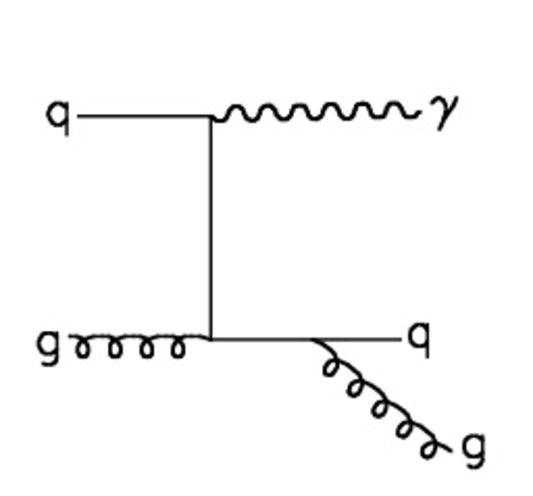
\includegraphics[scale=0.35]{p1j_compton.pdf}
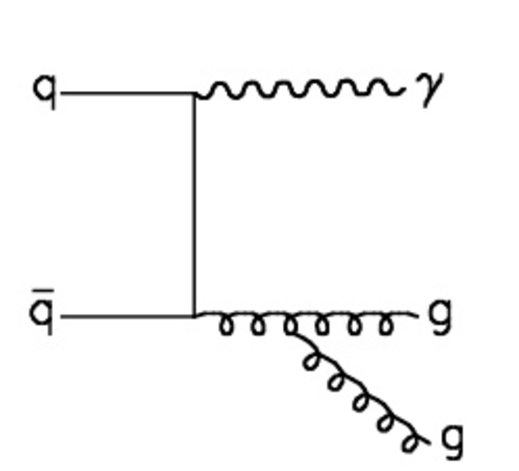
\includegraphics[scale=0.35]{p1j_annihilation.pdf}
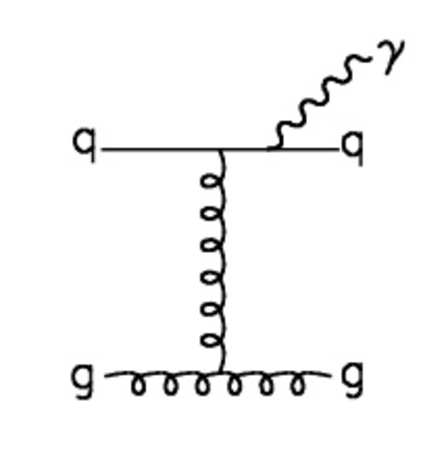
\includegraphics[scale=0.35]{p1j_brem.pdf}
%\end{minipage}
}
\qquad\qquad
\subfigure[]{\label{fig-gmsb-feyn}
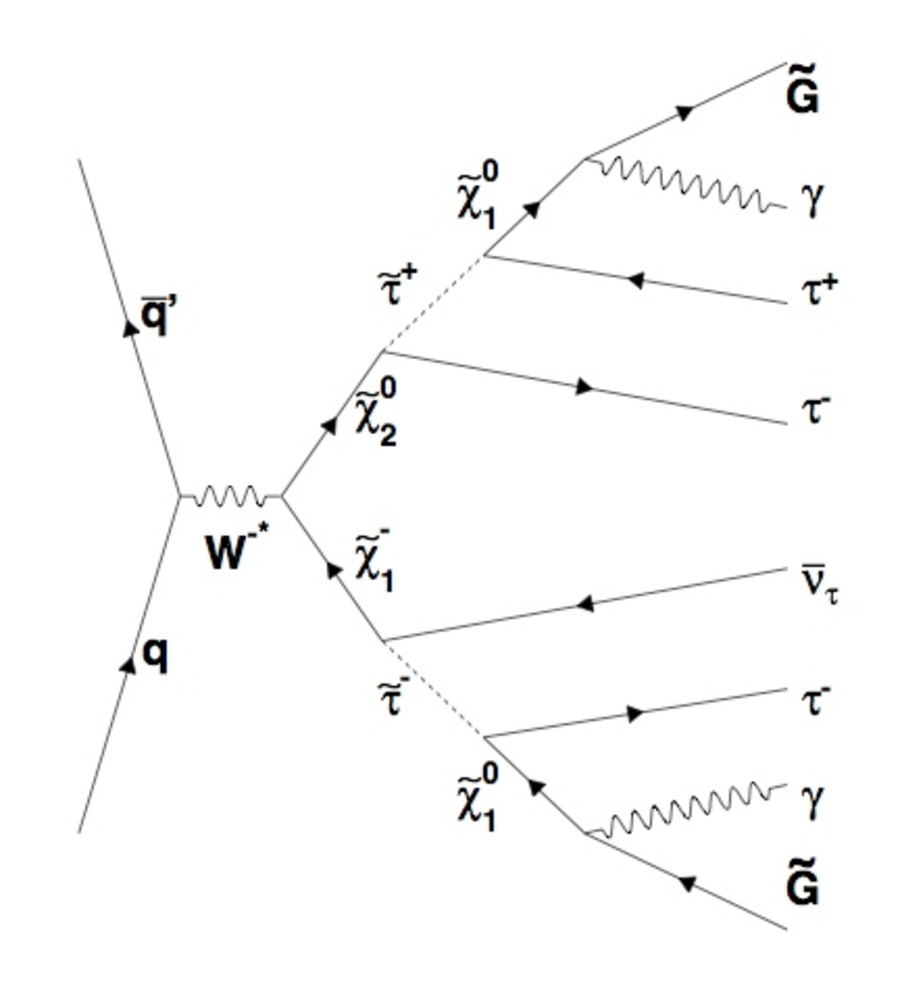
\includegraphics[scale=0.28]{gmsb_1.pdf}\quad
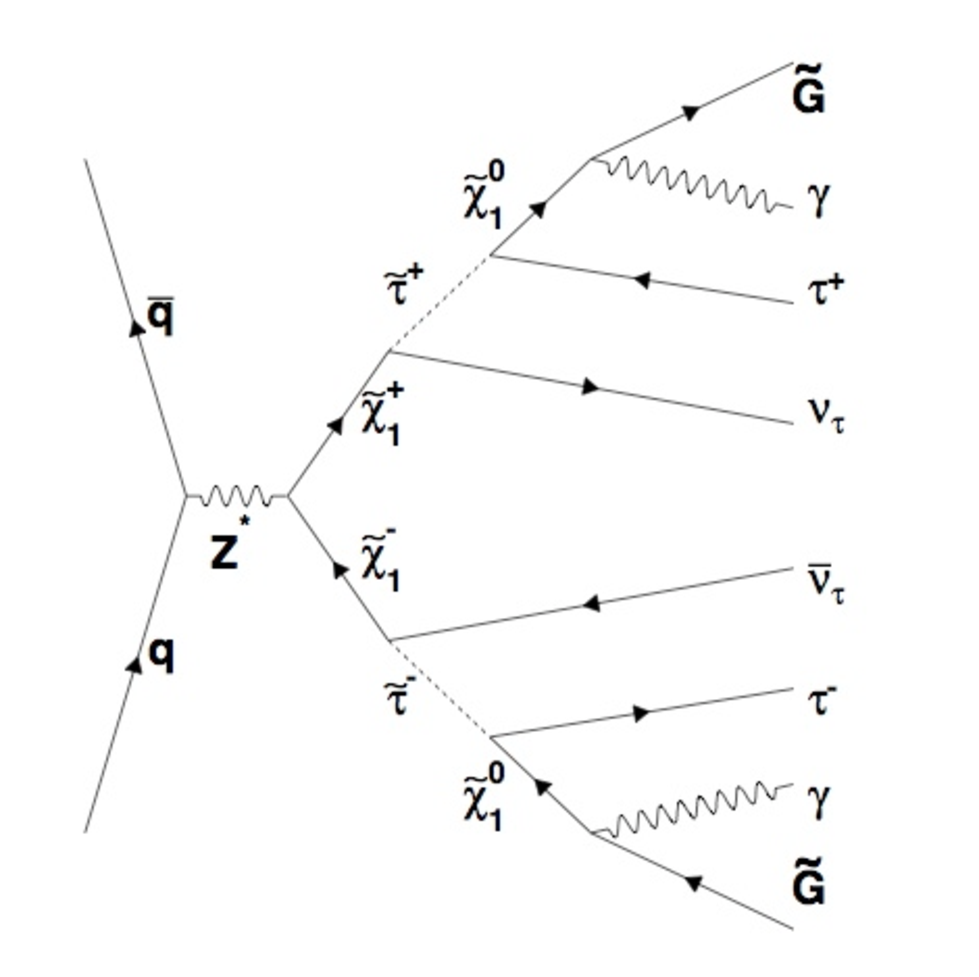
\includegraphics[scale=0.28]{gmsb_2.pdf}}
\caption{Feynman diagrams for tree-level (a) Standard Model and (b) GMSB processes that yield the $\gamma$~+~2 jets signature. The Standard Model processes have no intrinsic \met. A SUSY-like signal may be observed in \phojets events with large \met.}
\end{figure*}

We present two different methods of determining the backgrounds.  In the first method (Method A), we rely on a leading-order Monte Carlo generator (\textsc{pythia}) to predict the kinematic properties of jets in SM $\gamma$ + jets events.  In the second method (Method B), we employ a novel weighting technique that uses a combination of data and Monte Carlo to model higher-order QCD effects in kinematic distributions involving jets.

%%%%%%%%%%%%%%%%%%%%%%%%%%%%%%%%%%%%%%%%
% CDF Detector
%%%%%%%%%%%%%%%%%%%%%%%%%%%%%%%%%%%%%%%%
\section{CDF II Detector}
The Collider Detector at Fermilab (CDF) is  general purpose detector \cite{ref:CDFDetector}. It has a tracking system lying next to the beam pipe which is immersed in a superconducting solenoidal magnet providing a uniform 1.4~T magnetic field. The amount and the direction of a deflected charged particle is used to infer its momentum and charge. Outside of the solenoid are the calorimeters, which measure the energy of particles produced in the collision.

The tracking system comprised of a silicon pixel detector and open-cell drift chamber, central outer tracker (COT). The silicon detector and COT provides particle track information and the location of primary and secondary interaction points. The silicon system provides up to 8 measurements in the $r$ -- $\phi$ and $r$ -- $z$ views and covers the track reconstruction in the region $|\eta|<2$. The COT makes up to 96 measurements along the track of of each charge article in the region $|\eta|<1$. Sense wires are arranged in 8 alternating axial and $\pm3^{0}$ stereo super-layers. The resolution in \pt, $\sigma/p_{T}$, is $\approx 0.0015~p_{T}\cdot\mathrm{GeV^{-1}}\cdot c$ for track with only COT measurements, and $\approx 0.0007~p_{T}\cdot \mathrm{GeV}^{-1}\cdot c$ for tracks with both the silicon and the COT measurements. The calorimeter has two electromagnetic (EM) section and a hadronic section to stop and measure both  EM and hadronic particles. It has a projective tower geometry and is tower-segmented. The Central Preshower detector (CPR) lies after the drift chamber on the surface of the central calorimeter. CPR detector samples the early particle shower and improves photon identification and energy resolution. The Central Electromagnetic Shower Maximum detector (CES) is embedded in the central electromagnetic calorimeter and sample the lateral shower of the particle. It aids in separating neutral meson ($\pi^{0}$, $\eta$) decays from prompt photons.

CDF detector has a tower segmented calorimeter arranged in a projective geometry. Each calorimeter tower consists of an electromagnetic and a hadronic compartments \cite{ref:EMHADCals}. The central calorimeter covers the region $|\eta|<1.1$ and the `end plug' region extends from $1.1<|\eta|<3.6$. The central calorimeter is segmented in to 15$^{o}$ in $\phi$ and $\approx$0.1 in $\eta$ and has an \et resolution of $\sigma(E_{T})/E\approx 13.5\%\sqrt{E_{T}/\mathrm{GeV}} \oplus 2\%$ and the plug electromagnetic calorimeter has an energy resolution of $\sigma(\et)/\et = 16.0\%/\sqrt{\et} \oplus 2\%$. The central hadron calorimeter and plug hadron calorimeter energy resolution is $50\%\sqrt{E} \oplus 3\%$ and $80\%\sqrt{E} \oplus 5\%$ respectively.

CDF uses a cylindrical coordinate system with the $z$-axis along the axis of the colling beams. The variable $\theta$ is the polar angle relative to the incoming proton beam, and the variable $\phi$ is the azimuthal angle about the beam axis. The pseudorapidity of a particle trajectory is defined as $\eta=-\mathrm{ln(tan(}\theta/2))$. It is also useful to define detector pseudorapidity $\eta_{\mathrm{det}}$, denoting a particle's pseudorapidity in a coordinate system in which the origin lies at the center of the CDF detector rather than the at the event vertex. The transverse momentum \pt is the component of the momentum projected on a plane perpendicular to the beam axis.

%\section*{Object Identification}
%We require an energetic and isolated photon with $|\eta_{det}|<1.1$ and $p_{T}>$30~GeV identified using according to CDF standard criteria \cite{ref:PhotonIDAndCESCPR}. The isolation criteria roughly require less than 2~GeV of extra energy within a cone of $\Delta R = \sqrt{\Delta \eta^{2}+\Delta \phi^{2}}=0.4$ in $\eta$--$\phi$ space around the photon.

\section{Data Sample and Event Selection}
We select a sample of $\gamma$ candidates by identifying isolated electromagnetic clusters with \et~$>$~30~GeV in the central region of the central calorimeter ($|\eta^{detector}|<1.1$). In addition, we require the EM cluster to pass standard photon selection requirements~\cite{ref:PhotonIDAndCESCPR}. To reduce the background from charged leptons, we require an absence of tracks pointing in the direction of the EM cluster. The background from cosmic rays is reduced with a requirement on calorimeter EM timing~\cite{ref:EMtiming}, and we remove events that originate from the beam halo using a set of topological selection requirements~\cite{cdfnote:8409}. Events with photomultiplier tube spikes --- an instrumentation effect that can resemble a $\gamma$ --- are also removed. In the remaining event sample, we identify one or more jets with \mbox{\et$>15$~GeV} and $|\eta^{detector}|<3.0$. Jet energies are corrected for detector response, energy loss, multiple $p\bar{p}$ interactions and the underlying event \cite{pap:JetCorrections}. Furthermore, an azimuthal separation of $\Delta\phi>0.4$ radians between the direction of \met and any jet above \et$>15$~GeV is used to improve the energy measurement of jets.

After applying the event selection requirements described above, we select two data samples based on the number of jets with \et$>15$~GeV: \phoonejet events and \photwojet events. Within these two samples, subsamples with \mbox{\met$>20$~GeV} are identified. By selecting events with large \met, the dominant SM $\gamma$ and jet backgrounds are reduced, hence increasing our sensitivity to new physics. Various kinematic distributions in each of the four data samples are compared to the background expectation. %A typical $\gamma$ + jet event in the CDF detector is depicted in Fig.~\ref{fig-p1j-edited}.

\section{Modeling Backgrounds}\label{sec:modeling}
In this analysis we model backgrounds from two main sources:  SM processes and non-collision processes.  The SM processes include (1) prompt $\gamma$ production, (2) prompt diphoton production, (3) electroweak production of charged leptons that fake a prompt photon, and (4) QCD production of hadronic jets that fake a prompt photon.  The non-collision processes include energetic particles from cosmic rays and the beam halo that mimic the signal of a prompt photon from a $p\bar{p}$ collision. The \textsc{pythia} Monte Carlo generator (Tune~A) \cite{ref:pythia} is used to model SM prompt $\gamma$ production, prompt diphoton production, and the electroweak charged lepton backgrounds.  All other backgrounds are modeled using data.  For each of these SM backgrounds and the non-collision background, we construct a background template for each of the kinematic distributions under investigation.  The sum of these background templates is then compared to data.

SM diphotons are a significant source of fake \met background, as the probability to lose one of the photons in an uninstrumented region of the detector is twice as large as in a photon + jet event. The electroweak background is mainly from $W$, $Z$, $WW$, $WZ$, and $ZZ$ production, in which a final state lepton radiates a photon and we identify it as the prompt photon.

The background from QCD multijet production, in which a jet fakes a photon, is modeled using a sample that consists of jets that pass looser photon selection requirements (``sideband'' events). These jets are from neutral mesons like  $\pi^{0}$ and $\eta$ which decay almost exclusively to several photons. This energetic photons cannot be resolved well and are reconstructed as a single isolated photon.

Although a large portion of non-collision backgrounds from cosmic rays and the beam halo is removed by the \phojets selection requirements, some events remain, and these backgrounds are significant in the large \met subsamples. A pure cosmic ray event sample is attained using calorimeter EM timing information and is used to construct the background template. A set of topological cuts is used to select beam halo events.

We employ two different methods to construct templates from these background sources.  In both methods, the SM diphoton and SM charged lepton background templates are normalized to the expected number of events in the \phojets data using their respective Monte Carlo production cross sections and the integrated luminosity of the data. The cosmic ray and beam halo templates are normalized to the expected number of background events in the \phojets data.  The two methods differ in their treatment of the SM $\gamma$ background and the QCD multijet background, as described below.

\vspace{2ex}

\textbf{Method A}:  We model the SM prompt $\gamma$ production using the \textsc{pythia} Monte Carlo generator and the QCD multijet background from sideband events.  In Method A, these two background templates are scaled so that the total number of SM $\gamma$ events ($N^\mathrm{SM\gamma}$) and the total number of QCD multijet events ($N^\mathrm{QCD}$) satisfy
\begin{equation}
N^\mathrm{QCD} = f \cdot (N^\mathrm{SM\gamma}+N^\mathrm{QCD}),\label{eq:scaling}
\end{equation}
where $f$ is the fake photon fraction, which is determined to be
\begin{equation}
f~=~\mbox{0.319 $\pm$ 0.001(stat) $\pm$ 0.0068(syst)}\label{eq:fakefraction}
\end{equation}
from a study of inclusive photon data with photon \mbox{\et$>$ 30 GeV} \cite{ref:PhotonIDAndCESCPR}. In addition, the overall normalization of the SM $\gamma$ and QCD templates is adjusted so that the total number of background events from all sources equals the number of observed events in the data:
\begin{equation}
 N^\mathrm{Data} = N^\mathrm{SM\gamma}+N^\mathrm{QCD}+\underbrace{N^\mathrm{Di-\gamma}}_{fixed}+\underbrace{N^\mathrm{EWK}}_{fixed}+\underbrace{N^\mathrm{Non-collision}}_{fixed}.
\label{eqa:MtdANorm}
\end{equation}
When used together, Eqs.~\ref{eq:scaling} and \ref{eqa:MtdANorm} uniquely determine $N^\mathrm{SM\gamma}$ and $N^\mathrm{QCD}$.  We note that since the total number of events in the templates is constrained to match the total number of events in the data, our kinematic distributions are not sensitive to anomalies in the overall number of \phojets events, but they are sensitive to anomalies in the shapes of the distributions and excesses in the tails.

Table~\ref{tab:bgsummary1} summarizes the Method A background estimates for the \phoonejet and \photwojet samples.  Table~\ref{tab:bgsummary3} summarizes the Method A background estimates for the  \phoonejet + \met~$>$~20~GeV and \photwojet + \met~$>$~20~GeV samples.


%Using Method A, the overall fraction of background events from SM $\gamma$ is xxx\%.  This method includes all of the

%%%%%%%%%%%%%%%%%%%% Background Summary for g+jets sample %%%%%%%%%%%%%
\begin{table}[h!]
\begin{center}
\begin{tabular} {|c|c|c|}
\hline
\bf{Background} & \bf{\boldmath$\gamma$ + $\geq$1 Jet Sample} & \bf{\boldmath$\gamma$ + $\geq$2 Jet Sample} \\
\hline
Prompt $\gamma$ & 3387044 $\pm$ 1840  $\pm$ 108938&  629569 $\pm$ 793 $\pm$
39721\\
\hline
QCD & 1472467 $\pm$ 1213 $\pm$  27108 & 273681 $\pm$ 523 $\pm$
6095 \\
\hline
Electroweak & 11765 $\pm$ 108  $\pm$ 952& 1833 $\pm$ 42 $\pm$
271 \\
\hline
Diphoton & 12136 $\pm$ 110 $\pm$ 641 & 1775 $\pm$ 42 $\pm$
196 \\
\hline
Non-Collision & 132 $\pm$ 11  $\pm$ 4 & 8 $\pm$  2 $\pm$ 1 \\
\hline
\hline
\hline
\bf{\phojets Data} & 4883544 $\pm$ 2209 & 906866 $\pm$ 952\\
\hline
\end{tabular}
\end{center}
\caption{Summary of background estimates for the \phoonejet and \photwojet data samples evaluated by Method A.  Where two uncertainties are quoted, the first is statistical and the second is systematic.}
\label{tab:bgsummary1}
\end{table}


%%%%%%%%%%%%%%%%%%%% Background Summary for g+jets+MET>20 sample %%%%%%%%%%%%%
\begin{table}[h!]
\begin{center}
\begin{tabular} {|c|c|c|}
\hline
\bf{Background} & \bf{\boldmath$\gamma$ + $\geq$1 Jet + \met$>$~20 GeV} & \bf{\boldmath$\gamma$ + $\geq$2 Jet + \met$>$~20 GeV} \\
 & \bf{Sample} & \bf{Sample} \\
\hline
Prompt $\gamma$ & 88878 $\pm$ 366 $\pm$ 3178 & 28502 $\pm$ 168 $\pm$ 1429 \\
\hline
QCD & 38527 $\pm$ 196 $\pm$ 1664 & 12385 $\pm$ 111 $\pm$
524 \\
\hline
Electroweak & 6271 $\pm$ 79 $\pm$ 613 & 843 $\pm$ 29 $\pm$
122 \\
\hline
Diphoton & 355 $\pm$ 19 $\pm$ 13 & 86 $\pm$ 9 $\pm$
8 \\
\hline
Non-Collision & 124 $\pm$ 12 $\pm$ 4 & 8 $\pm$ 3 $\pm$ 1 \\
\hline
\hline
\hline
\bf{\phojets Data} & 134155 $\pm$ 366 & 41824 $\pm$ 204\\
\hline
\end{tabular}
\end{center}
\caption{Summary of background estimates for the \phoonejet + \met$>$~20 GeV and \photwojet + \met$>$~20 GeV data samples evaluated by Method A.  Where two uncertainties are quoted, the first is statistical and the second is systematic.}
\label{tab:bgsummary3}
\end{table}

In Method A, the background contributions from SM $\gamma$ events and QCD multijet events are expected to reproduce many of the kinematic distributions quite well; for example, photon \et and various invariant masses.  Nonetheless, the \textsc{pythia} Monte Carlo event generator used to generate the MC data samples includes only leading-order Feynman diagrams, and this limitation may be apparent in distributions like $H_T$ that rely on the accurate modeling of subleading jets.


%Hence, subleading jets are from parton showering, the underlying event, or from additional $p\bar{p}$ events that are overlayed on the primary hard scattering process.  The limitations of the leading-order MC generator may be apparent in distributions that rely on the correct modeling of jets.

%Hence the additional jets in MC data is derived from gluon radiation (parton showering). Also the jets created by radiation are often softer than the ones created by a hard scattering process. And this is not sufficient to describe data which has all next-to-leading order contributions and a complex mixture of different quark and gluon jets. This deficiency in MC data is clearly demonstrated by the discrepancy observed in the jet multiplicity distribution~\ref{fig:pjSetTwo:NJet} (xxx ref is wrong!!). This also affects the other distributions that depends on correct modeling of jets.

\vspace{2ex}

\textbf{Method B}:  In an attempt to overcome the limitations of using a leading-order Monte Carlo generator to model jet properties in $\gamma$ + jets events, we implement a novel method in which the QCD multijet events from the sideband data are used as a substitute for the \textsc{pythia} SM $\gamma$ events.  Although the QCD multijet events originate from a different physical process than prompt $\gamma$ + jets events, we hypothesize that these events, which come from actual data, describe the properties of jets in $\gamma$ + jets events better than leading-order Monte Carlo.  This should be readily apparent in distributions such as $H_T$ and the number of jets in the event.

%In order to overcome the limitations of using a leading-order Monte Carlo generator to model jet properties in $\gamma$ + jets events

%Hence, all subleading jets are from parton showering, the underlying event, or from additional $p\bar{p}$ events that are overlaid on the primary hard scattering process.

Since the sideband data presumably do not contain actual prompt photons, and are only QCD background, we do not expect the reconstructed ``QCD photons'' in those events to have the same \et distribution as the actual prompt photons from  \textsc{pythia}.  We therefore weight the events in the QCD background template in such a way that the weighted QCD template matches the sum of the \textsc{pythia} SM $\gamma$ and QCD templates for the photon \et distribution.  For an event in bin $i$ of the photon \et distribution, the associated weight is
\begin{equation}
w_i = \frac{N_i^{SM \gamma} + N_i^{QCD}}{N_i^{QCD}}\label{eq:weight}
\end{equation}
where $N_i^{SM \gamma}$ and $N_i^{QCD}$ are the contents of each bin $i$ of the background templates determined using Method~A.  Using Eq.~\ref{eq:weight}, a unique weight can be assigned to every event in the QCD background sample based on the bin $i$ of the QCD photon \et.

By defining a weight in this manner for every QCD background event, the QCD background template can be weighted for every kinematic distribution.  In all of the kinematic distributions, the weighted QCD template replaces the standard QCD template and the SM $\gamma$ template.  In the case of photon \et, by definition, the weighted QCD background template will be identical to the sum of the SM $\gamma$ and QCD templates.

This weighting procedure is referred to as Method B.  The weighted QCD template is normalized so that the total number of events, $N^\mathrm{Weighted-QCD}$, satisfies:

\begin{equation}
 N^\mathrm{Data} = N^\mathrm{Weighted-QCD}+\underbrace{N^\mathrm{Di-\gamma}}_{fixed}+\underbrace{N^\mathrm{EWK}}_{fixed}+\underbrace{N^\mathrm{Non-collision}}_{fixed}.
\label{eqa:MtdBnorm}
\end{equation}
As in Method A, we force the total number of background events to be equal to the total number of data events in each data sample studied.  We have calculated an additional systematic uncertainty for weighting procedure, and it is included in the plots of Method B distributions.

Table~\ref{tab:bgsummary2} summarizes the Method B background estimates for the \phoonejet and \photwojet samples.  Table~\ref{tab:bgsummary4} summarizes the Method B background estimates for the  \phoonejet + \met~$>$~20~GeV and \photwojet + \met~$>$~20~GeV samples.


%Table~\ref{tab:bgsummary2} summarizes the Method B background estimates for the \phoonejet and \photwojet data samples. As expected, Method B describes observed data in jet multiplicity distribution well. Also the distributions that directly depends on jets are improved significantly. But as expected this method fails to describe some distributions like the invariant mass of the $\gamma$ and the leading jet (see Fig. \ref{fig:pjMtdBSetOne:Mass_pj1}). This is due to the fact that SM prompt $\gamma$ + jet is modeled using di-jet mass which has many differences in terms of processes, color flow and detector resolution.

%%%%%%%%%%%%%%%%%%%% Background Summary for g+jets sample in Method B%%%%%%%%%%%%%
\begin{table}[h!]
\begin{center}
\begin{tabular} {|c|c|c|}
\hline
\bf{Background} & \bf{\boldmath$\gamma$ + $\geq$1 Jet Sample} & \bf{\boldmath$\gamma$ + $\geq$2 Jet Sample} \\
\hline
QCD (weighted) & 4859511 $\pm$ 2204 $\pm$ 149665 & 903250 $\pm$ 950 $\pm$ 44525 \\
\hline
Electroweak & 11765 $\pm$ 108  $\pm$ 952& 1833 $\pm$ 42 $\pm$
271 \\
\hline
Diphoton & 12136 $\pm$ 110 $\pm$ 641 & 1775 $\pm$ 42 $\pm$
196 \\
\hline
Non-Collision & 132 $\pm$ 11  $\pm$ 4 & 8 $\pm$  2 $\pm$ 1 \\
\hline
\hline
\hline
\bf{\phojets Data} & 4883544 $\pm$ 2209 & 906866 $\pm$ 952\\
\hline
\end{tabular}
\end{center}
\caption{Summary of background estimates for the \phoonejet and \photwojet data samples evaluated by Method B.  Where two uncertainties are quoted, the first is statistical and the second is systematic.}
\label{tab:bgsummary2}
\end{table}


%%%%%%%%%%%%%%%%%%%% Background Summary for g+jets+MET>20 sample %%%%%%%%%%%%%
\begin{table}[h!]
\begin{center}
\begin{tabular} {|c|c|c|}
\hline
\bf{Background} & \bf{\boldmath$\gamma$ + $\geq$1 Jet + \met$>$~20 GeV} & \bf{\boldmath$\gamma$ + $\geq$2 Jet + \met$>$~20 GeV} \\
 & \bf{Sample} & \bf{Sample} \\
\hline
QCD (weighted) & 127405 $\pm$ 357 $\pm$ 7040 & 40887 $\pm$ 202 $\pm$ 2103 \\
\hline
Electroweak & 6271 $\pm$ 79 $\pm$ 613 & 843 $\pm$ 29 $\pm$
122 \\
\hline
Diphoton & 355 $\pm$ 19 $\pm$ 13 & 86 $\pm$ 9 $\pm$
8 \\
\hline
Non-Collision & 124 $\pm$ 12 $\pm$ 4 & 8 $\pm$ 3 $\pm$ 1 \\
\hline
\hline
\hline
\bf{\phojets Data} & 134155 $\pm$ 366 & 41824 $\pm$ 204\\
\hline
\end{tabular}
\end{center}
\caption{Summary of background estimates for the \phoonejet + \met$>$~20 GeV and \photwojet + \met$>$~20 GeV data samples evaluated by Method B.  Where two uncertainties are quoted, the first is statistical and the second is systematic.}
\label{tab:bgsummary4}
\end{table}

%\section{Search for Resonance Decay}
%The invariant masses of final state decay products are searched for a resonance (bump) assuming a null hypothesis. For this a $\chi^{2}$ statistical test is performed as defined below.

%\begin{equation}
% \chi^{2} = \sum \frac{({\cal O}_{k} - E_{k})^{2}}{\sqrt{E_{k}}}
% \label{eqa:chi2Stat}
%\end{equation}

%\noindent where for a given bin $k$, ${\cal O}_{k}$ is the number of observed data events and $E_{k}$ is the expected number of events. We expect the number of data events per bin (${\cal O}_{k}$), to have an average value of $E_{k}$ and expected to fluctuate around $E_{k}$ with a standard deviation of order$\sqrt{E_{k}}$. If $\chi^{2}>>n$ where $n$ is the number of frequency bins, the  observed and the expected distributions differ significantly and we expect of a possible resonance production.

\section{Systematic Uncertainties}
The following systematic uncertainties are studied and a scale for each uncertainty is derived using different techniques. Any correlation across bins is ignored and all errors are added in quadrature to calculate the total systematic uncertainty. We have followed standard practices of quoting systematic uncertainties. All systematic uncertainties quoted are one standard deviation ($\pm1\sigma$) unless described otherwise.

The uncertainty in determining corrections to jet energies is taken into account as it changes the signal acceptance and the trigger efficiency, and hence the measured kinematic distributions. Uncertainties due to jet energy mismeasurements are obtained by varying the corrected jet energy by one standard deviation from the mean corrected value, \mbox{+$\sigma$} and \mbox{--$\sigma$}. A new set of events are selected from this shifted jet energy data. Each variation is compared to the nominal value, and the  maximum deviation from the nominal value is taken as the systematic uncertainty. The jet energy scale is by far the largest uncertainty in most of the measured distributions.

The uncertainty in the determination of the true photon fraction is described in literature ~\cite{ref:PhotonIDAndCESCPR} and is taken into account as follows. The normalization of the QCD template and the SM prompt photon template is changed by $\pm\sigma = \pm 0.068$ from the nominal value of the fake photon fraction, which is defined in Eq.~\ref{eqa:FakeFraction}. For each histogram bin, the maximum difference between the nominal distribution and the two varied ($\pm \sigma$) distributions is taken as the systematic uncertainty. This uncertainty makes a moderate contribution to the total systematic uncertainty. This uncertainty increases from about 10\% to about 40\% with increasing photon \et.

The uncertainty in the choice of photon sideband to represent the fake jets in the tight photon sample is estimated by varying the loose photon selection requirements to match the tight photon ID selection requirements. By doing so, one probes the sideband sample for the correlation to the tight photon sample. The selection requirements, Isolation Energy ($E_{T}^{\mathrm{Iso}}$), Had/Em ($E_{HAD}/E_{EM}$), Track \pt, and Track Isolation are common to both loose and tight photon selection requirements. Each of these loose photon selection requirements is set equal to the tight photon selection requirements one at a time, and four new sideband samples are selected. New samples are normalized back to the original (nominal) sideband sample and compared. The maximum deviation of each varied sample from the original sample is taken as the systematic uncertainty.

The acceptance and trigger efficiency depends on the Parton Distribution Functions (PDFs). The uncertainty in the PDFs used in MC event generation is derived following the recommendations of the CDF Joint Physics Group. Instead of generating many different sets of \MC event samples for each PDF set, {\sc CTEQ5L} events are reweighted to {\sc CTEQ6M} (next-to-leading order PDFs). The initial parton's information is approximated using generator-level information and 40~(+1) weights are generated for each of the 20 eigenvectors (higher and lower than nominal) and for a base distribution. Each kinematic distribution is remade according to the 40~(+1) generated weights. A maximum of 2 variations for each weight (representing an eigenvector) are added in quadrature to derive the total uncertainty. They are added in quadrature because these 20 eigenvectors are independent.

The dependence on the renormalization, factorization, and fragmentation scales (Q$^{2}$) are varied to estimate the higher-order contributions not considered by using leading-order MC signal sample. Two MC samples are generated by varying the nominal scale by 0.5 and 2.0. Each varied sample is normalized back to the nominal sample and the difference in shape from the nominal shape is taken as the systematic uncertainty. This systematic uncertainty is derived using only the generator-level objects. The leading photon is identified using generator-level information and hadron-level jets are used.

Uncertainty in the the amount of radiation from the incoming and outgoing partons is estimated by varying the corresponding \pythiaText parameters following the Joint Physics Group's recommendations. Five MC samples (more ISR, less ISR, more FSR, less FSR, and nominal) were needed. The MC samples for each variation are really a combination of many different MC sample with different $\hat{p}_{T}$, which are normalized by cross section to get the complete spectrum. Each of the four variations is normalized to the nominal distribution and the maximum variation of ISR and FSR is added in quadrature to derive the total systematic uncertainty.

The value of the strong coupling constant ($\alpha_s$) used in the generation of \MC event samples is not measured directly or absolutely. It is measured at the masses of the \pizero and $Z$-boson and then extrapolated to the other regions. An uncertainty for this is derived by comparing CTEQ5L PDF-based \MC events to MRST98 PDF-based \MC events, which use different values of \alphas when generating events.

The uncertainty in the measurement of the luminosity is approximately 6\% \cite{ref:CLCuncertainty}. Whenever a MC event sample is normalized by the luminosity, the uncertainty in the luminosity measurement needs to be taken into account. This is done by changing the luminosity by $\pm 6\%$ and recalculating the measurement. For every histogram bin, the maximum difference between these altered measurements and the nominal measurement is taken as the uncertainty due to the luminosity. The contribution of this uncertainty to the total uncertainty is relatively small.

The energy measured by the EM calorimeter carries a 1\% uncertainty. Hence, the photon candidate's energy is shifted by $\pm1\%$ and compared to the nominal distribution. The difference is taken as the systematic uncertainty due to the EM energy measurement.

As for the initial test methods, the statistical uncertainty in the cosmic photon template is taken as the systematic uncertainty for that bin. This uncertainty is very small and becomes somewhat significant in the high-\met region in the \met measurement.

Beam halo background is a very small background, and a constant 50\% uncertainty is assigned for its estimate.

In addition to above uncertainties, the uncertainty in the reweighting of the sideband events used in Method~B is derived by varying the fake photon fraction by its systematic uncertainty. This will change the fraction of SM $\gamma$ and QCD events chosen. The sideband events are reweighted using these alternate weights and the difference between these and the nominal distribution is taken as the uncertainty. This uncertainty increases from a few percent to about 10\% with increasing photon \et.

The JES is the largest systematic uncertainties in most of the measured distributions.

\section{Results}
\label{sec:PrelResults}
We present results in the \phojets data with and without the \met$>20$~GeV requirement.   In the \phoonejet and \photwojet event samples, we measure the \et of the photon, the \et of the leading jet, $H_{T}$ (scalar sum of all EM objects, jets and \met), \met, and invariant mass of photon and leading jet. In addition, in the \photwojet sample, we measure the invariant mass of the photon + two leading jets and the invariant mass of the two leading jets.

Figures \ref{fig:pjSetOne}--\ref{fig:pjSetFour} show Method A results without the \met requirement, and Figures \ref{fig:pjMetSetOne}--\ref{fig:pjMetSetFour} show Method A results with the \met requirement.  The data are represented by black circles, and the backgrounds are shown in different colors.  As described in Section~\ref{sec:modeling}, the SM backgrounds include prompt $\gamma$ production (labeled ``$\gamma$ MC''), QCD multijet production (labeled ``QCD''), prompt diphoton production (labeled ``Di-$\gamma$''), and electroweak production (labeled ``EWK'').  The non-collision backgrounds from cosmic rays and the beam halo are labeled ``Non-collision.''  The top plot uses a logarithmic scale. The shaded region indicates the total systematic uncertainty, which includes the statistical uncertainty on the total background prediction.

The uncertainty due to the jet energy scale is by far the largest systematic uncertainty. Other sources of uncertainty that are taken into account include the following:  parton density functions (PDFs), initial and final state radiation (ISR/FSR), dependence on the renormalization, factorization and normalization scales ($Q^{2}$), the strong coupling constant ($\alpha_{s}$), the fake photon fraction determination, integrated luminosity, EM energy measurements, the beam halo estimate, and the cosmic ray background estimate.

We have measured the photon \et spectrum from \mbox{30 GeV} to about \mbox{550 GeV}, and over this range the total systematic uncertainty increases from 15\% to 90\%. It is evident that the photon purity increases at higher \et.  We are limited by statistics at high \et. The invariant mass of the $\gamma$ + leading jet extends up to \mbox{1000 GeV/c$^{2}$}. Many background predictions become limited by statistics in the high mass region, and the systematic uncertainty increases from 15\% to 90\%. It is evident from these plots that the SM $\gamma$ and QCD multijet  backgrounds are dominant. However with the requirement of large \met in the event, these backgrounds are reduced and real \met from the electroweak processes ({\it e.g.} $W \to \ell \nu$) becomes significant. This \met requirement significantly improves the sensitivity to events in which a heavy particle is produced that we do not detect.

The backgrounds using Method A are well modeled and describe data reasonably well in most of the distributions. But a close inspection reveals discrepancies in certain distributions like lead jet \et, $H_{T}$, jet multiplicity, and \met, which are not within the systematic uncertainties.  These kinematic distributions are most directly affected by the limitations of the leading-order predictions using \textsc{pythia}.


% So we opted to further investigate and understand our background modeling in an attempt to understand the causes of such discrepancies.

%It is well known that MC programs have limitations in including next-to-leading order calculations.

%The \textsc{pythia} Monte Carlo event generator that we have used to generate the MC data samples includes only leading-order Feynman diagrams. Hence, all subleading jets are from parton showering, the underlying event, or from additional $p\bar{p}$ events that are overlaid on the primary hard scattering process. This directly affects the aforementioned kinematic variables. Furthermore, this causes the calorimeter \met resolution for MC data to differ from collision data. Hence, it is difficult to describe the low \met is region which is dominated by fake \met from jet energy mismeasurements using MC data.


Figures \ref{fig:pjMtdBSetOne}--\ref{fig:pjMtdBSetFour} show the Method~B results without the \met requirement. The Figures \ref{fig:pjmetMtdBSetOne}--\ref{fig:pjmetMtdBSetFour} show the Method~B results with the \met requirement.  In these figures, ``QCD (weighted)'' indicates the weighted QCD background template that replaces the $\gamma$ MC and QCD templates of Method A.  Using Method B, we are able describe some distributions much better compared to Method A. The photon \et distribution must agree with Method A by construction. The jet \et, $H_{T}$, jet multiplicity and \met distributions, however, show significant improvement and agree well with data. The \met distribution agrees well in the low \met region. Some distributions using Method B were not modeled well as expected. For example the invariant mass of the photon and leading jet shows a large discrepancy, which is attributed to the fact that the QCD background events are from different processes (or Feynman diagrams).

\section{Conclusions}
We have presented results of the search for beyond SM physics in \phoonejet and \photwojet events with and without a \met~$>$~20~GeV requirement. We have presented two different background prediction methods, Method A and Method B. Each method has proven to describe the \phojets data with certain limitations. We conclude the two methods together provide a greater understanding of data than either method alone. Thus far, we see good agreement with Standard Model predictions extending over several orders of magnitude. The search for new heavy particles in the high \met events has shown no significant deviation from data. We conclude that all of our measurements are in agreement with the Standard Model expectation.

%The search for a narrow resonance using the reconstructed masses of $\gamma$ and the leading jet, $\gamma$ and the leading two jets, and the two leading jets, has not shown a significant difference between distribution of data and the expected distribution. And hence no indication of heavy particle decay or new production mechanisms.


\section{Acknowledgements}
%For PRD change to:
%\begin{acknowledgments}
%check for the latest@
%http://www-cdf.fnal.gov/internal/people/links/CarolPicciolo/standardack.html
We thank the Fermilab staff and the technical staffs of the participating institutions for their vital contributions. This work was supported by the U.S. Department of Energy and National Science Foundation; the Italian Istituto Nazionale di Fisica Nucleare; the Ministry of Education, Culture, Sports, Science and Technology of Japan; the Natural Sciences and Engineering Research Council of Canada; the National Science Council of the Republic of China; the Swiss National Science Foundation; the A.P. Sloan Foundation; the Bundesministerium f\"ur Bildung und Forschung, Germany; the World Class University Program, the National Research Foundation of Korea; the Science and Technology Facilities Council and the Royal Society, UK; the Institut National de Physique Nucleaire et Physique des Particules/CNRS; the Russian Foundation for Basic Research; the Ministerio de Ciencia e Innovaci\'{o}n, and Programa Consolider-Ingenio 2010, Spain; the Slovak R\&D Agency; and the Academy of Finland.
%\end{acknowledgments}

\begin{thebibliography}{99}
\bibitem{ref:CDFDetector}
F. Abe \textit{et al}., Nucl. Instrum. Methods Phys. Res. A {\bf 271}, 387 (1988);
D. Amidei \textit{et al}., Nucl. Instum. Methods Phys. Res. A {\bf 350}, 73 (1994);
F. Abe et al., Phys. Rev. D {\bf 52}, 4784 (1995);
P. Azzi \textit{et al}., Nucl. Instrum. Methods Phys. Res. A {\bf
360}, 137 (1995);
The CDF II Detector Technical Design Report, Fermilab-Pub-96/390-E.

\bibitem{ref:models}
See for example S. Ambrosanio \textit{et al}., Phys. Rev. D \textbf{54}, 5395 (1996); or C.-H. Chen and J.F. Gunion, Phys. Rev. D \textbf{58}, 075005 (1998).

\bibitem{ref:TechnicolorModel}
  S. Weinberg, ``Implications of Dynamical Symmetry Breaking: An Addendum'' Phys. Rev. D {\bf 19}, 1277--1280 (1979);
  L. Susskind, ``Dynamics of Spontaneous Symmetry Breaking in the Weinberg-Salam Theory'' Phys. Rev. D {\bf 20}, 2619--2625 (1979).

\bibitem{ref:PhotonIDAndCESCPR} F. Abe \textit{et al}., ``Prompt photon cross section measurement in $\bar{p}p$ collisions at $\sqrt{s}$ = 1.8 TeV'', Phys. Rev. D {\bf 48}, 2998--3025 (1993);
 F. Abe \textit{et al}., ``Precision Measurement of the Prompt Photon Cross Section in $p\bar{p}$ Collisions at $\sqrt{s}$ = 1.8 TeV'', Phys. Rev. Lett. {\bf 73}, 2662 (1994);
 D. Acosta {\textit et al.} (CDF Collaboration), Phys. Rev. Lett. {\bf 95}, 092004 (2007);  The CDF Collaboration, ``Search for Anomalous Production of Events with a Photon, Jet, $b$-quark Jet, and Missing Transverse Energy '', Phys. Rev. D {\bf 80} (2009).

\bibitem{ref:EMtiming}
``The Timing System for the CDF Electromagnetic Calorimeters,'' Nucl. Instrum. Meth. {\bf A565}, 543--550, 2006.

\bibitem{cdfnote:8409} M. Goncharov \textit{et al}., ``Discrimination of Beam Halo and Cosmic Rays as a Source of Photon Candidates,'' CDF-Note 8409.

\bibitem{pap:JetCorrections} The CDF Collaboration, ``Determination of the Jet Energy Scale at the Collider Detector at Fermilab,'' Nucl. Instrum. Meth. \textbf{A566}, 375--412, 2006.

\bibitem{ref:pythia}
T. Sj\"{o}strand \textit{et al}., Comput. Phys. Commun. \textbf{135}, 238 (2001).


\bibitem{ref:CLCuncertainty} D. Acosta \textit{et al}., Nucl. Instrum. Methods, \textbf{A494}, 57 (2002).

\bibitem{ref:EMHADCals}  L. Balka \textit{et al}. Nucl. Instrum. Methods \textbf{267}, 272 (1988); S. Bertolucci \textit{et al}. Nucl. Instrum. Methods \textbf{267}, 301 (1988); S. Kuhlmann \textit{et al}., Nucl. Instrum. Methods \textbf{518}, 39, 2004.


%\bibitem{exp:TrnPlane} \et is the calorimeter energy as measured in the transverse plane.
\end{thebibliography}




\clearpage
%%%%%%%%%%%%%%%%%%%%%%%%%%%%%% METHOD A: G30 JETS
\begin{figure*}[h!]
\centering
\caption[Method A \phoonejet]{Kinematic distributions of \phoonejet events using Method A. See Section~\ref{sec:PrelResults} for a description of the elements in these distributions.}
\subfigure[]
{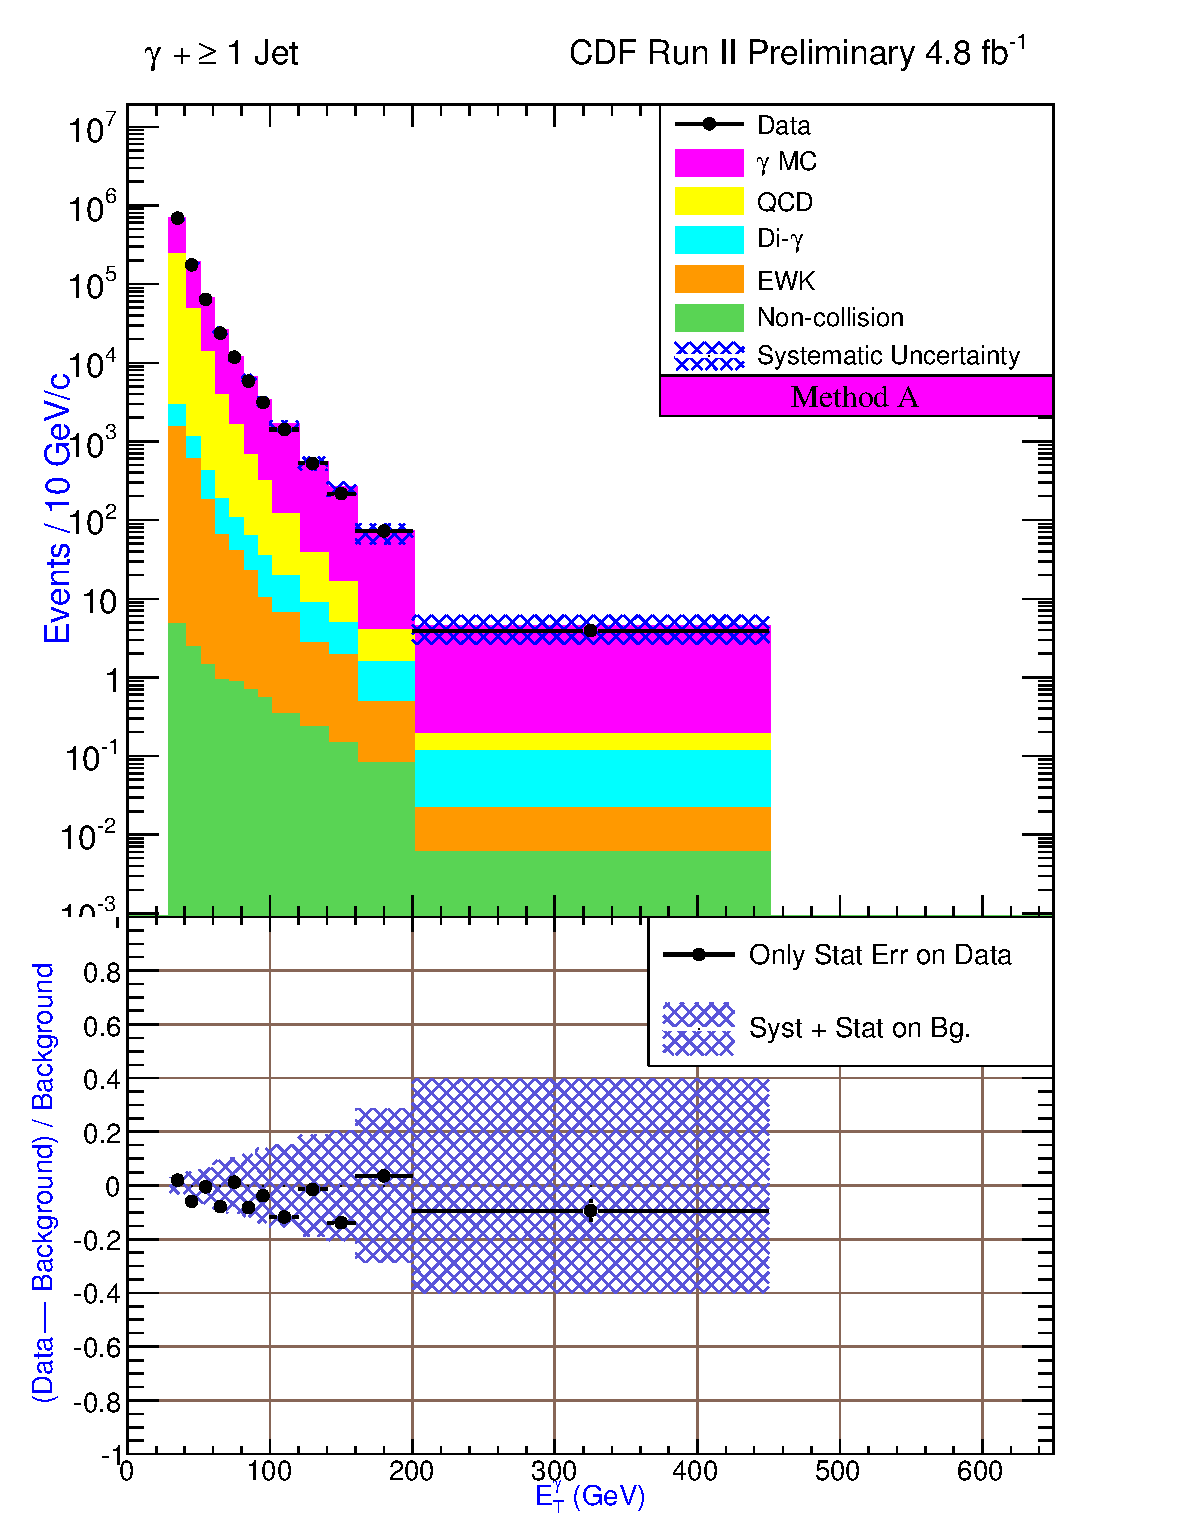
\includegraphics[keepaspectratio=true, scale=\figScale]{G30Jets_MtdA_plot1_Et_pho.pdf}}
\subfigure[]
{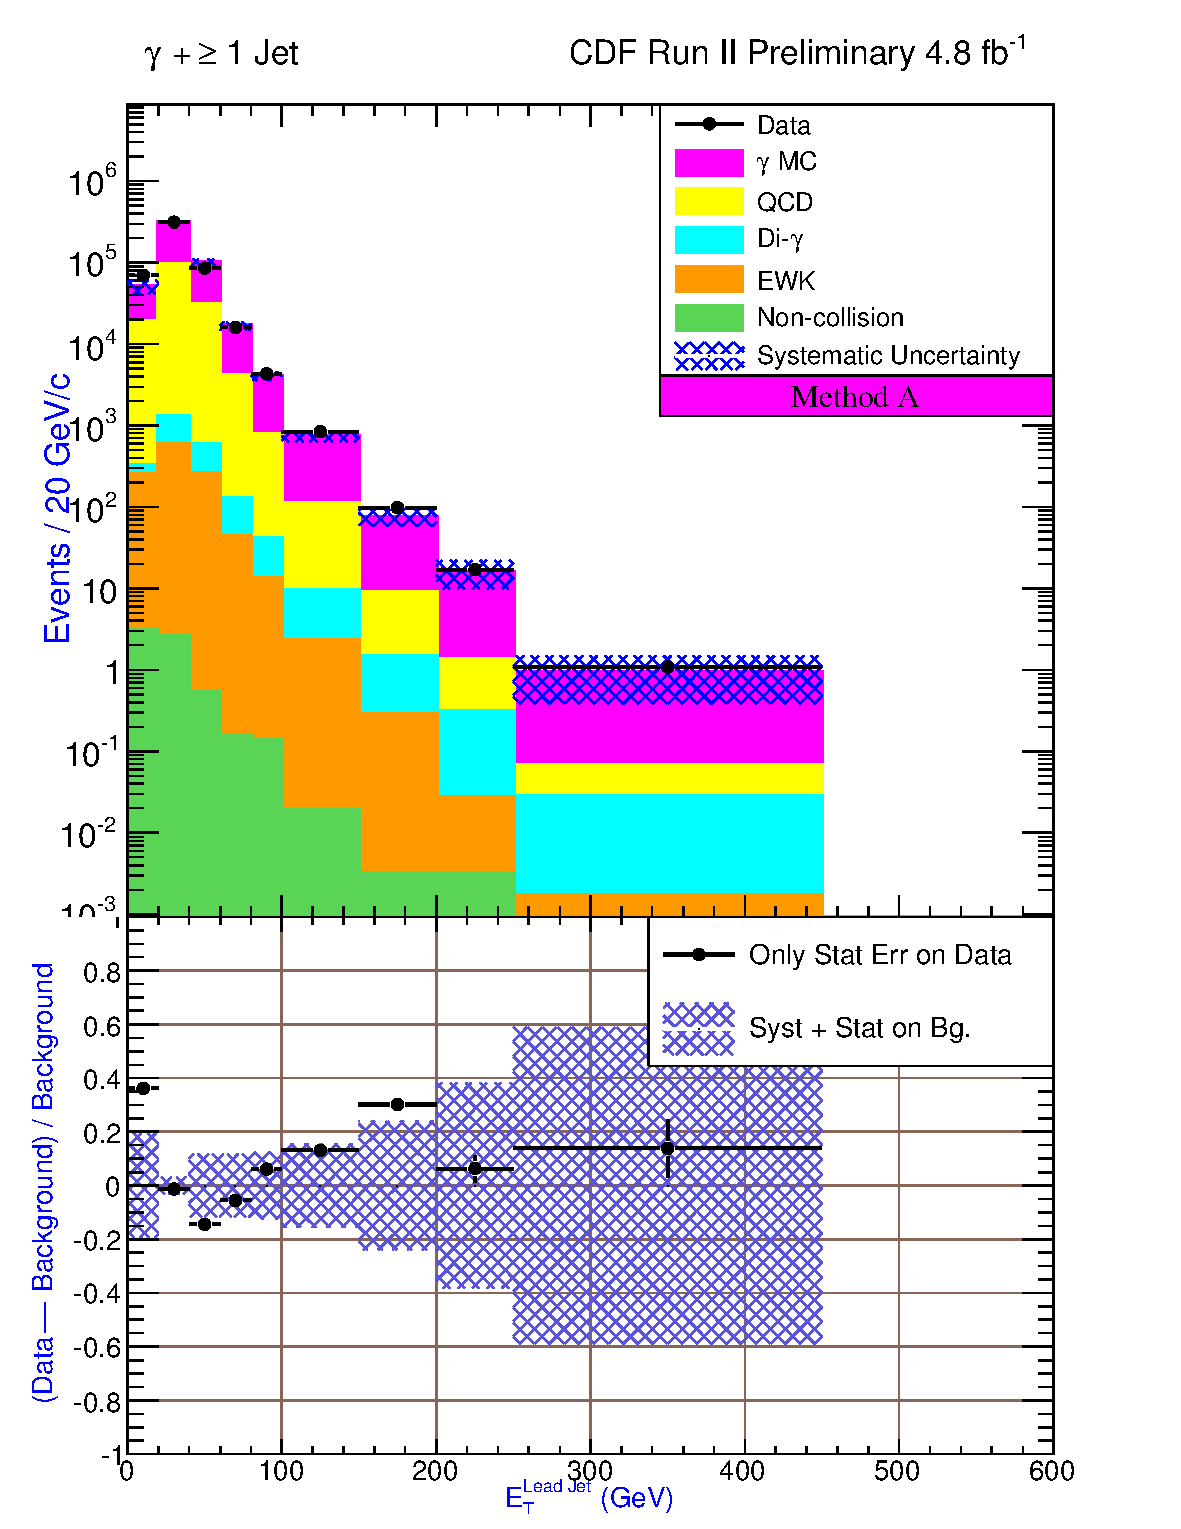
\includegraphics[keepaspectratio=true, scale=\figScale]{G30Jets_MtdA_plot1_Et_j1.pdf}
}

\subfigure[]
{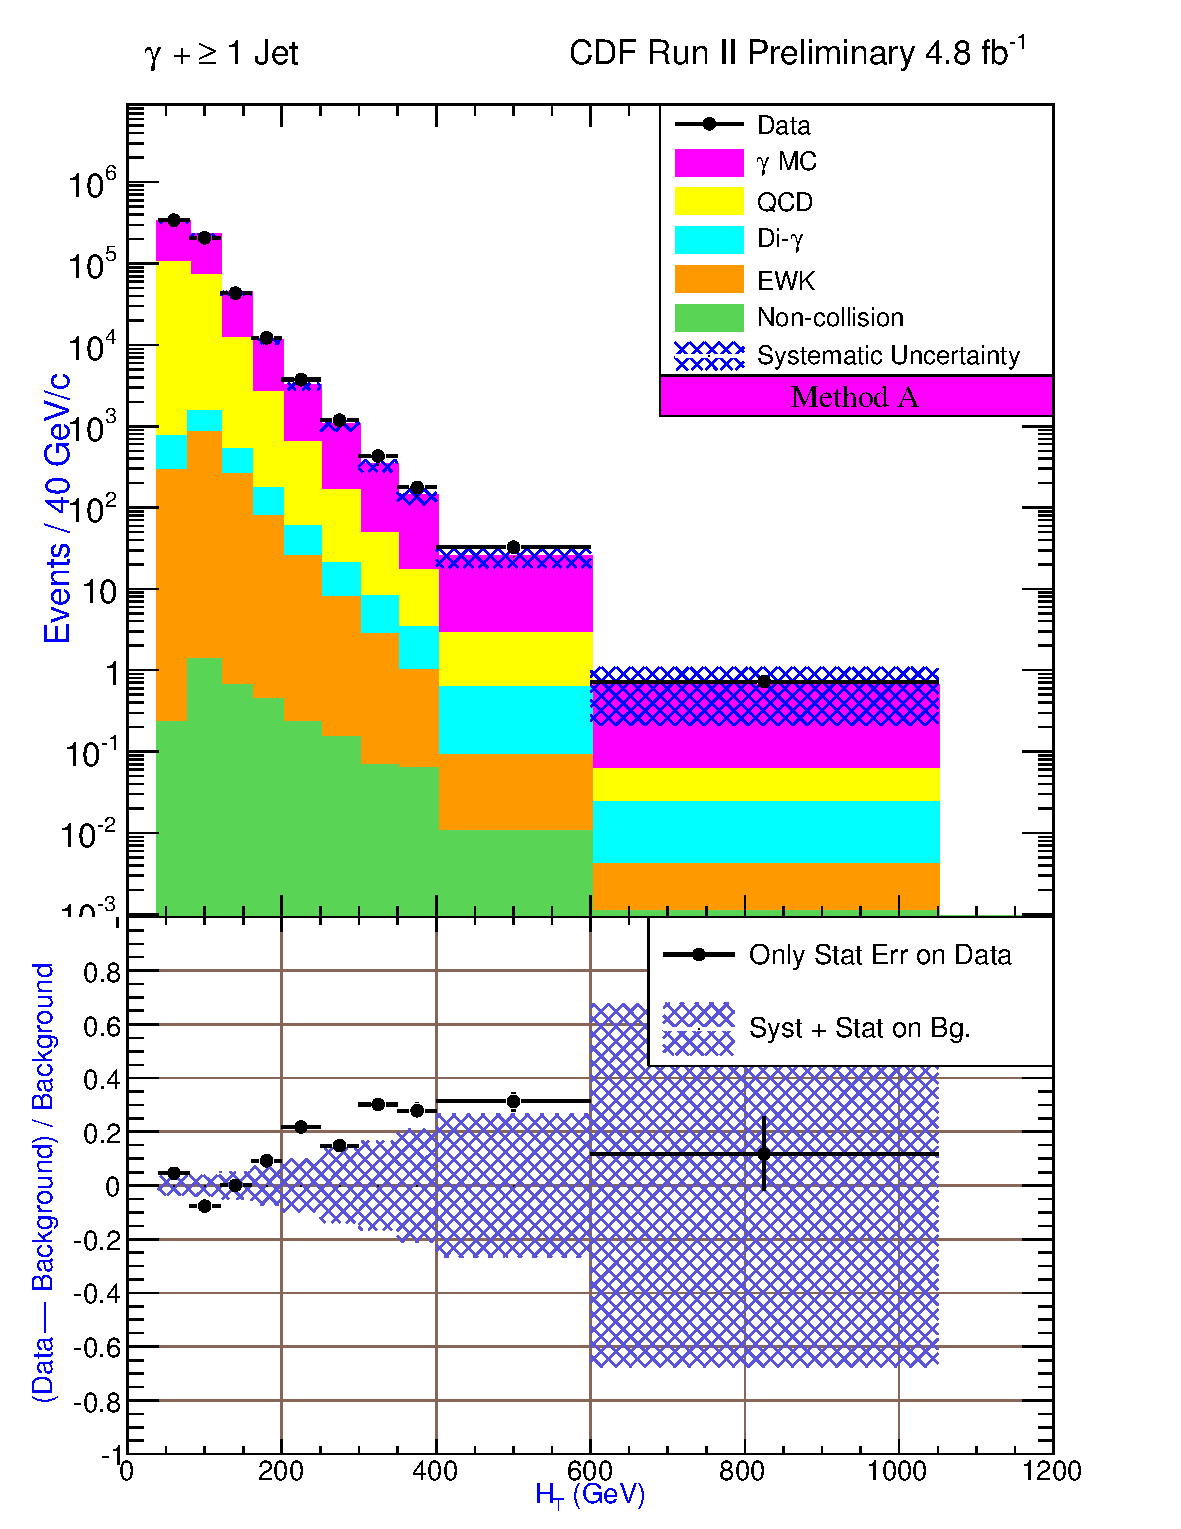
\includegraphics[keepaspectratio=true, scale=\figScale]{G30Jets_MtdA_plot1_Ht.pdf}}
\subfigure[]
{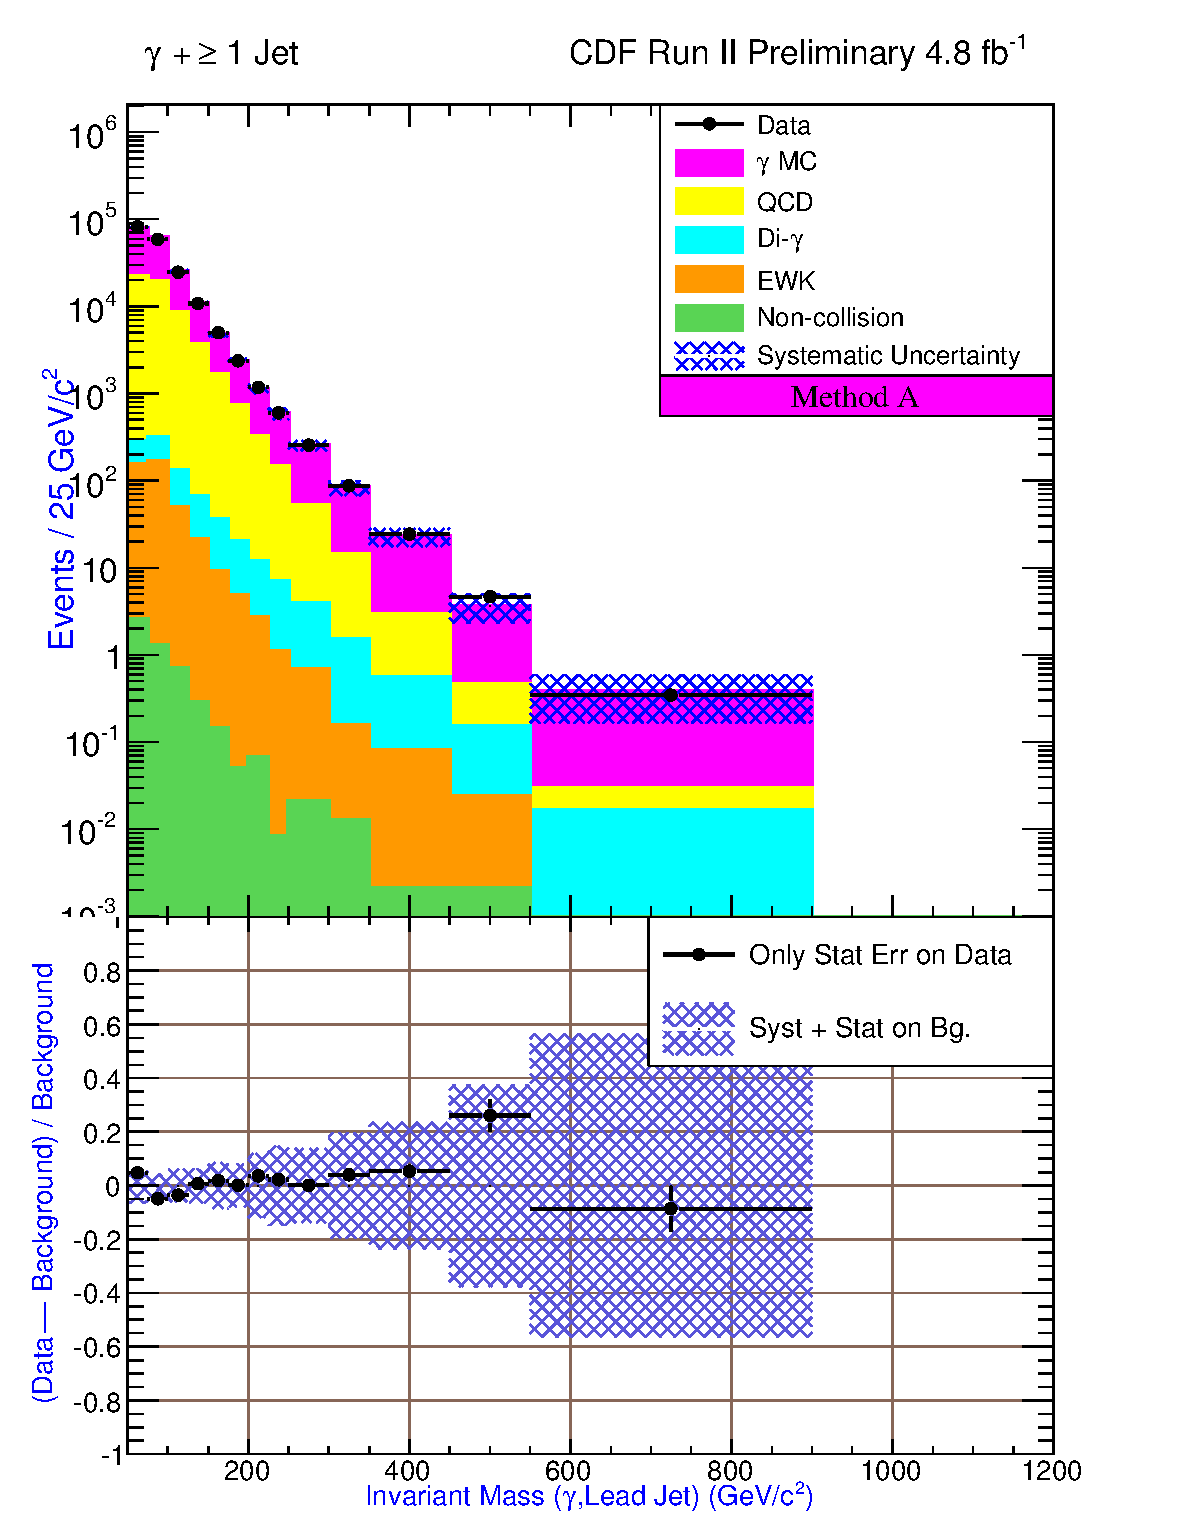
\includegraphics[keepaspectratio=true, scale=\figScale]{G30Jets_MtdA_plot1_InvMass_pj1.pdf}}
\label{fig:pjSetOne}
\end{figure*}
\clearpage

\begin{figure*}[h!]
\label{fig:pjSetTwo}
\centering
\caption[Method A \phoonejet]{Kinematic distributions of \phoonejet (top) and \photwojet (bottom) events using Method A. See Section~\ref{sec:PrelResults} for a description of the elements in these distributions.}
\subfigure[]
{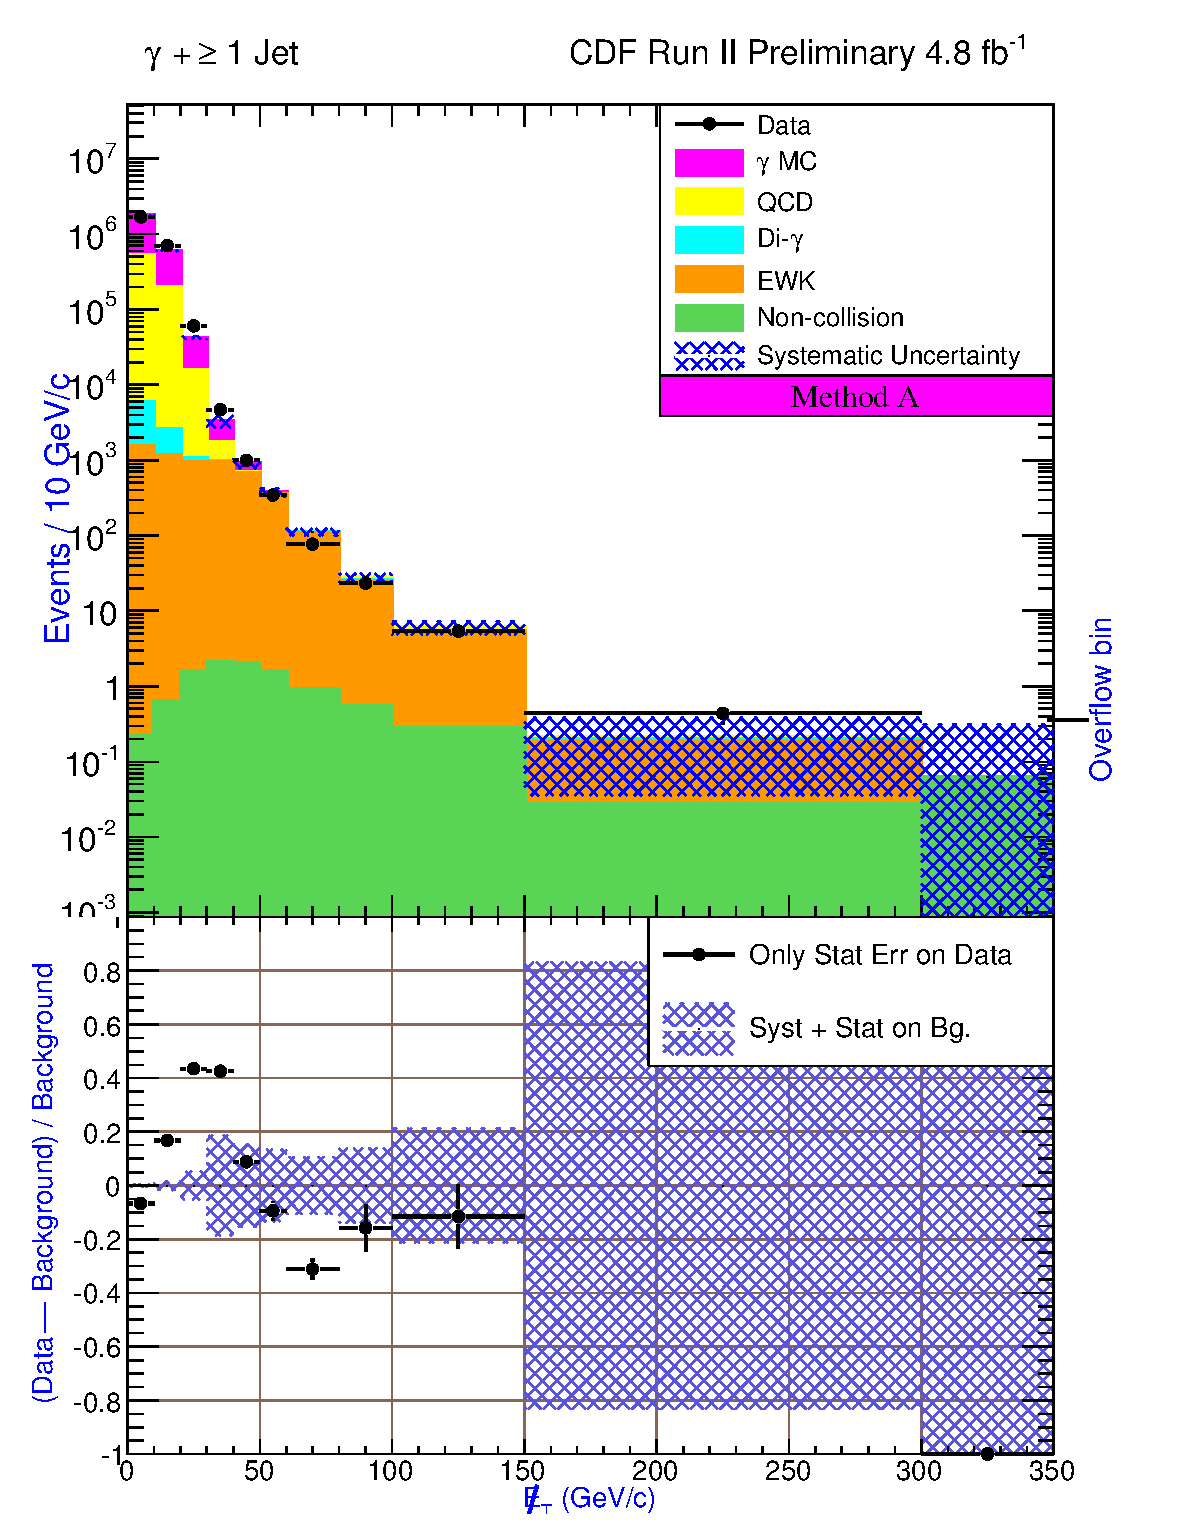
\includegraphics[keepaspectratio=true, scale=\figScale]{G30Jets_MtdA_plot1_Met.pdf}}
\subfigure[]
{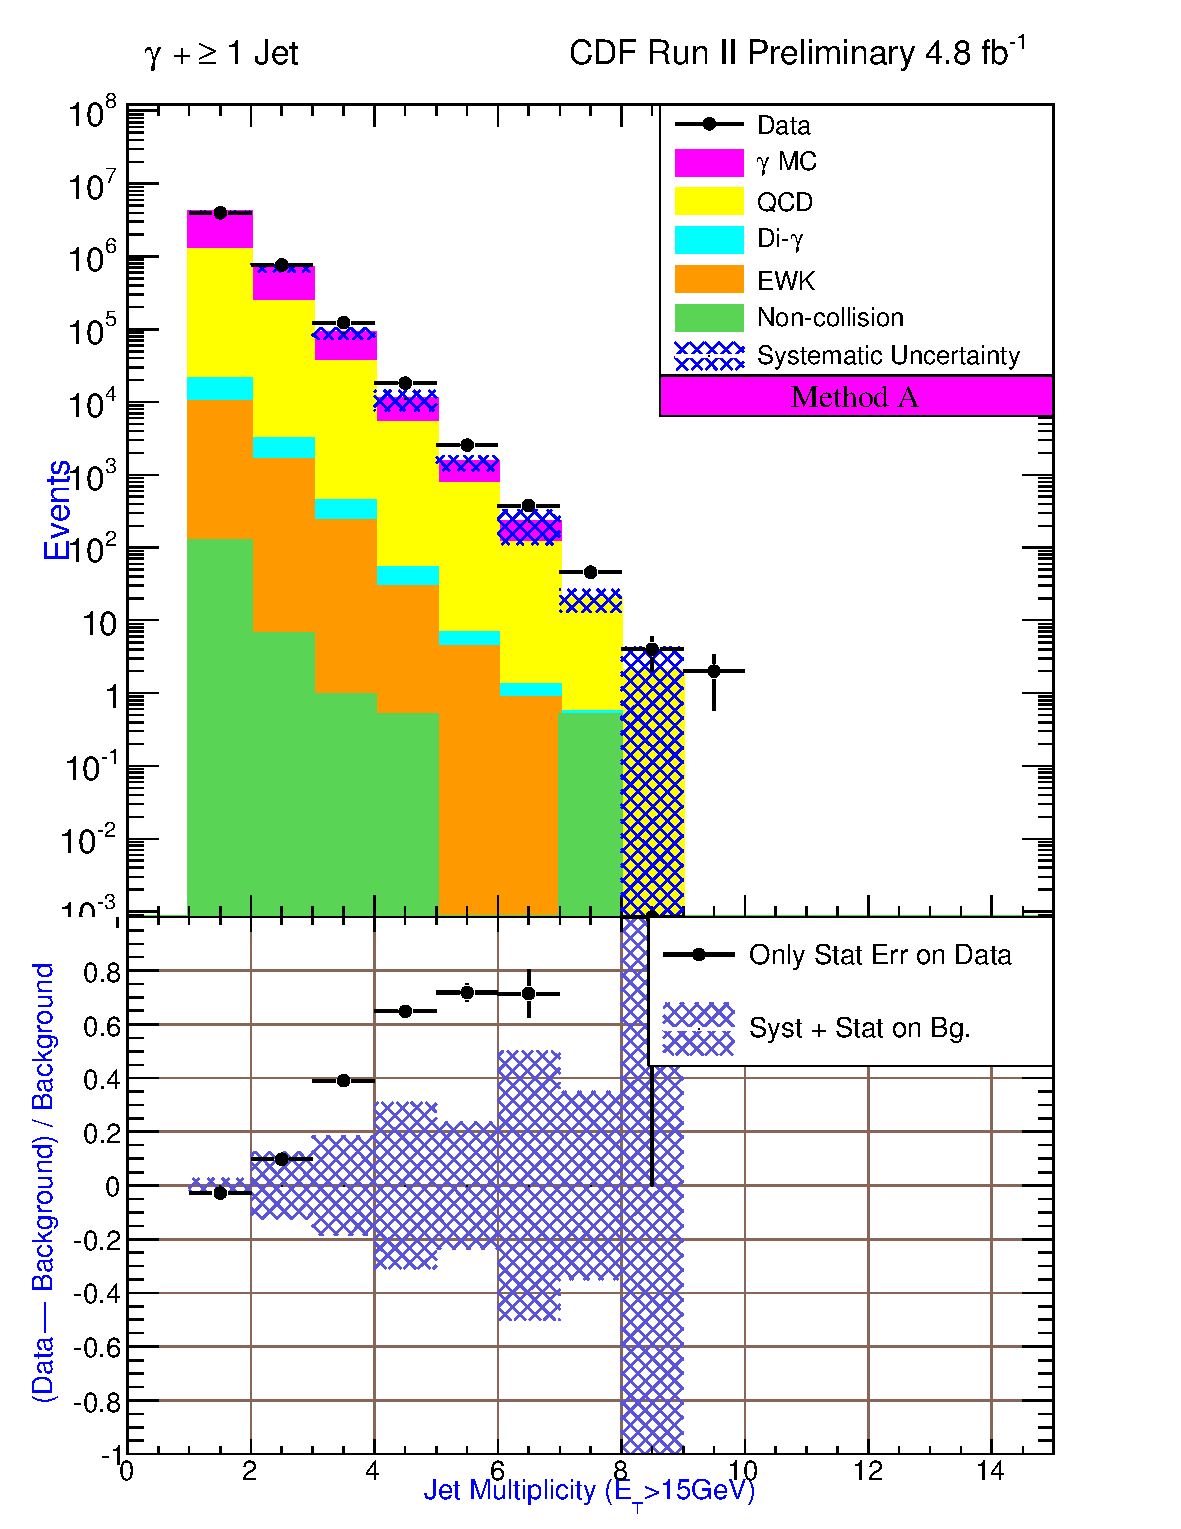
\includegraphics[keepaspectratio=true, scale=\figScale]{G30Jets_MtdA_plot1_NJet.pdf}\label{fig:pjSetTwo:NJet}}
\subfigure[]
{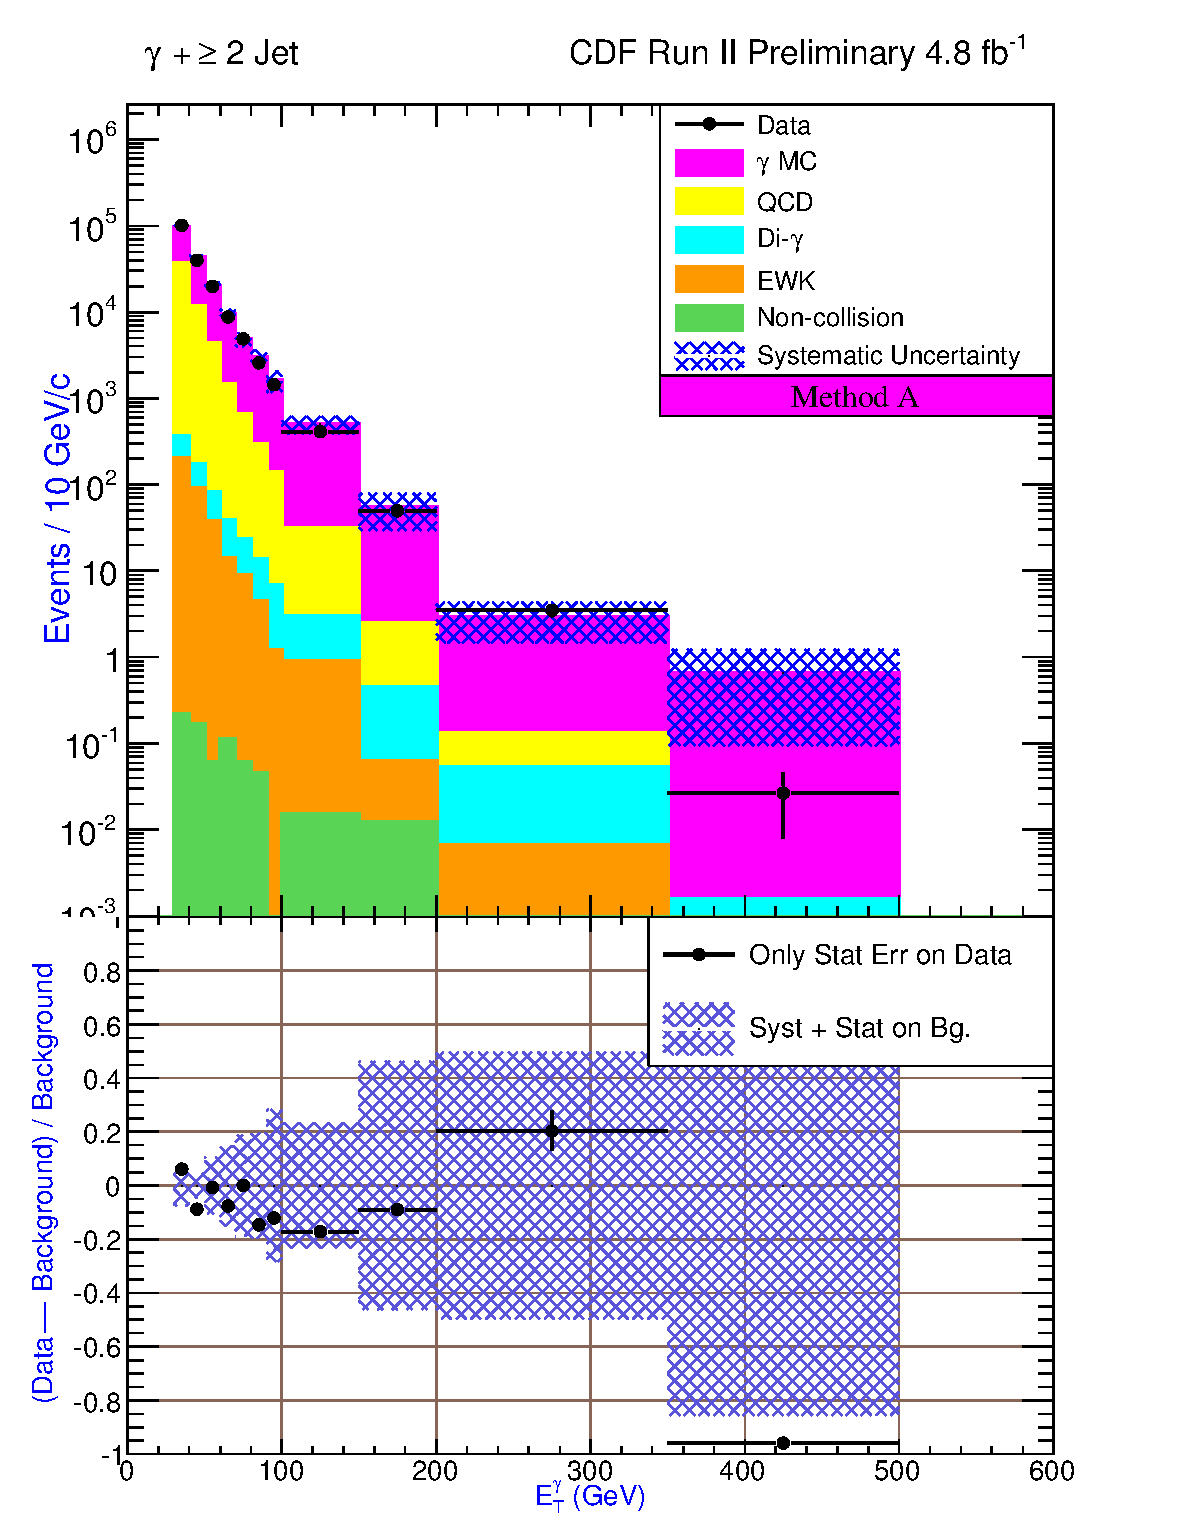
\includegraphics[keepaspectratio=true, scale=\figScale]{G30Jets_MtdA_plot2_Et_pho.pdf}}
\subfigure[]
{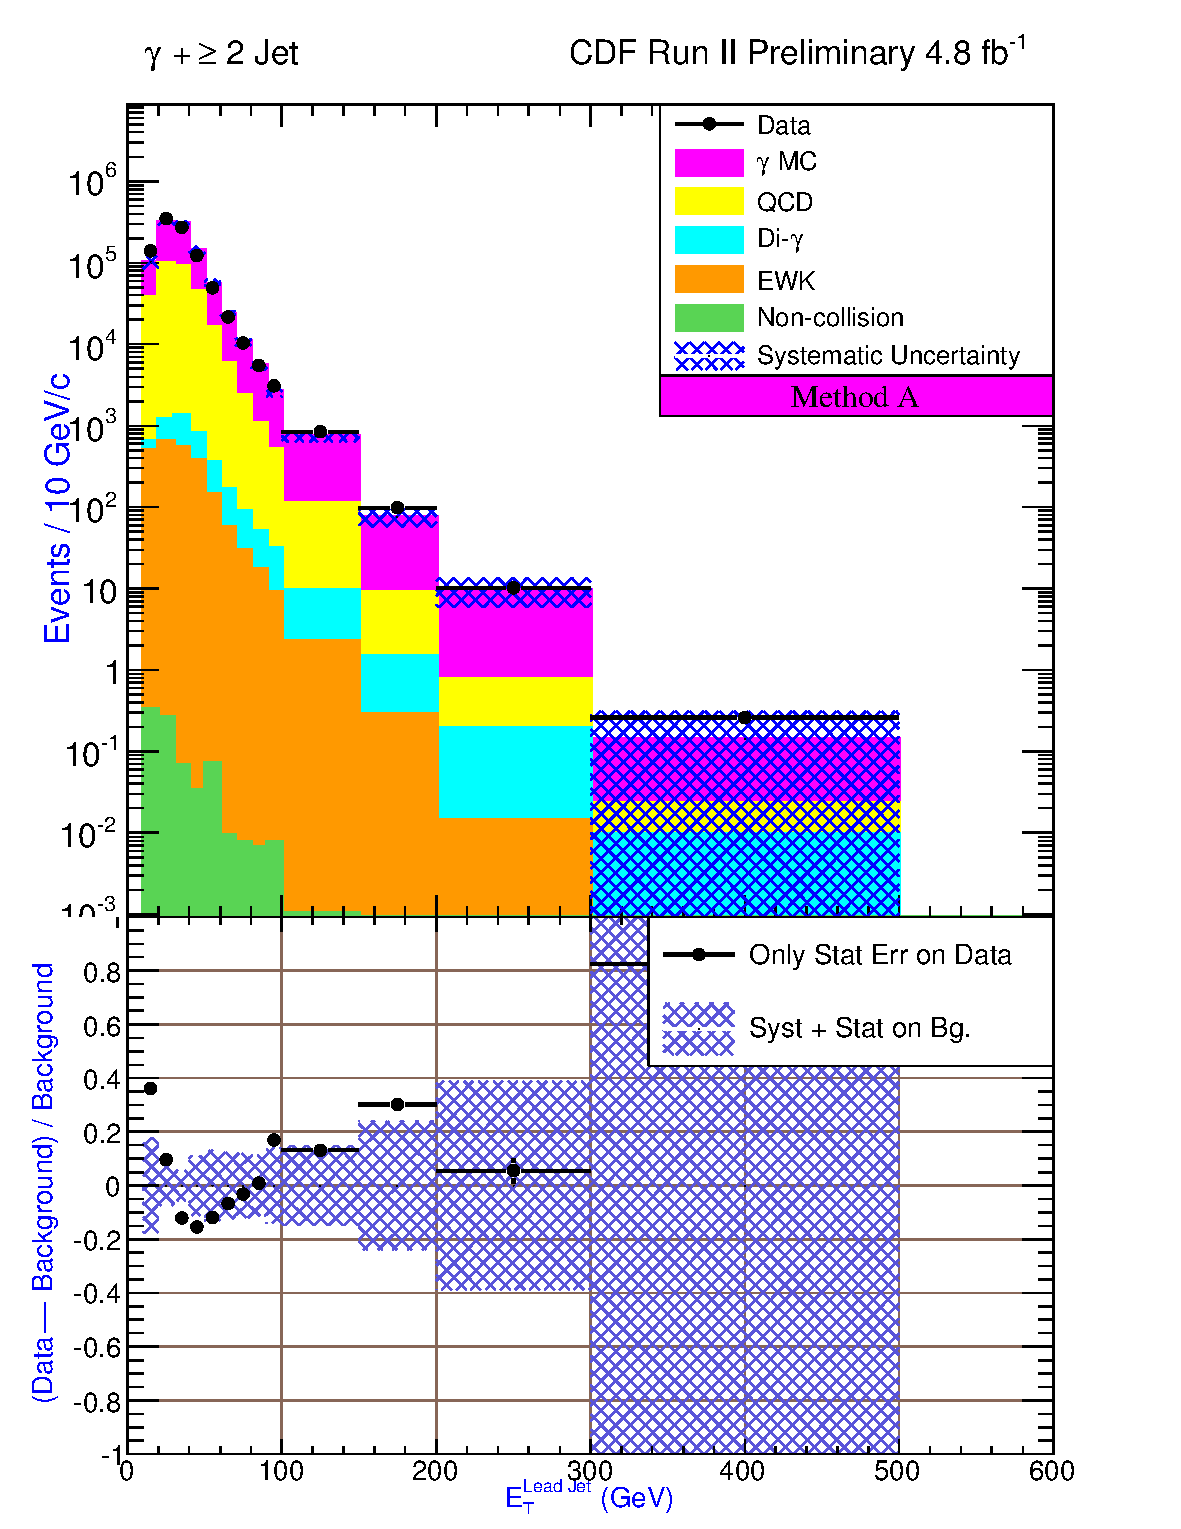
\includegraphics[keepaspectratio=true, scale=\figScale]{G30Jets_MtdA_plot2_Et_j1.pdf}}
\end{figure*}
\clearpage

\begin{figure*}[h!]
\centering
\caption[Method A \phoonejet]{Kinematic distributions of \photwojet events using Method A. See Section~\ref{sec:PrelResults} for a description of the elements in these distributions.}
\subfigure[]
{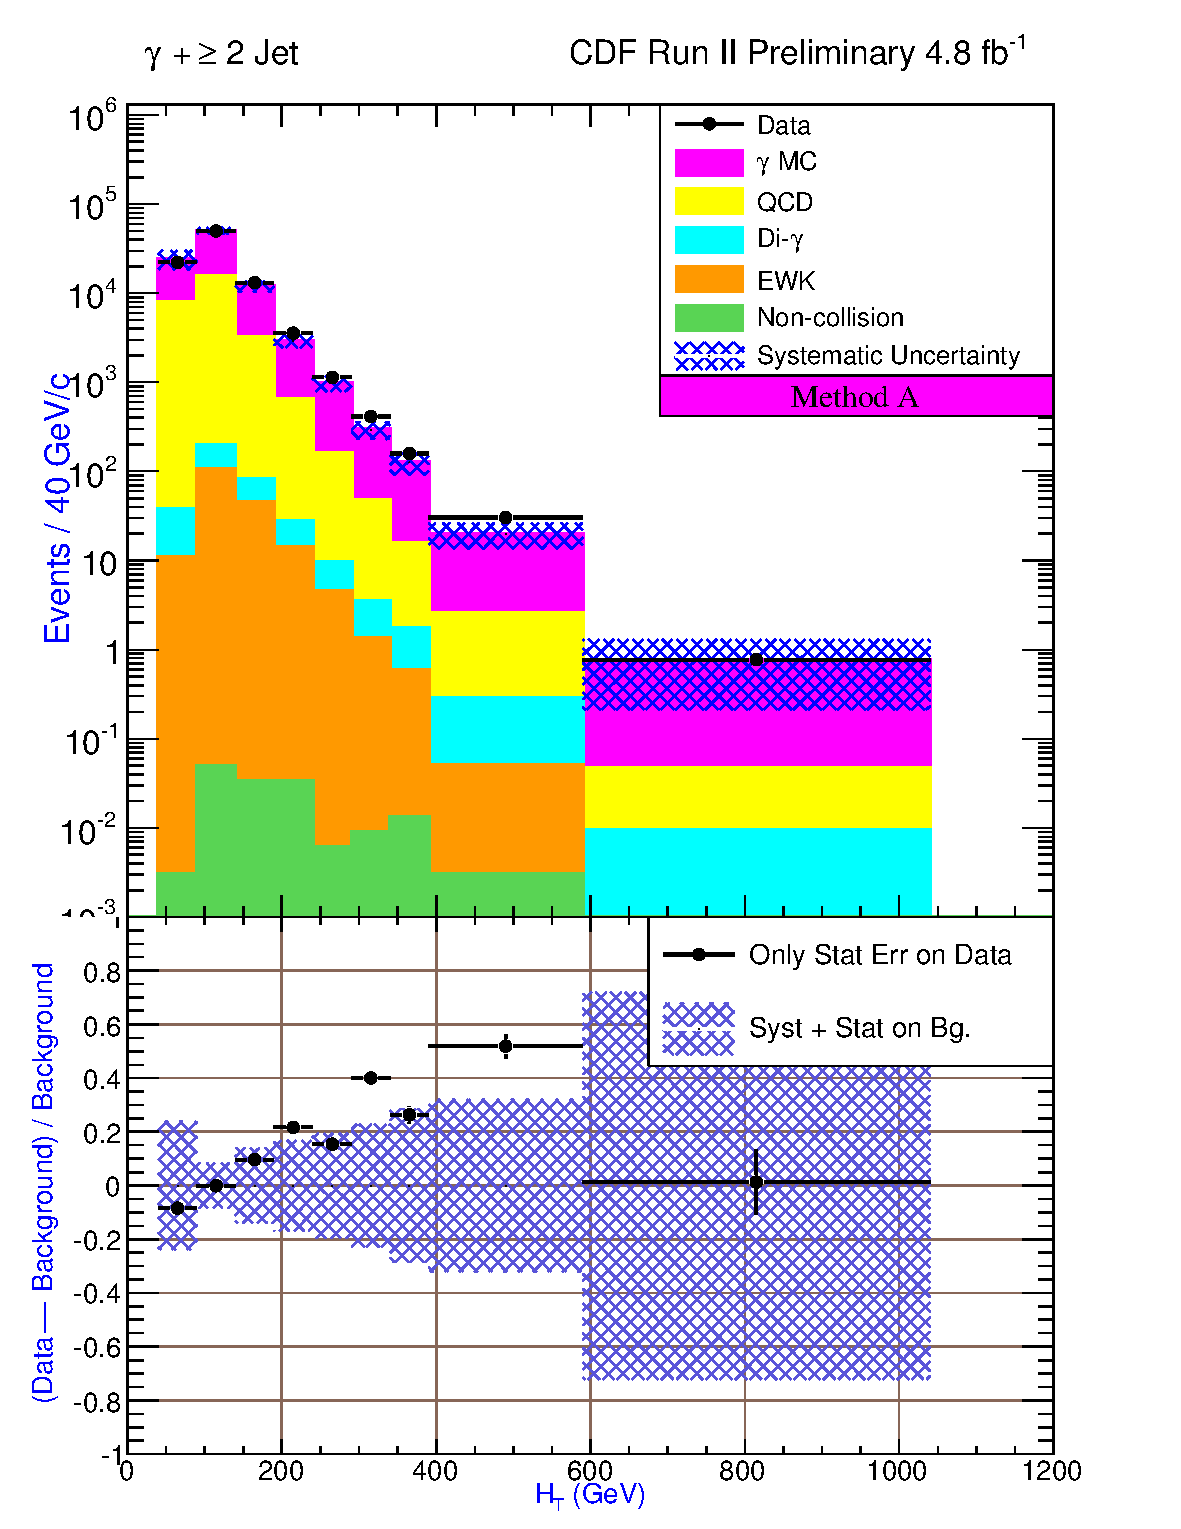
\includegraphics[keepaspectratio=true, scale=\figScale]{G30Jets_MtdA_plot2_Ht.pdf}}
\subfigure[]
{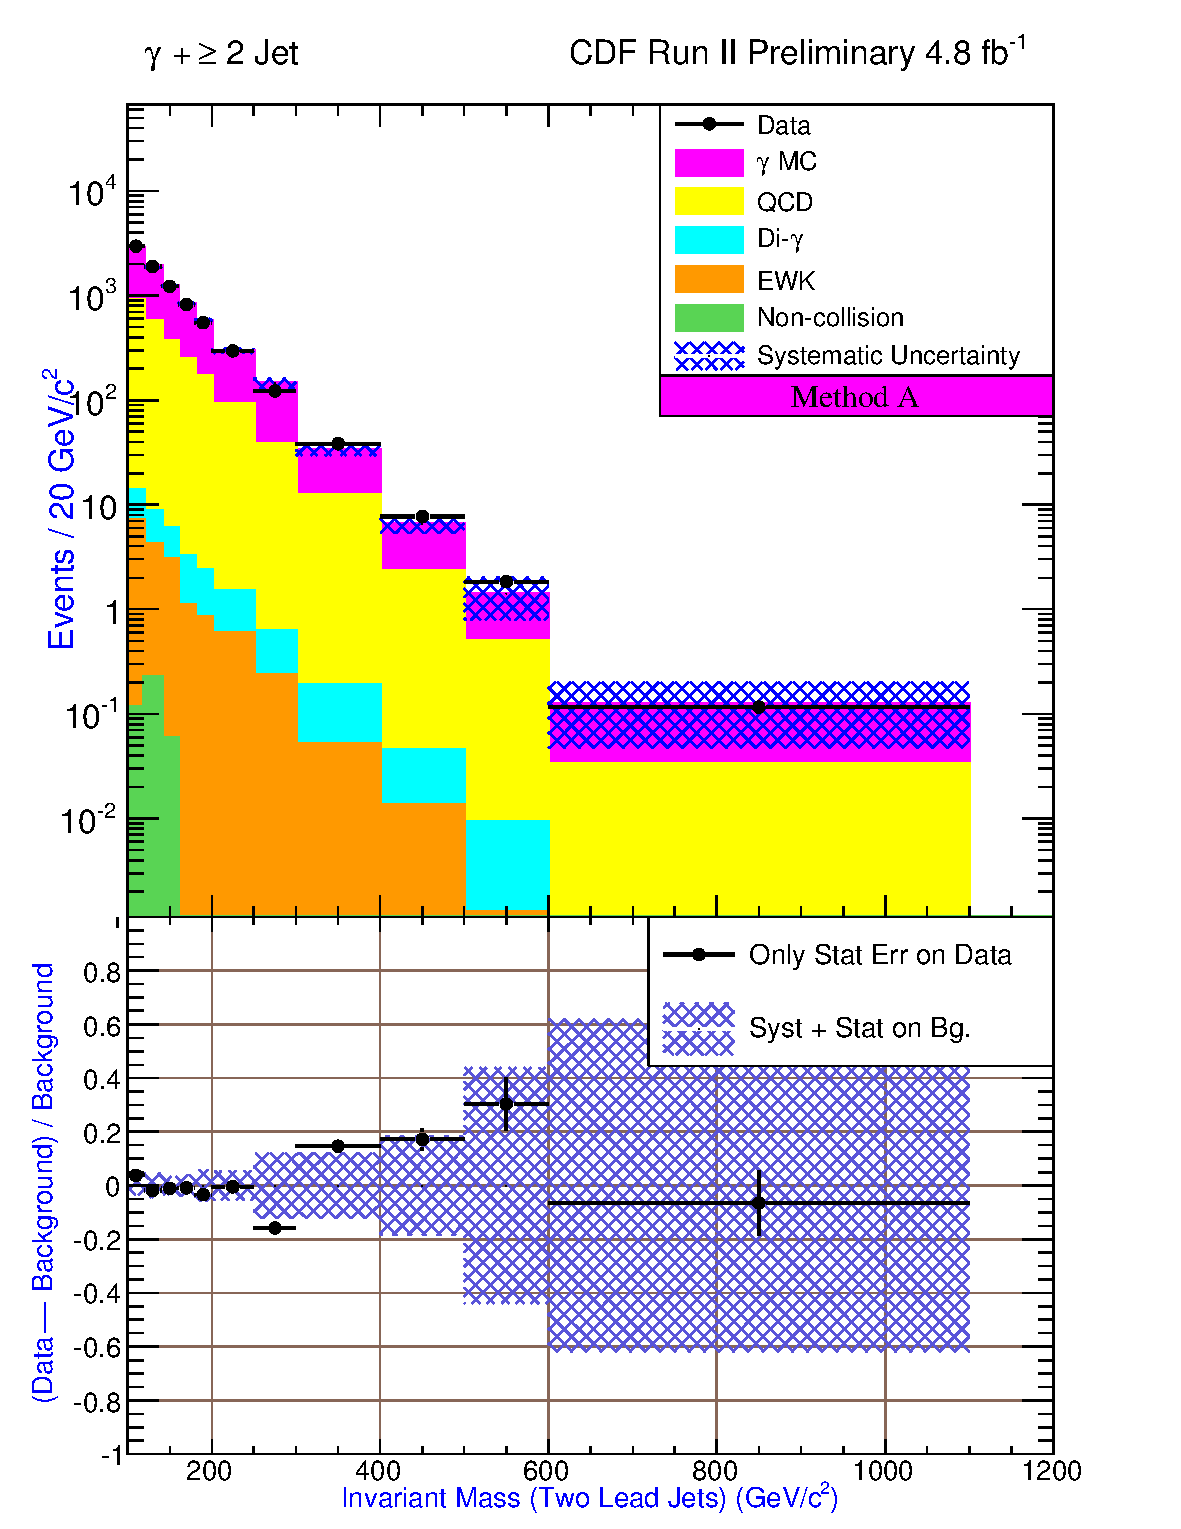
\includegraphics[keepaspectratio=true, scale=\figScale]{G30Jets_MtdA_plot2_InvMass_j1j2.pdf}}
\subfigure[]
{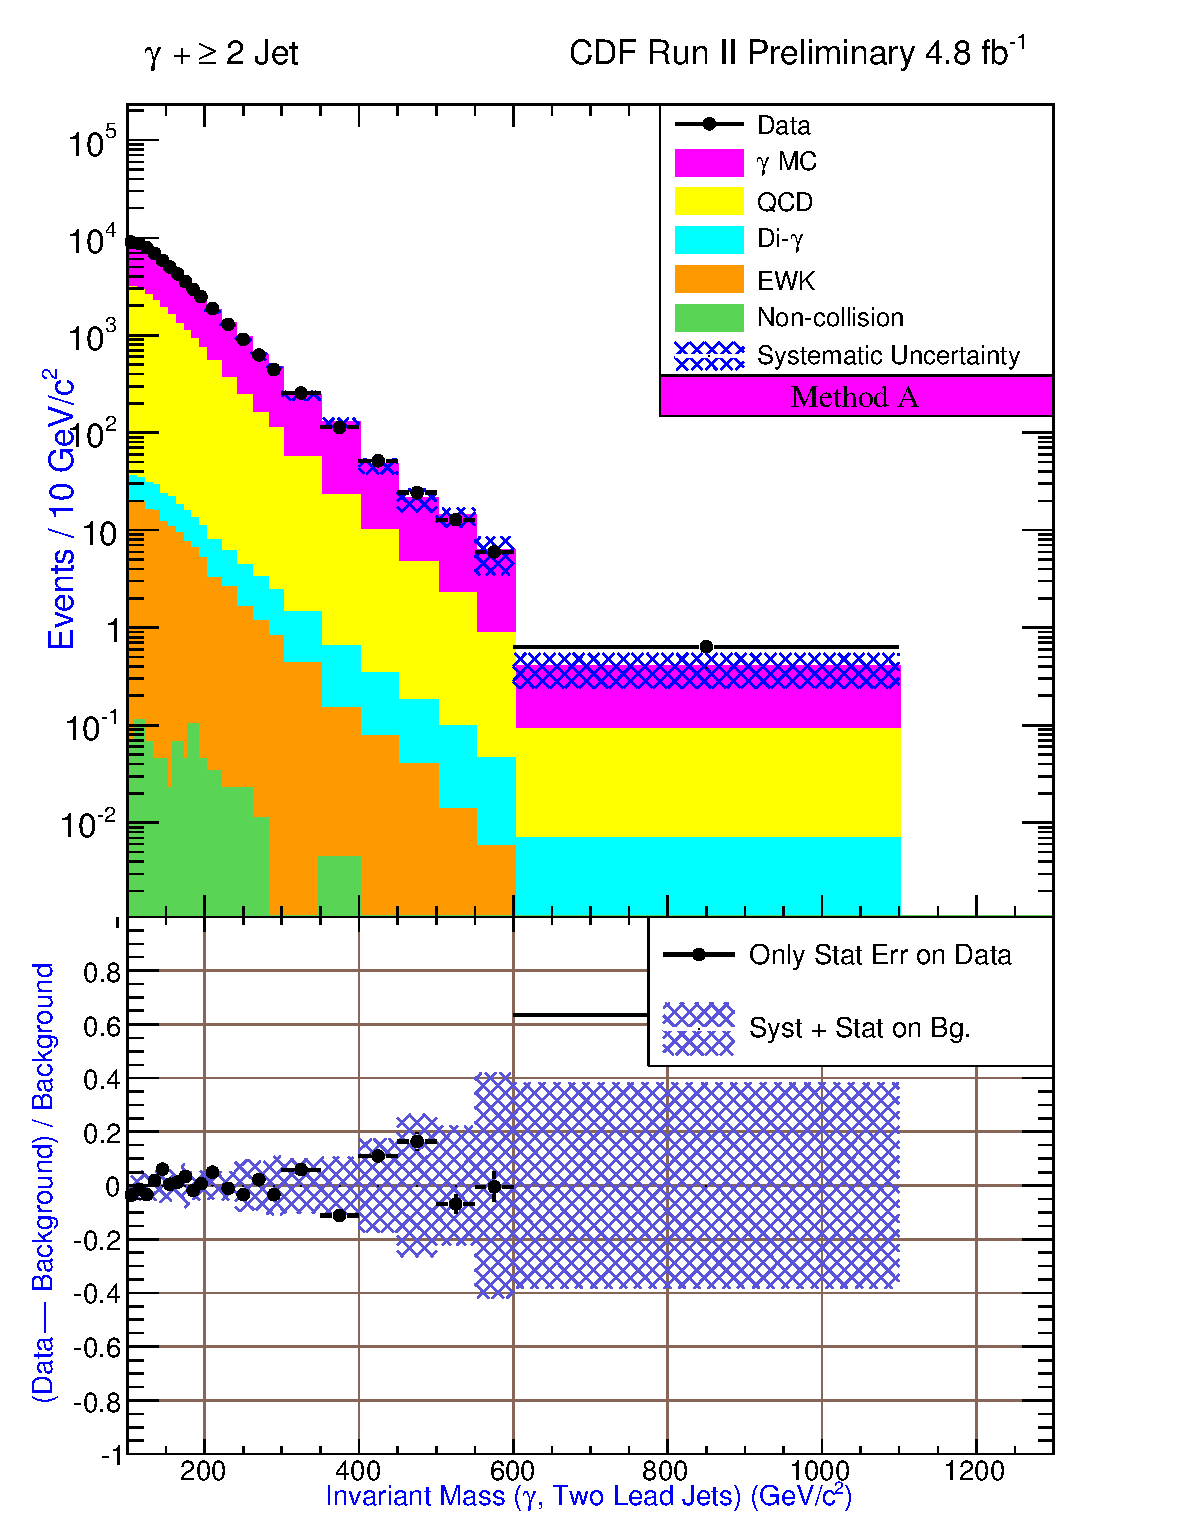
\includegraphics[keepaspectratio=true, scale=\figScale]{G30Jets_MtdA_plot2_InvMass_pj1j2.pdf}}
\subfigure[]
{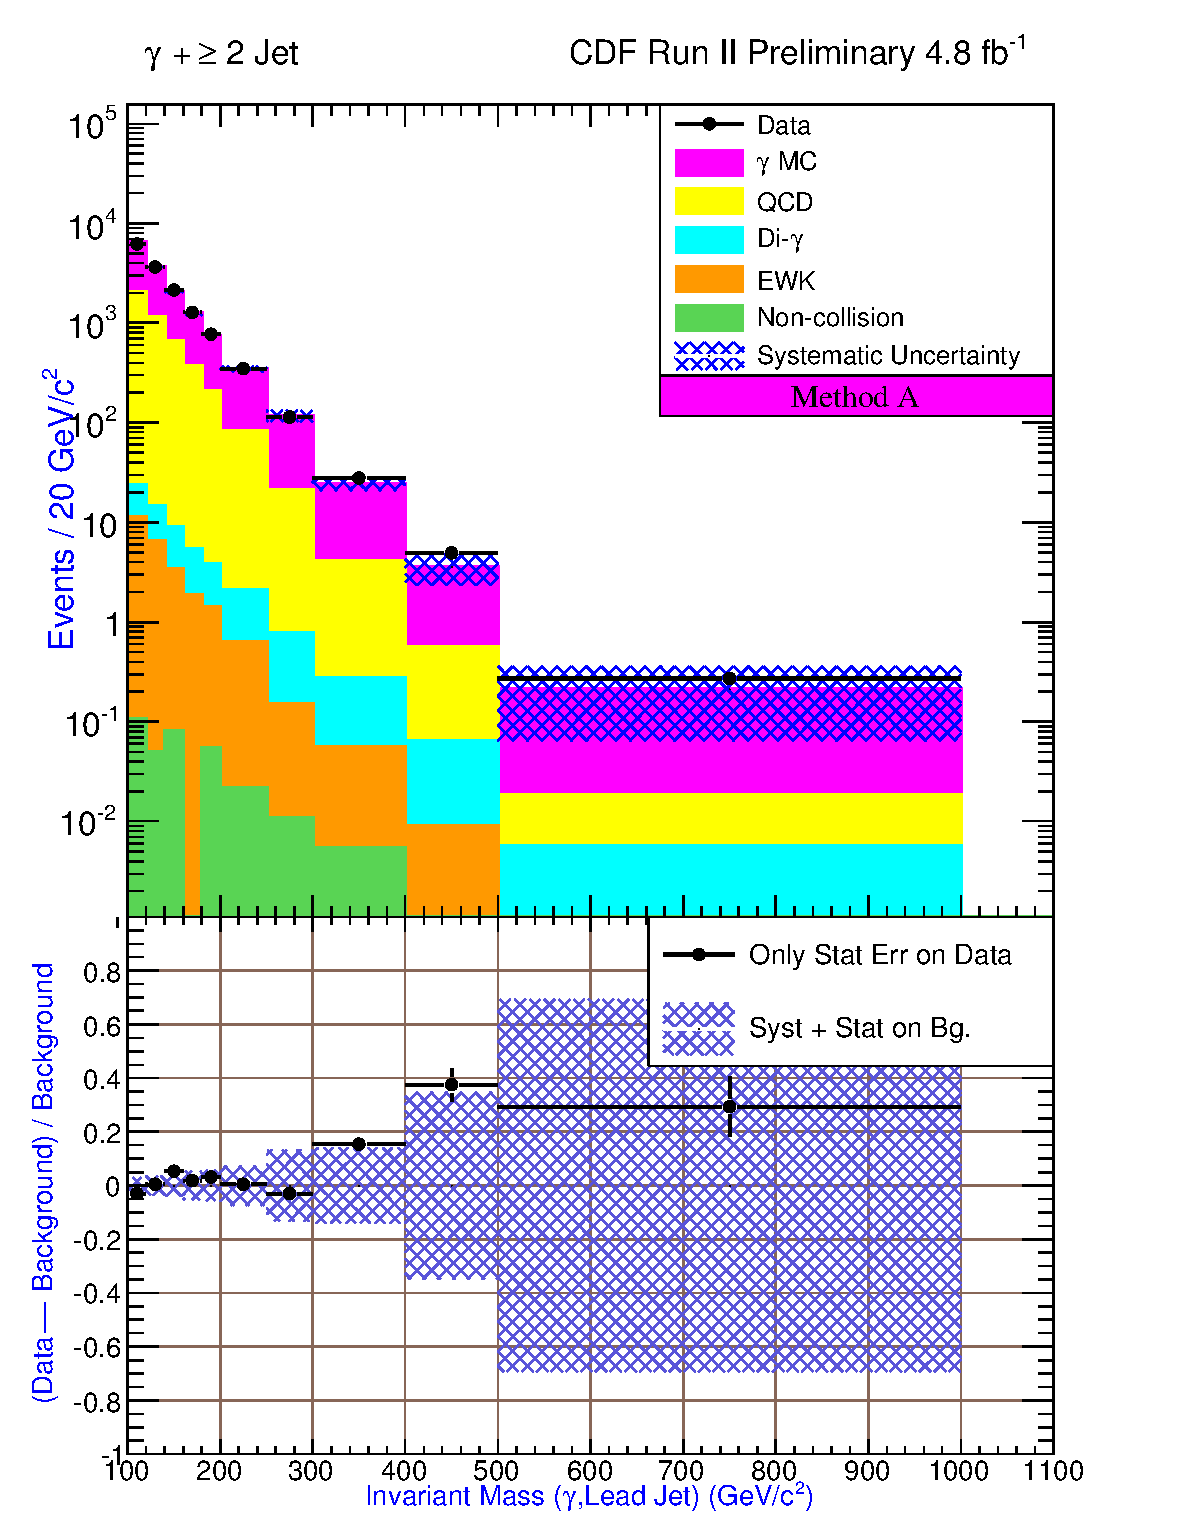
\includegraphics[keepaspectratio=true, scale=\figScale]{G30Jets_MtdA_plot2_InvMass_pj1.pdf}}
\label{fig:pjSetThree}
\end{figure*}
\clearpage

\begin{figure*}[h!]
\centering
\caption[Method A \phoonejet]{Kinematic distributions of \photwojet events using Method A.}
\subfigure[]
{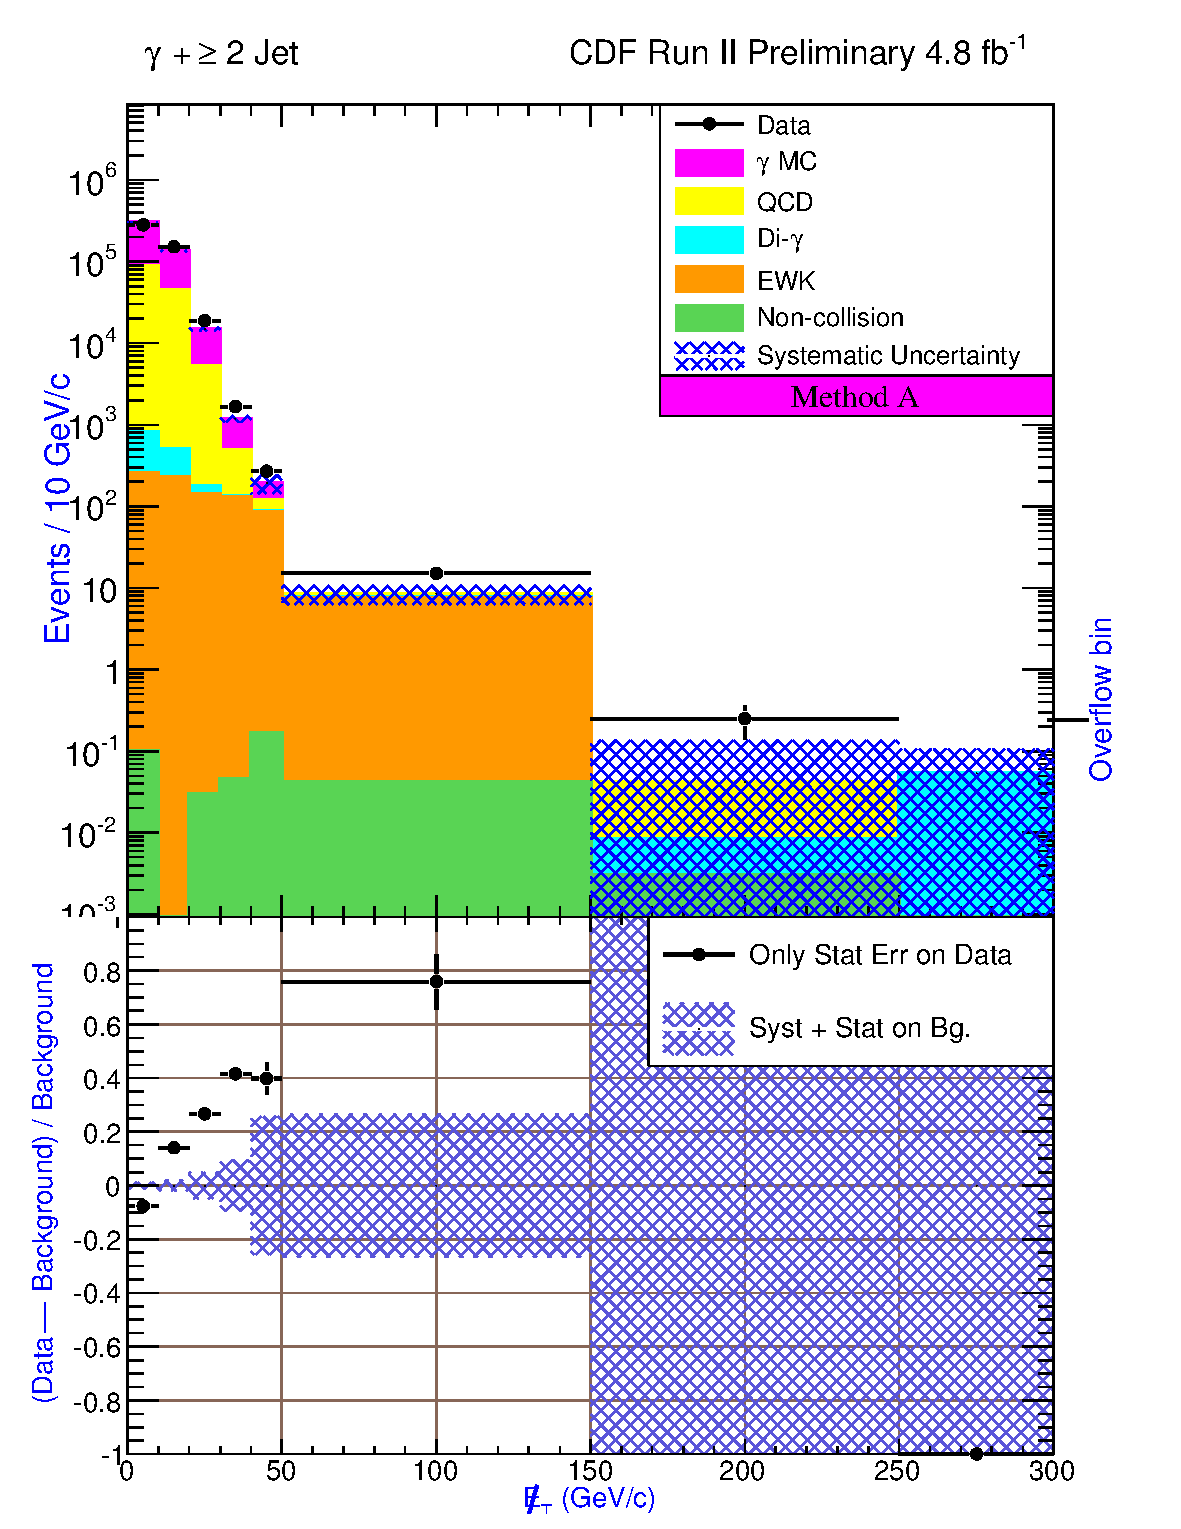
\includegraphics[keepaspectratio=true, scale=\figScale]{G30Jets_MtdA_plot2_Met.pdf}}
\label{fig:pjSetFour}
\end{figure*}
\clearpage

%%%%%%%%%%%%%%%%%%%%%%%%%%%%%% METHOD A: G30 JETS+MET>20
\begin{figure*}[h!]
\centering
\caption[Method A \phoonejet]{Kinematic distributions of \phoonejet + \met$>$~20~GeV events using \mbox{Method A}. See Section~\ref{sec:PrelResults} for a description of the elements in these distributions.}
\subfigure[]
{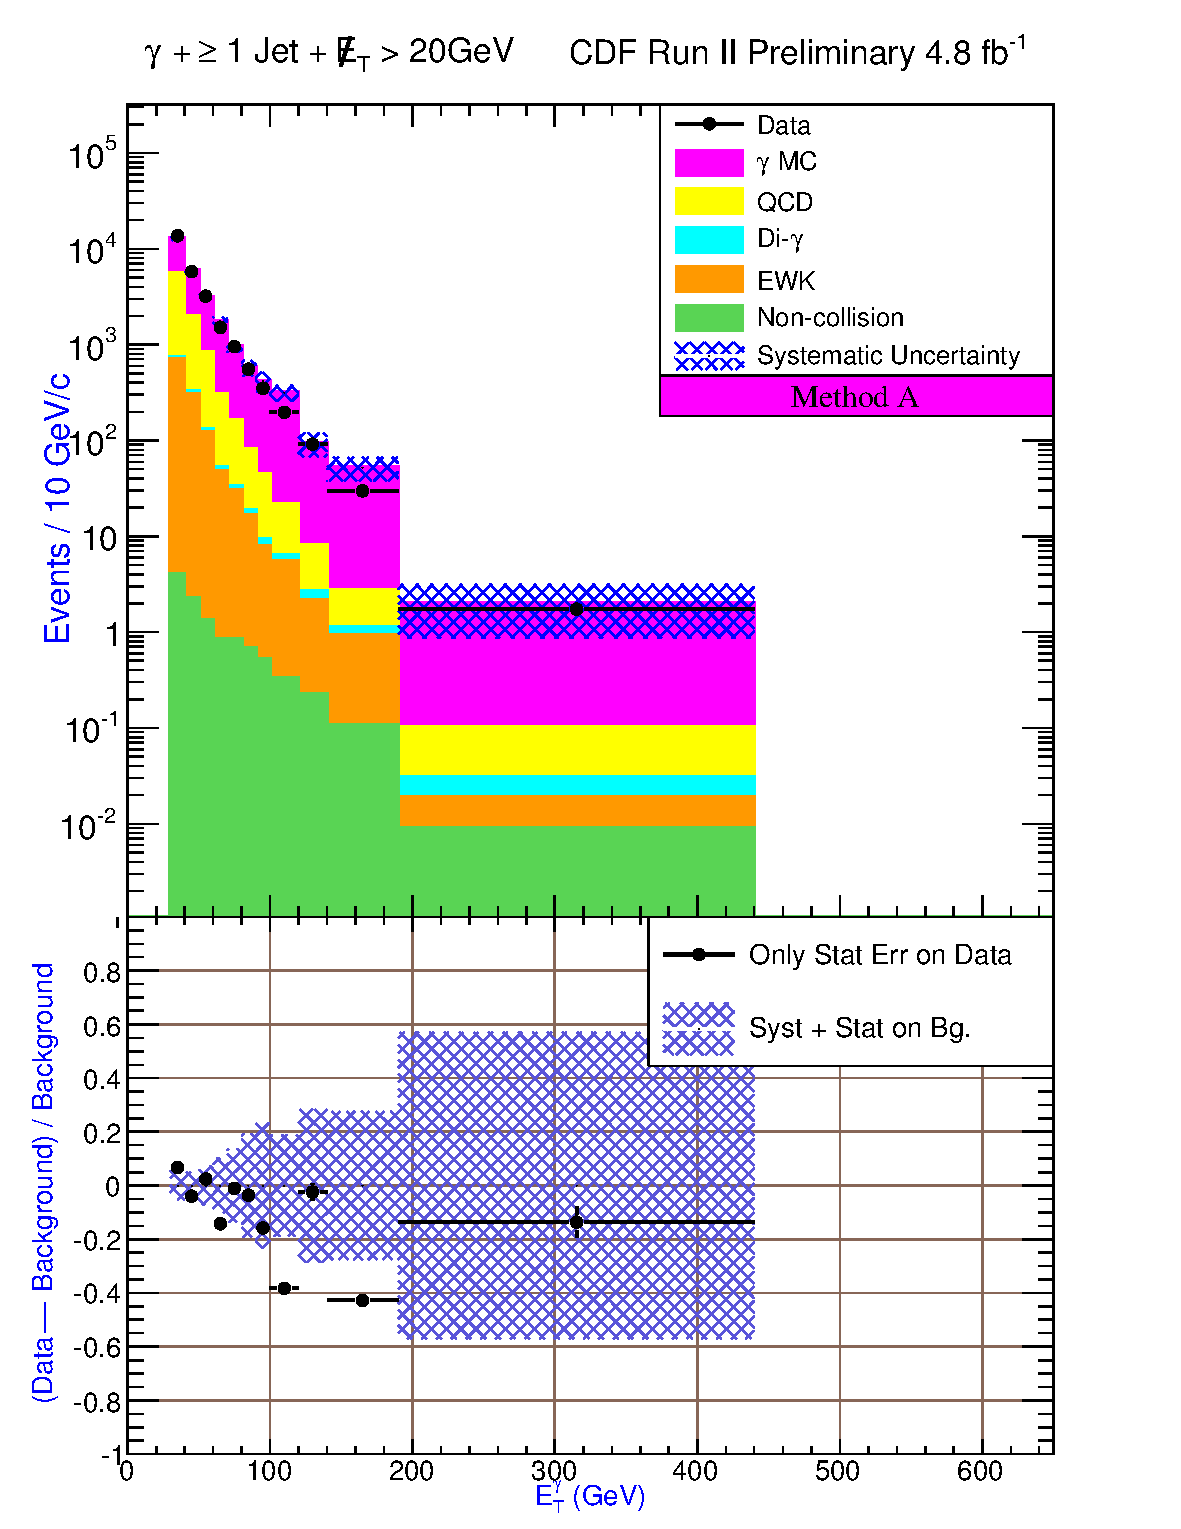
\includegraphics[keepaspectratio=true, scale=\figScale]{G30JetsMet20_MtdA_plot1_Et_pho.pdf}}
\subfigure[]
{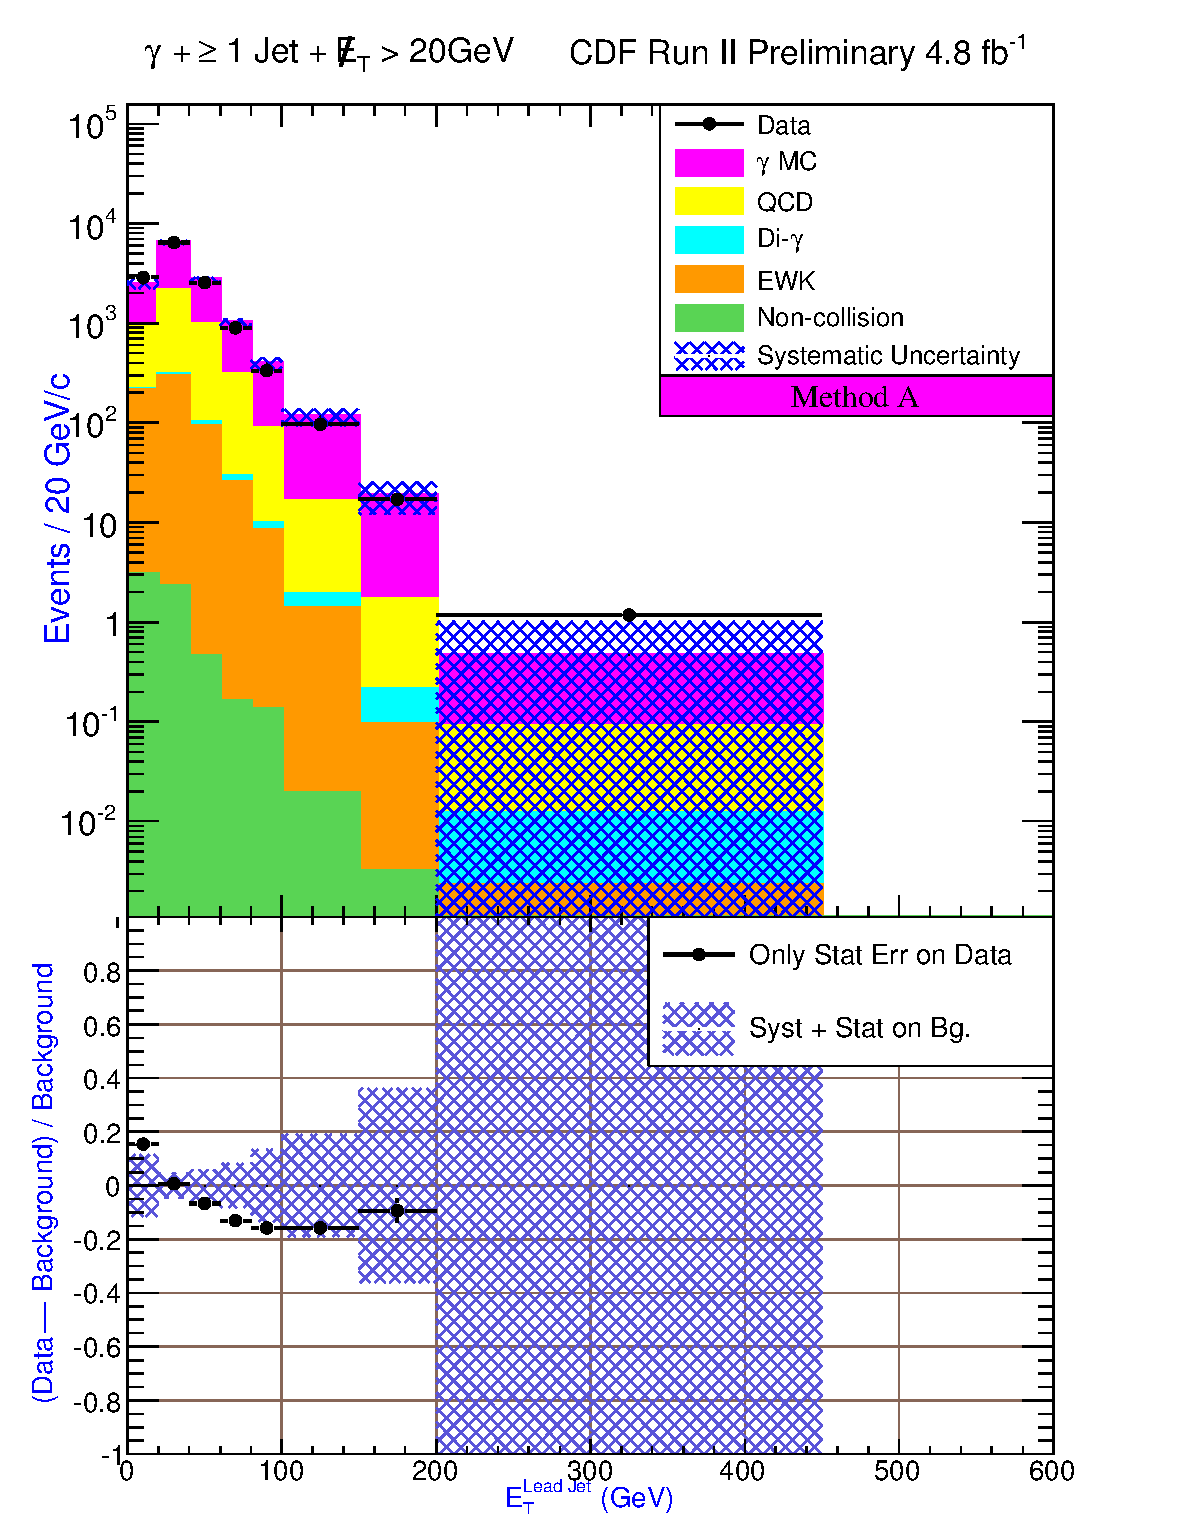
\includegraphics[keepaspectratio=true, scale=\figScale]{G30JetsMet20_MtdA_plot1_Et_j1.pdf}
}

\subfigure[]
{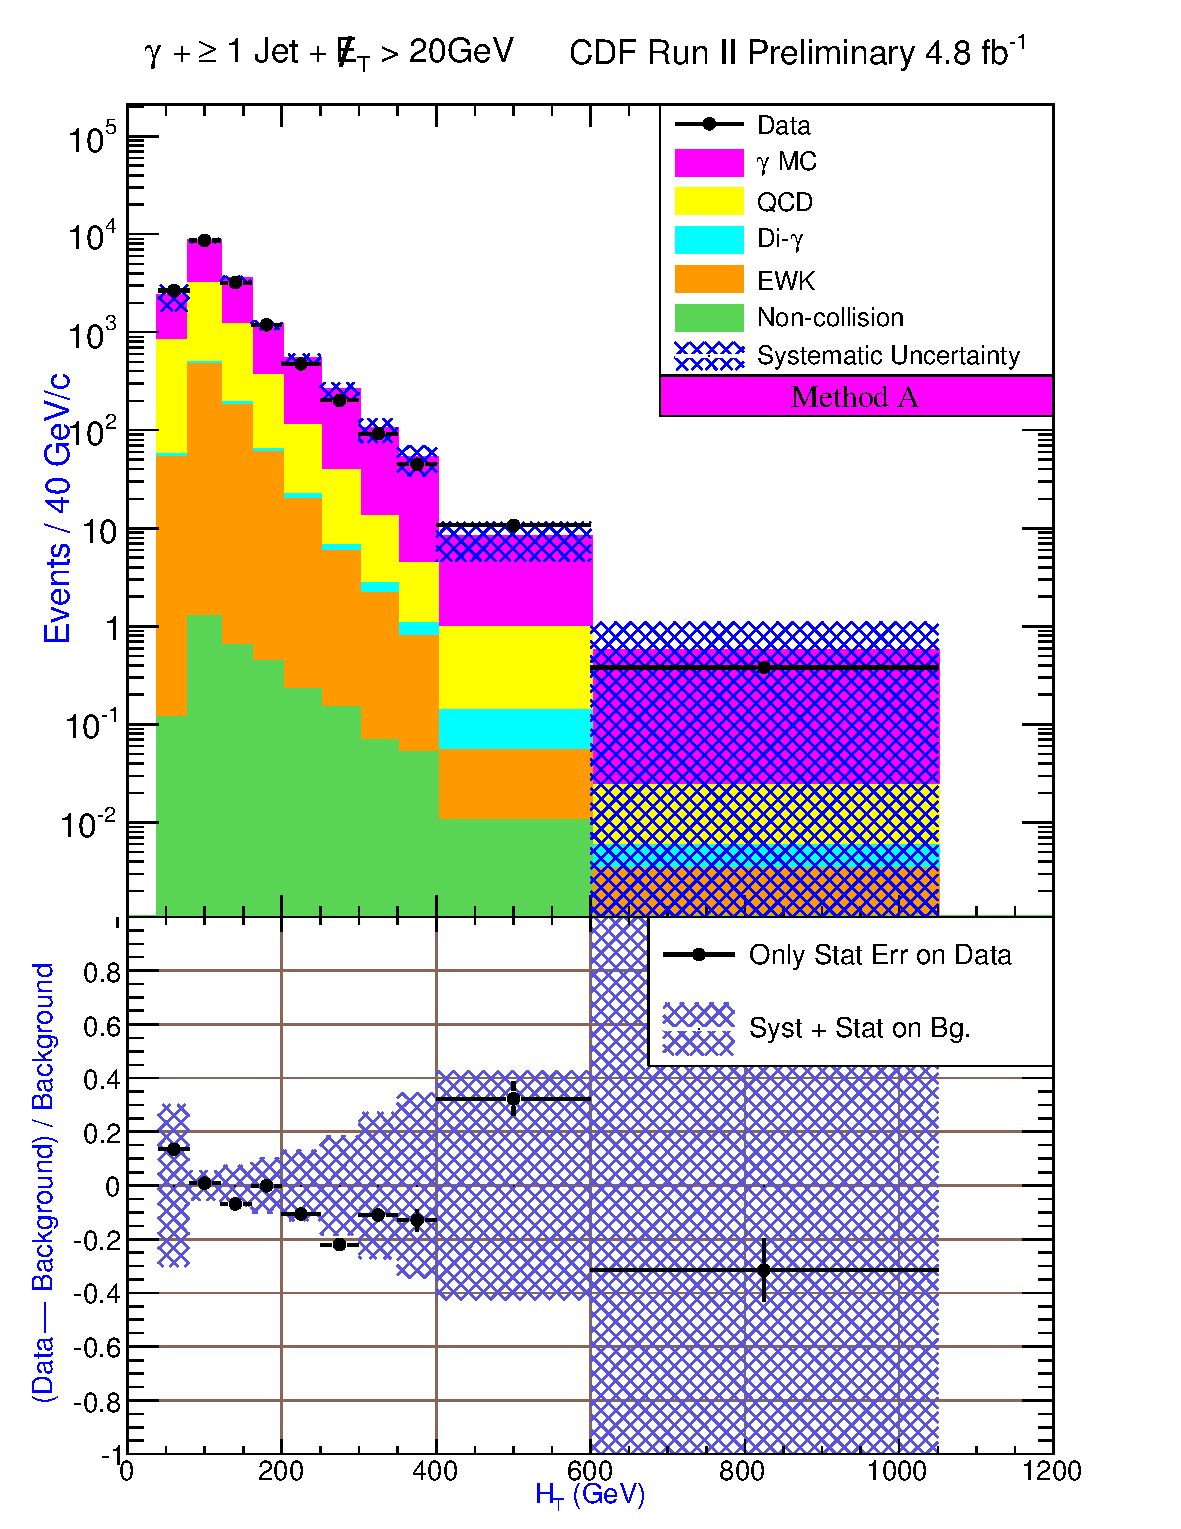
\includegraphics[keepaspectratio=true, scale=\figScale]{G30JetsMet20_MtdA_plot1_Ht.pdf}}
\subfigure[]
{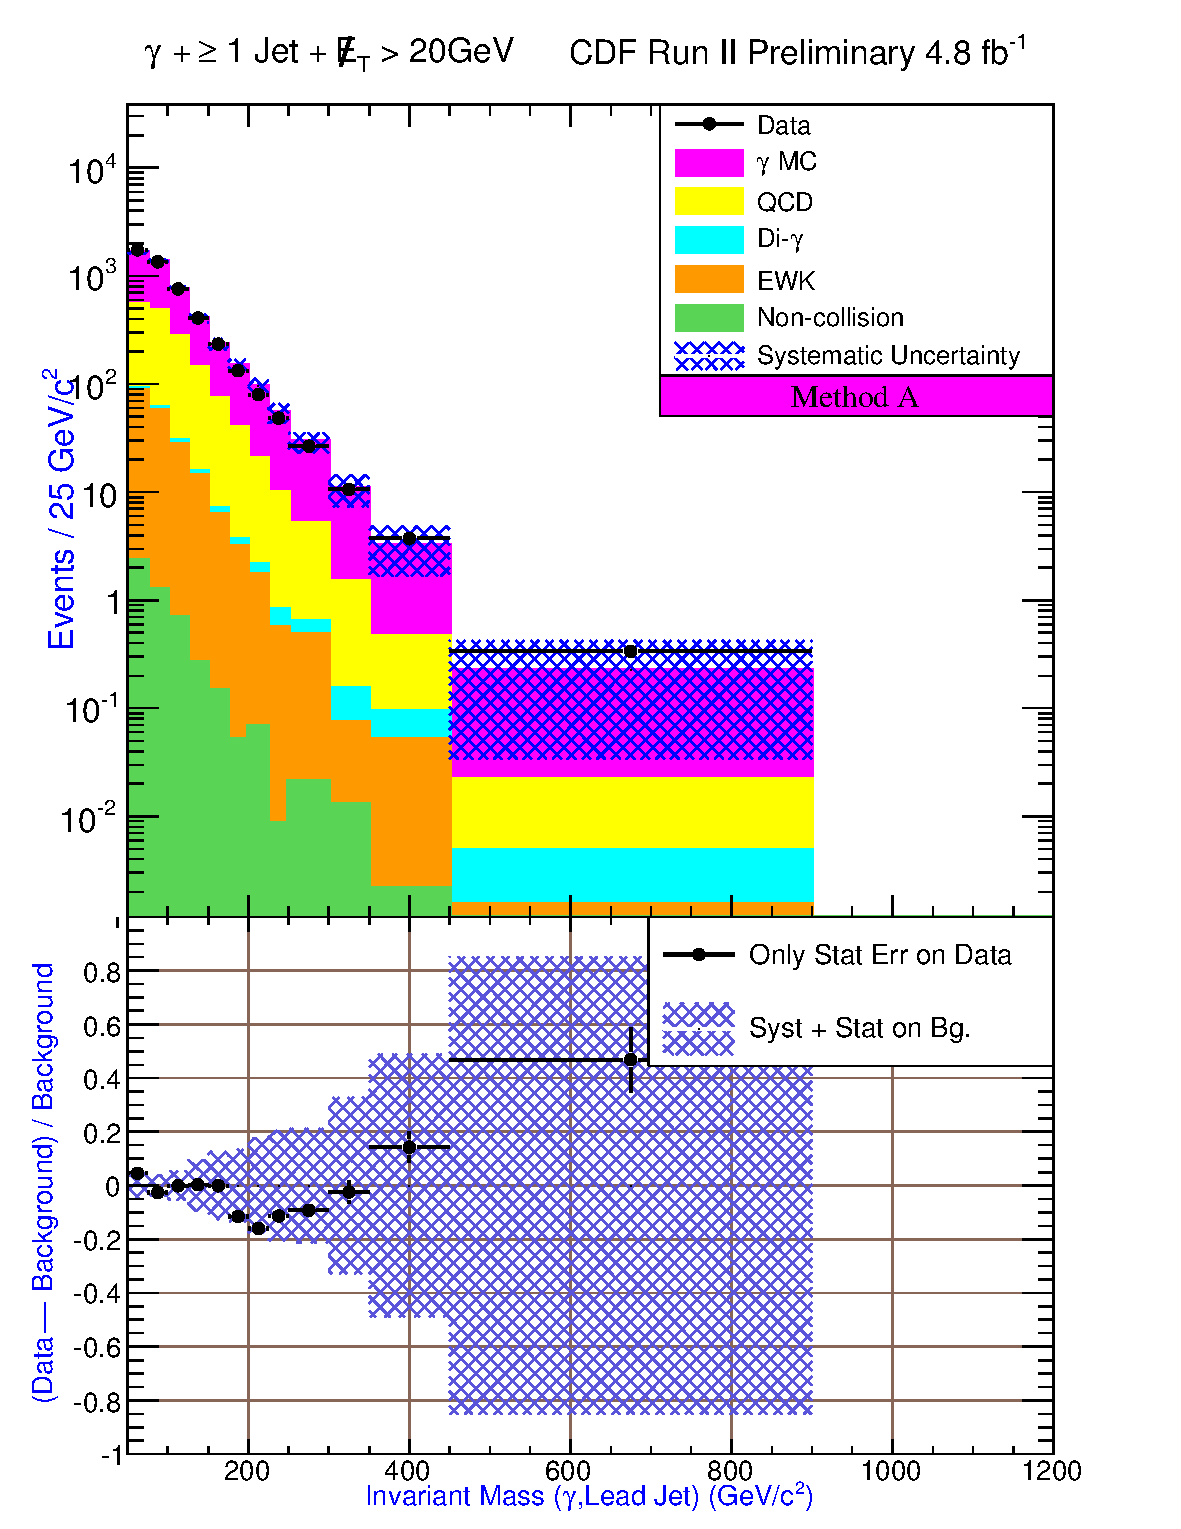
\includegraphics[keepaspectratio=true, scale=\figScale]{G30JetsMet20_MtdA_plot1_InvMass_pj1.pdf}}
\label{fig:pjMetSetOne}
\end{figure*}
\clearpage

\begin{figure*}[h!]
\centering
\caption[Method A \phoonejet]{Kinematic distributions of \phoonejet + \met$>$~20~GeV (top) and \photwojet + \met$>$~20~GeV (bottom) events using Method A. See Section~\ref{sec:PrelResults} for a description of the elements in these distributions.}
\subfigure[]
{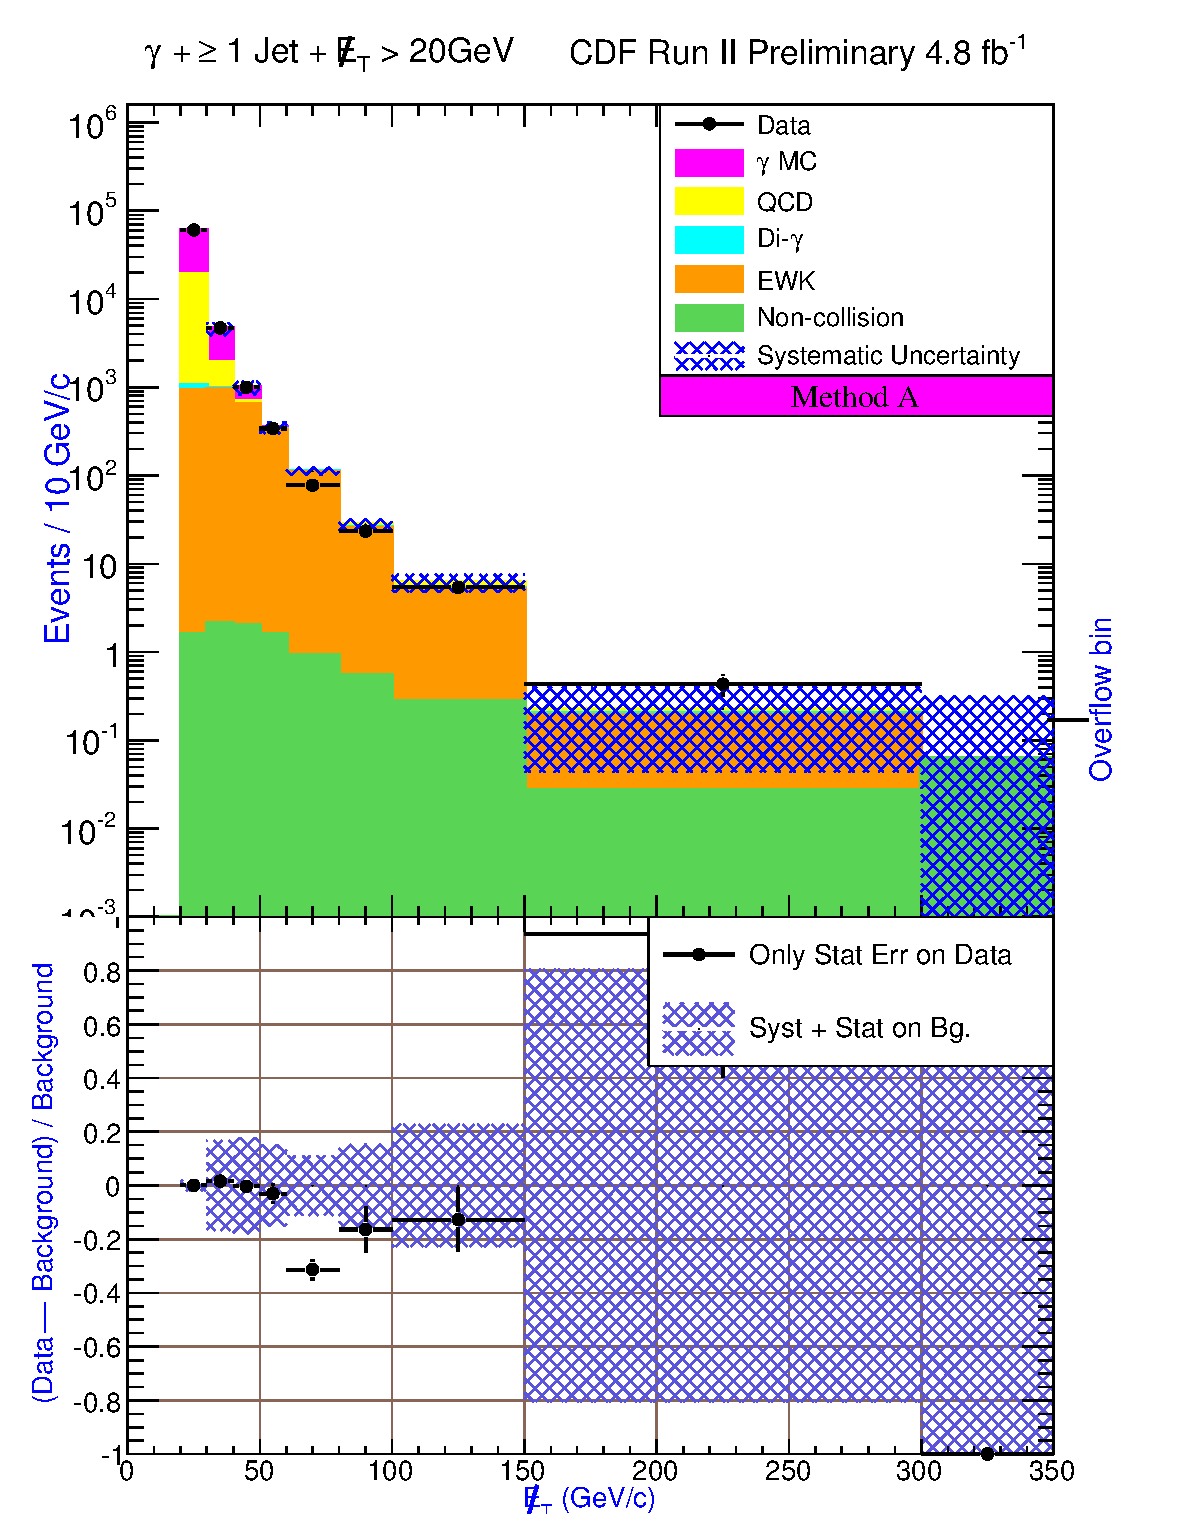
\includegraphics[keepaspectratio=true, scale=\figScale]{G30JetsMet20_MtdA_plot1_Met.pdf}}
\subfigure[]
{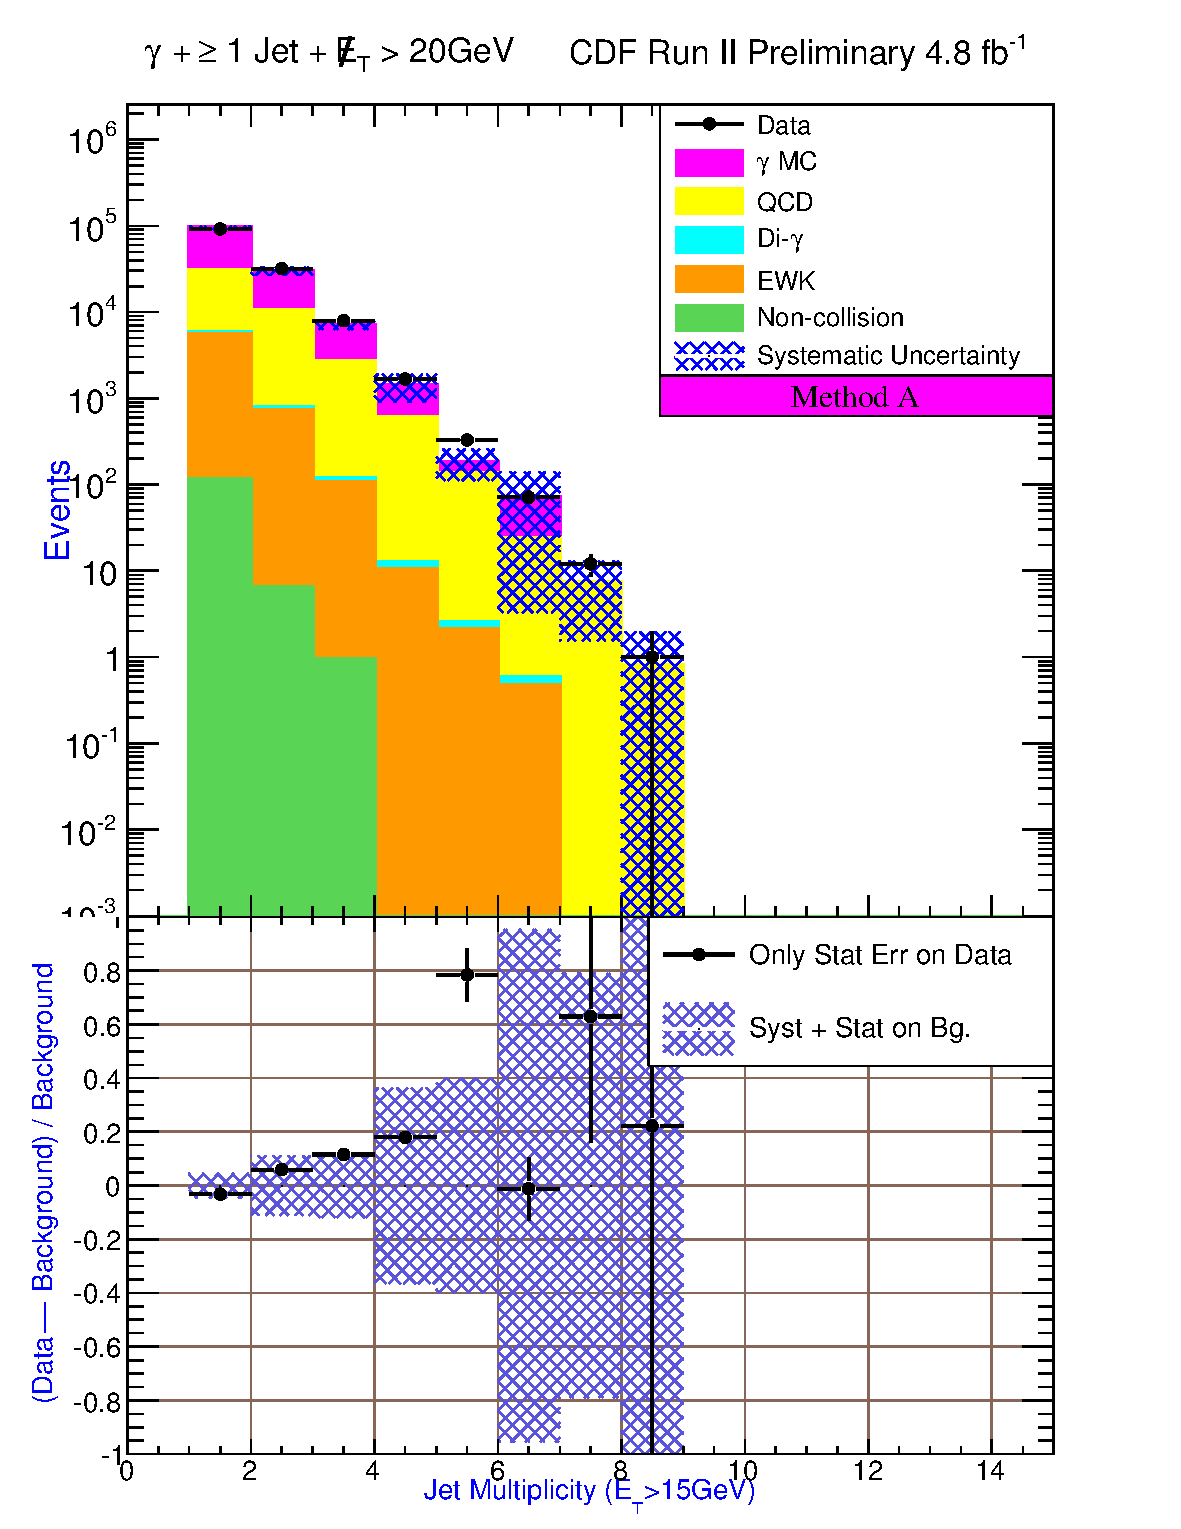
\includegraphics[keepaspectratio=true, scale=\figScale]{G30JetsMet20_MtdA_plot1_NJet.pdf}}
\subfigure[]
{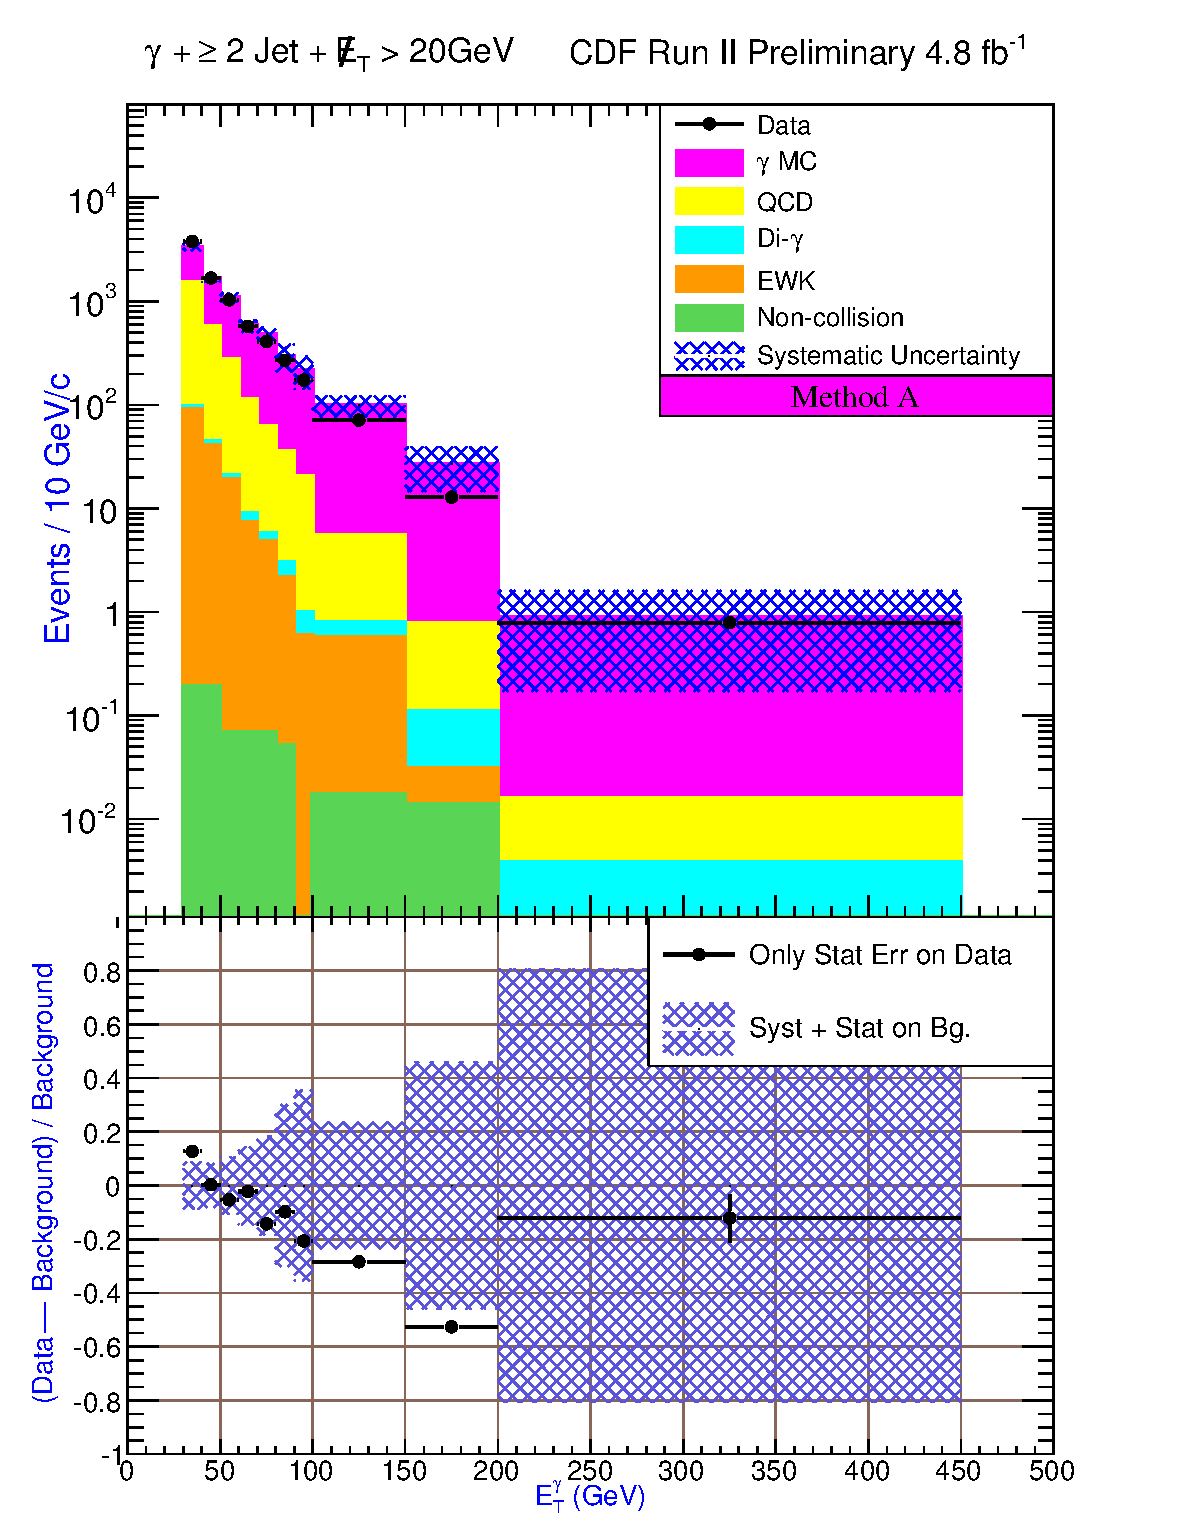
\includegraphics[keepaspectratio=true, scale=\figScale]{G30JetsMet20_MtdA_plot2_Et_pho.pdf}}
\subfigure[]
{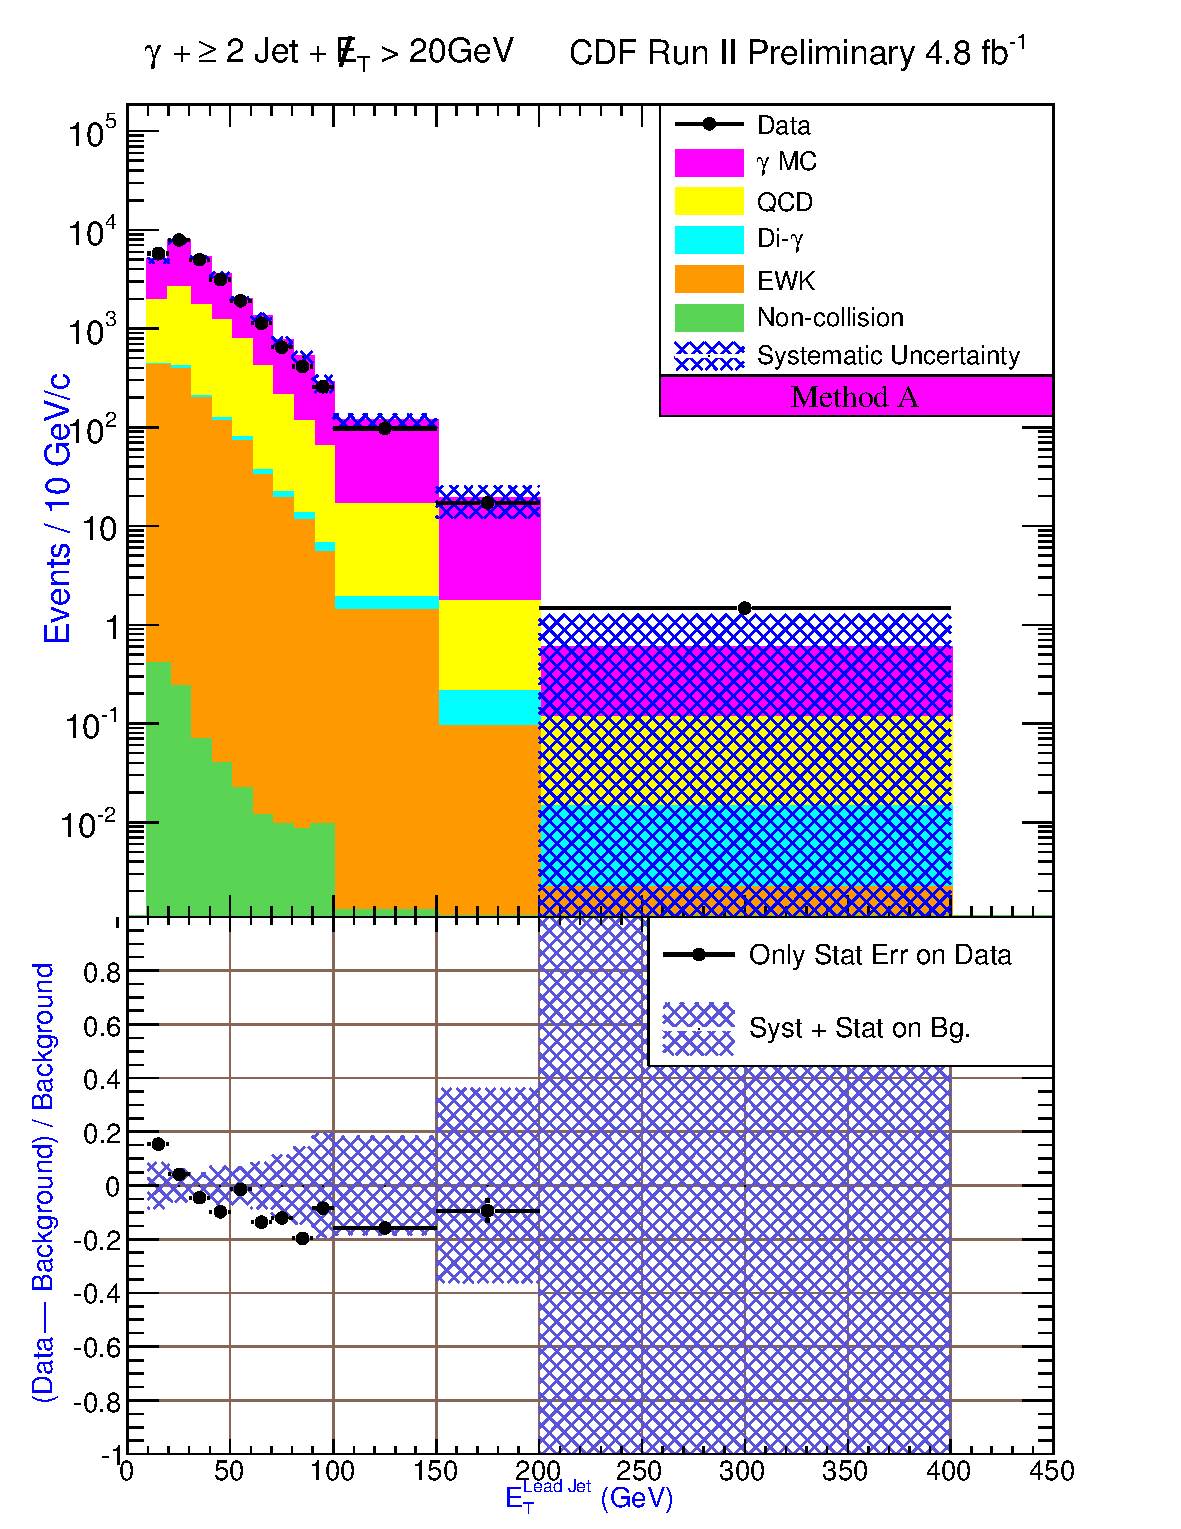
\includegraphics[keepaspectratio=true, scale=\figScale]{G30JetsMet20_MtdA_plot2_Et_j1.pdf}}
\label{fig:pjMetSetTwo}
\end{figure*}
\clearpage

\begin{figure*}[h!]
\centering
\caption[Method A \photwojet]{Kinematic distributions of \photwojet + \met$>$~20~GeV events using \mbox{Method A}. See Section~\ref{sec:PrelResults} for a description of the elements in these distributions.}
\subfigure[]
{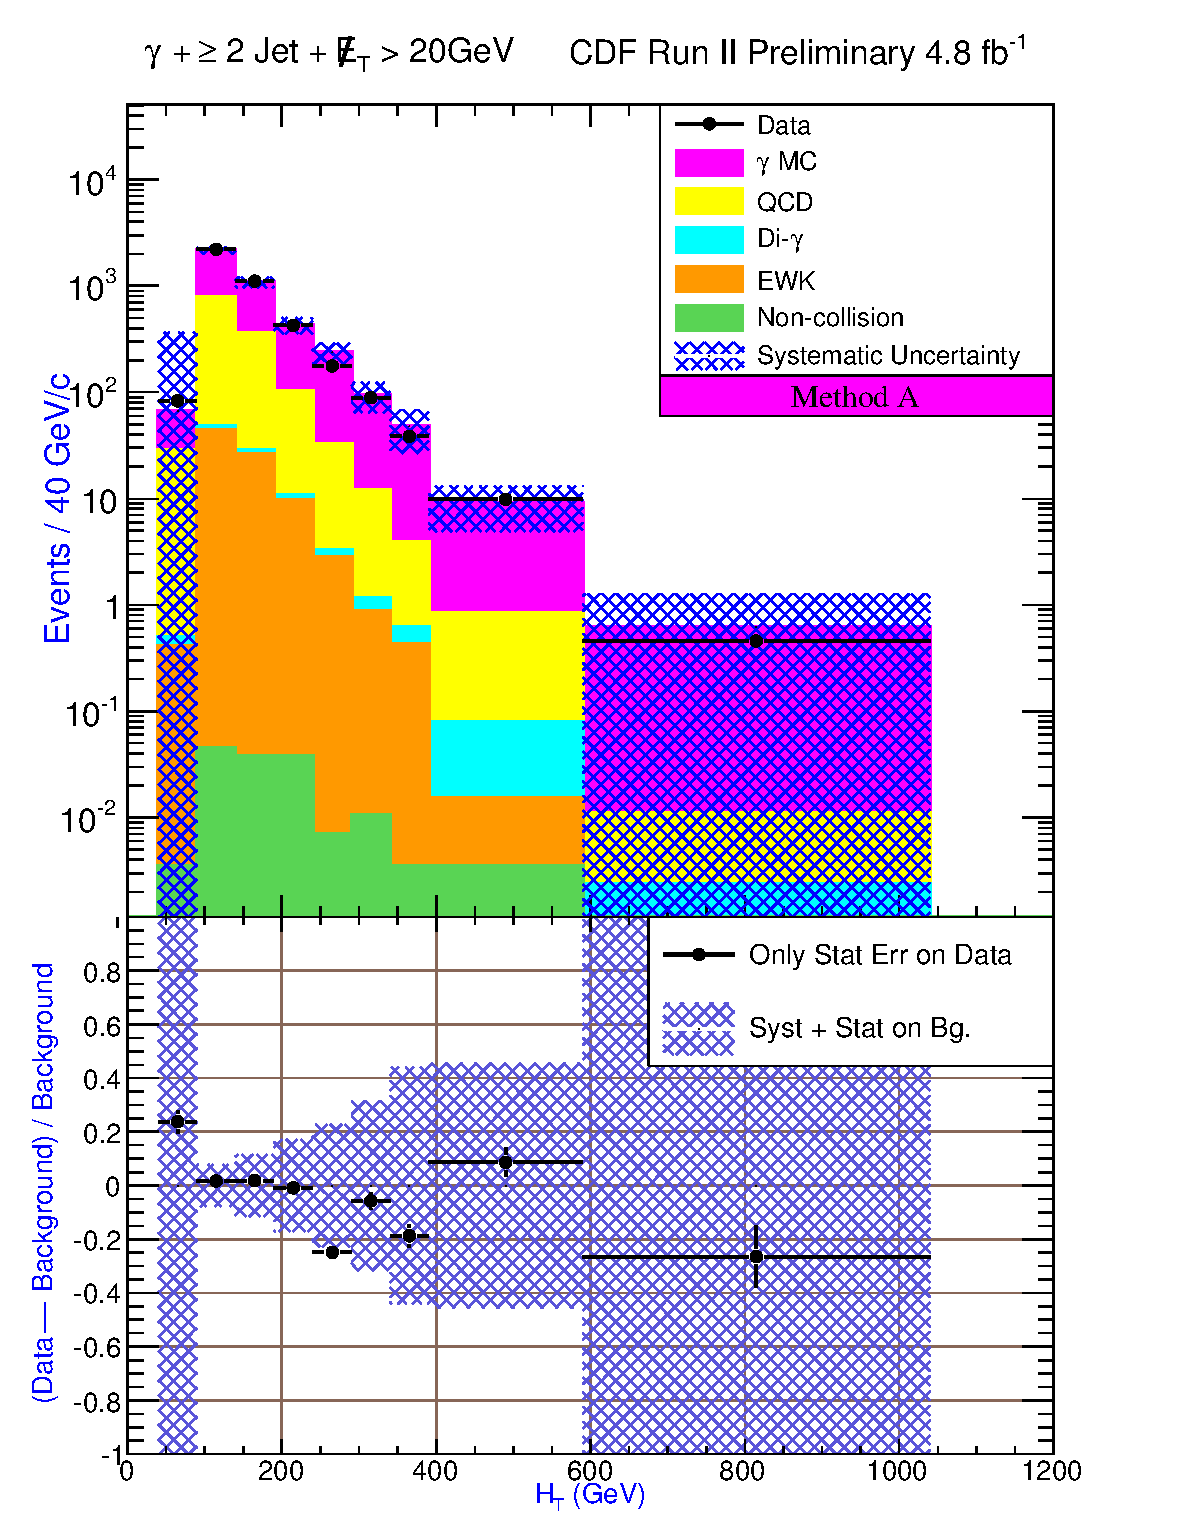
\includegraphics[keepaspectratio=true, scale=\figScale]{G30JetsMet20_MtdA_plot2_Ht.pdf}}
\subfigure[]
{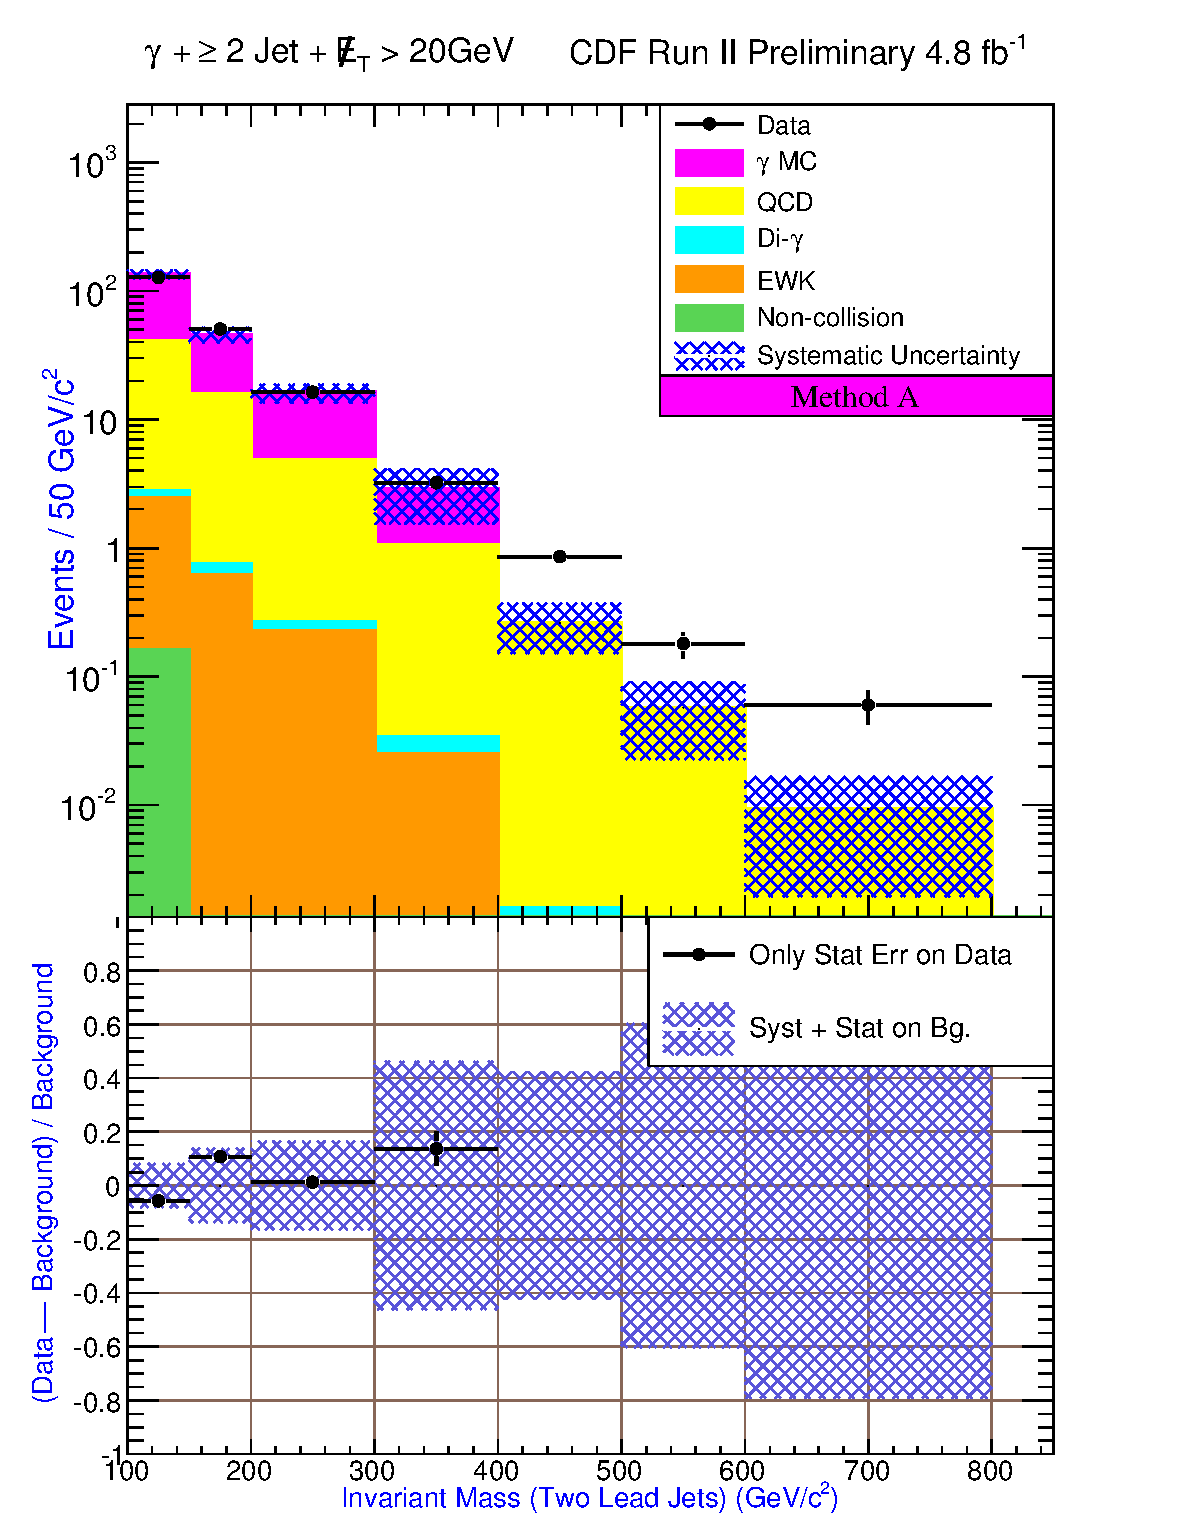
\includegraphics[keepaspectratio=true, scale=\figScale]{G30JetsMet20_MtdA_plot2_InvMass_j1j2.pdf}}
\subfigure[]
{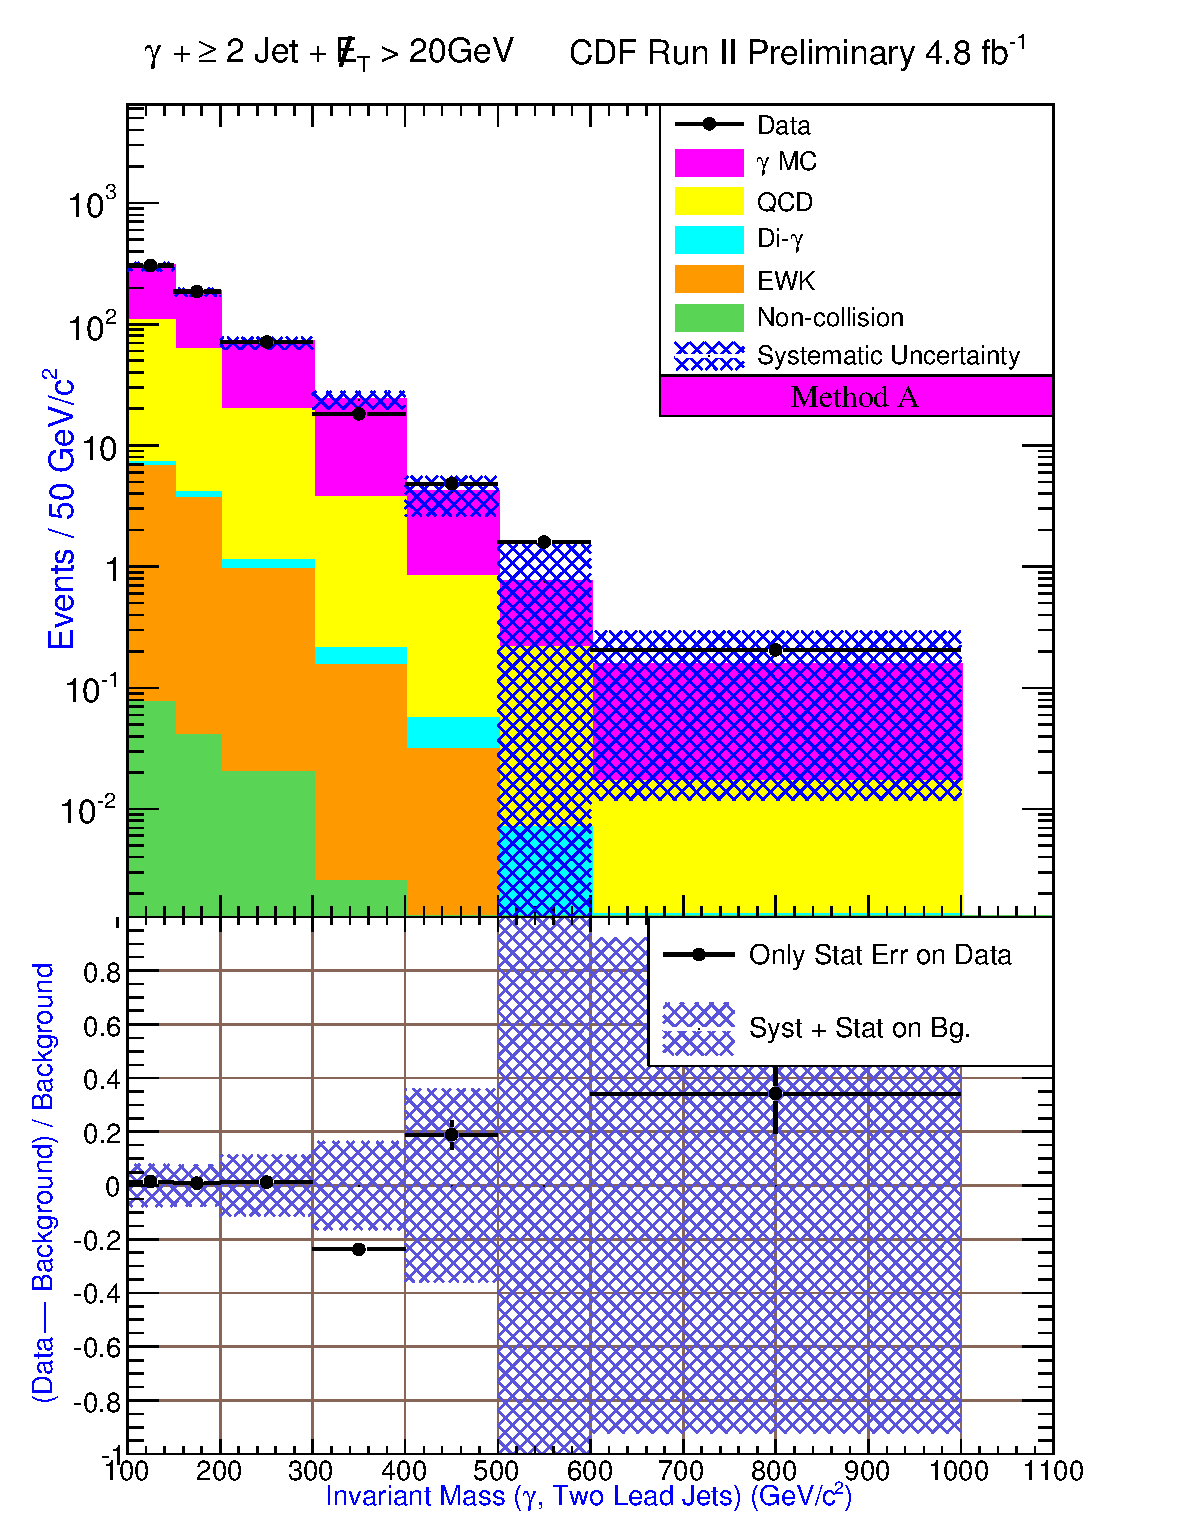
\includegraphics[keepaspectratio=true, scale=\figScale]{G30JetsMet20_MtdA_plot2_InvMass_pj1j2.pdf}}
\subfigure[]
{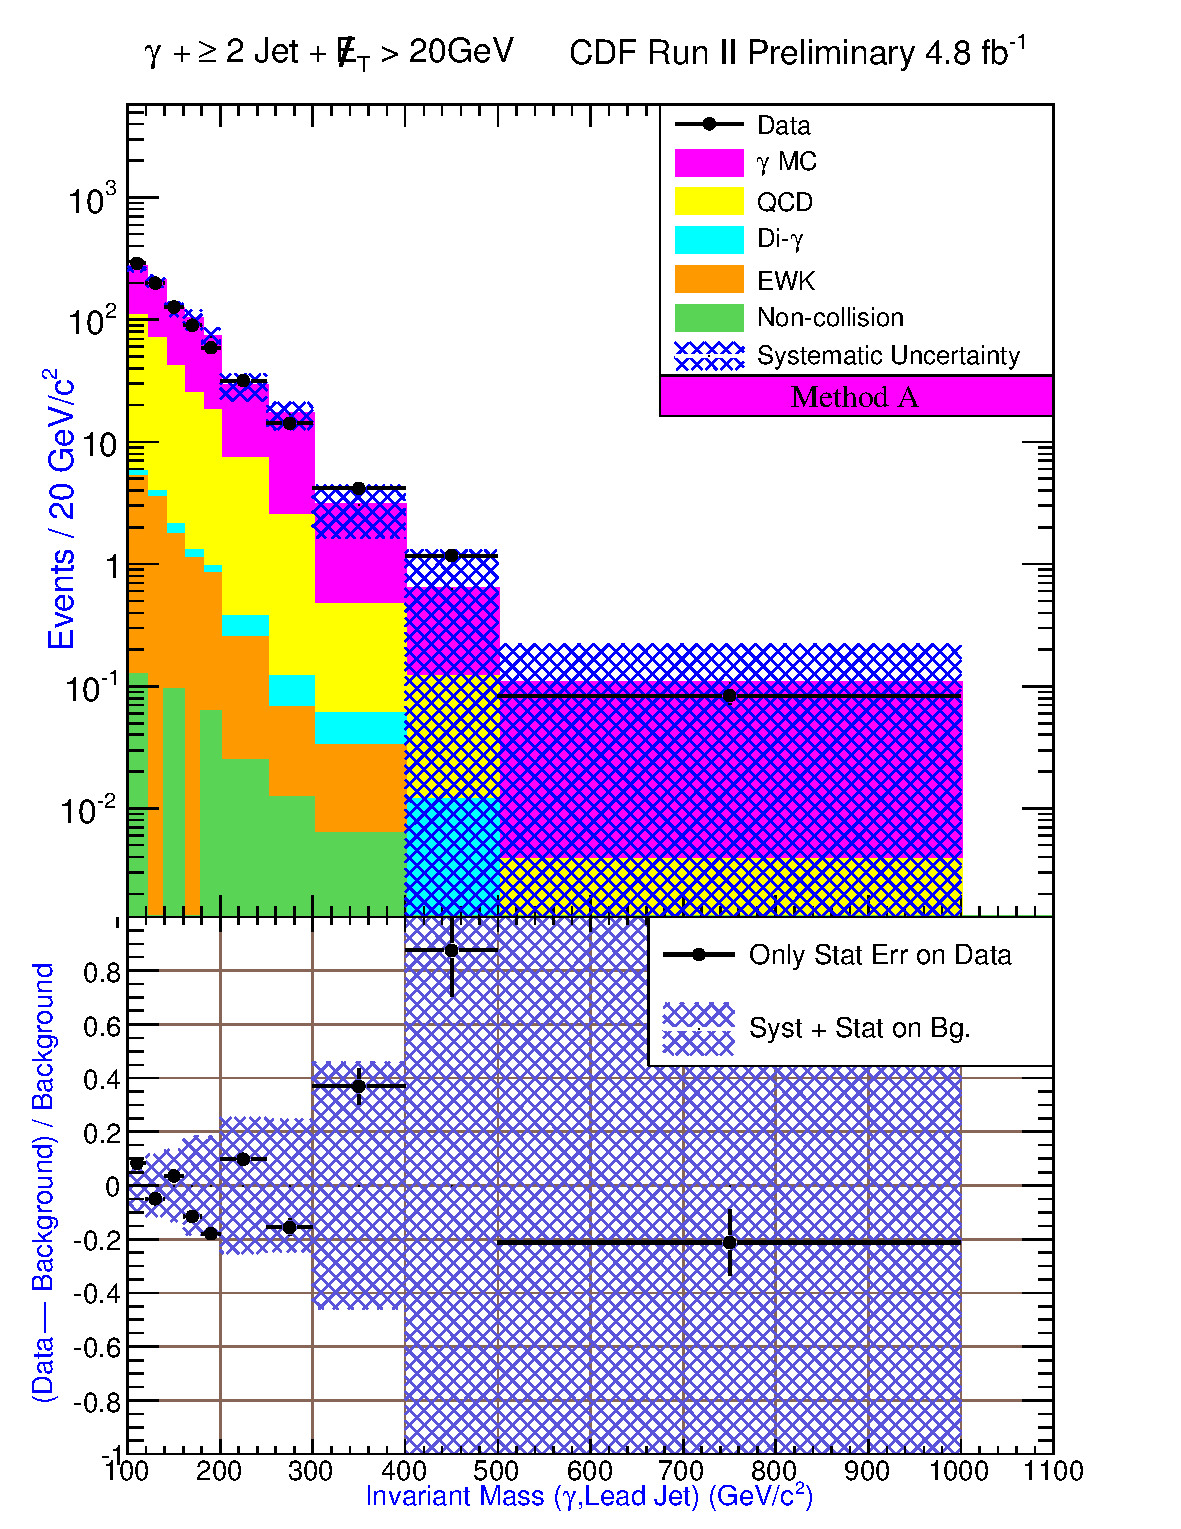
\includegraphics[keepaspectratio=true, scale=\figScale]{G30JetsMet20_MtdA_plot2_InvMass_pj1.pdf}}
\label{fig:pjMetSetThree}
\end{figure*}
\clearpage

\begin{figure*}[h!]
\centering
\caption[Method A \photwojet]{Kinematic distributions of \photwojet + \met$>$~20~GeV events using \mbox{Method A}. See Section~\ref{sec:PrelResults} for a description of the elements in these distributions.}
\subfigure[]
{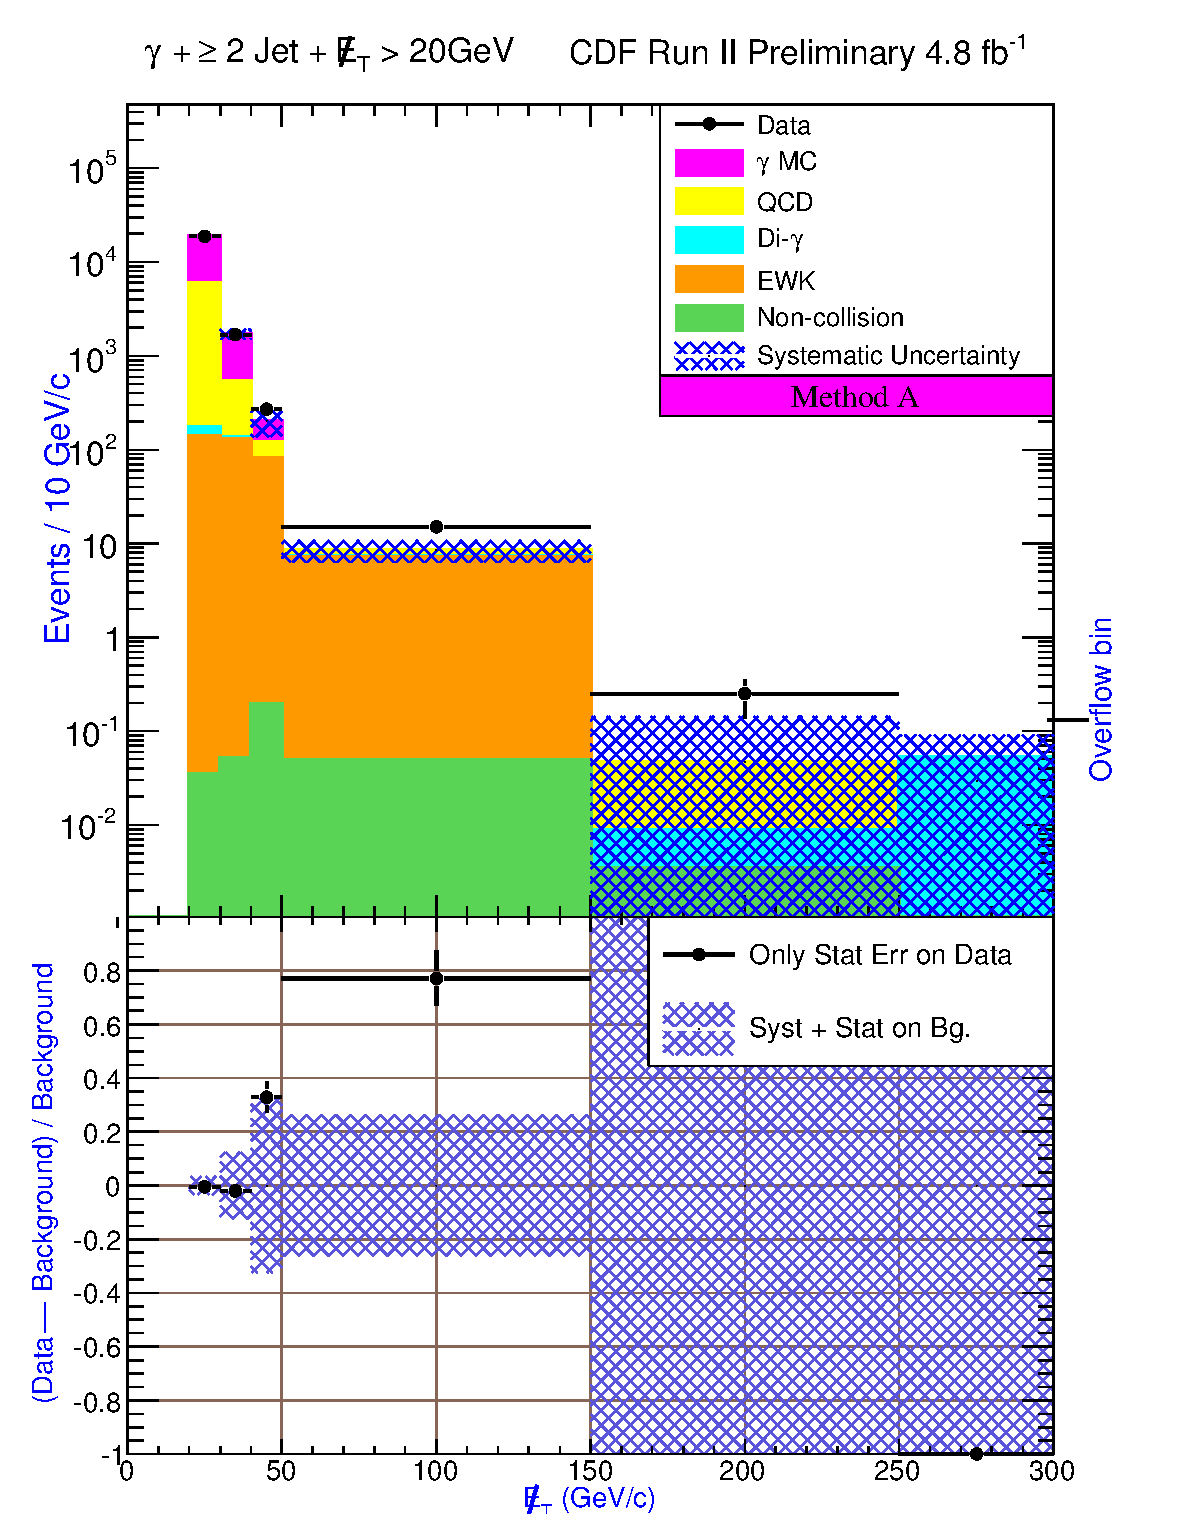
\includegraphics[keepaspectratio=true, scale=\figScale]{G30JetsMet20_MtdA_plot2_Met.pdf}}
\label{fig:pjMetSetFour}
\end{figure*}



\clearpage
%%%%%%%%%%%%%%%%%%%%%%%%%%%%%%%%%%%% METHOD B: G30 JETS

\begin{figure*}[h!]
 \centering
\caption[Method B \phoonejet]{Kinematic distributions of \phoonejet events using \mbox{Method B}. See Section~\ref{sec:PrelResults} for a description of the elements in these distributions.}
\subfigure[]
{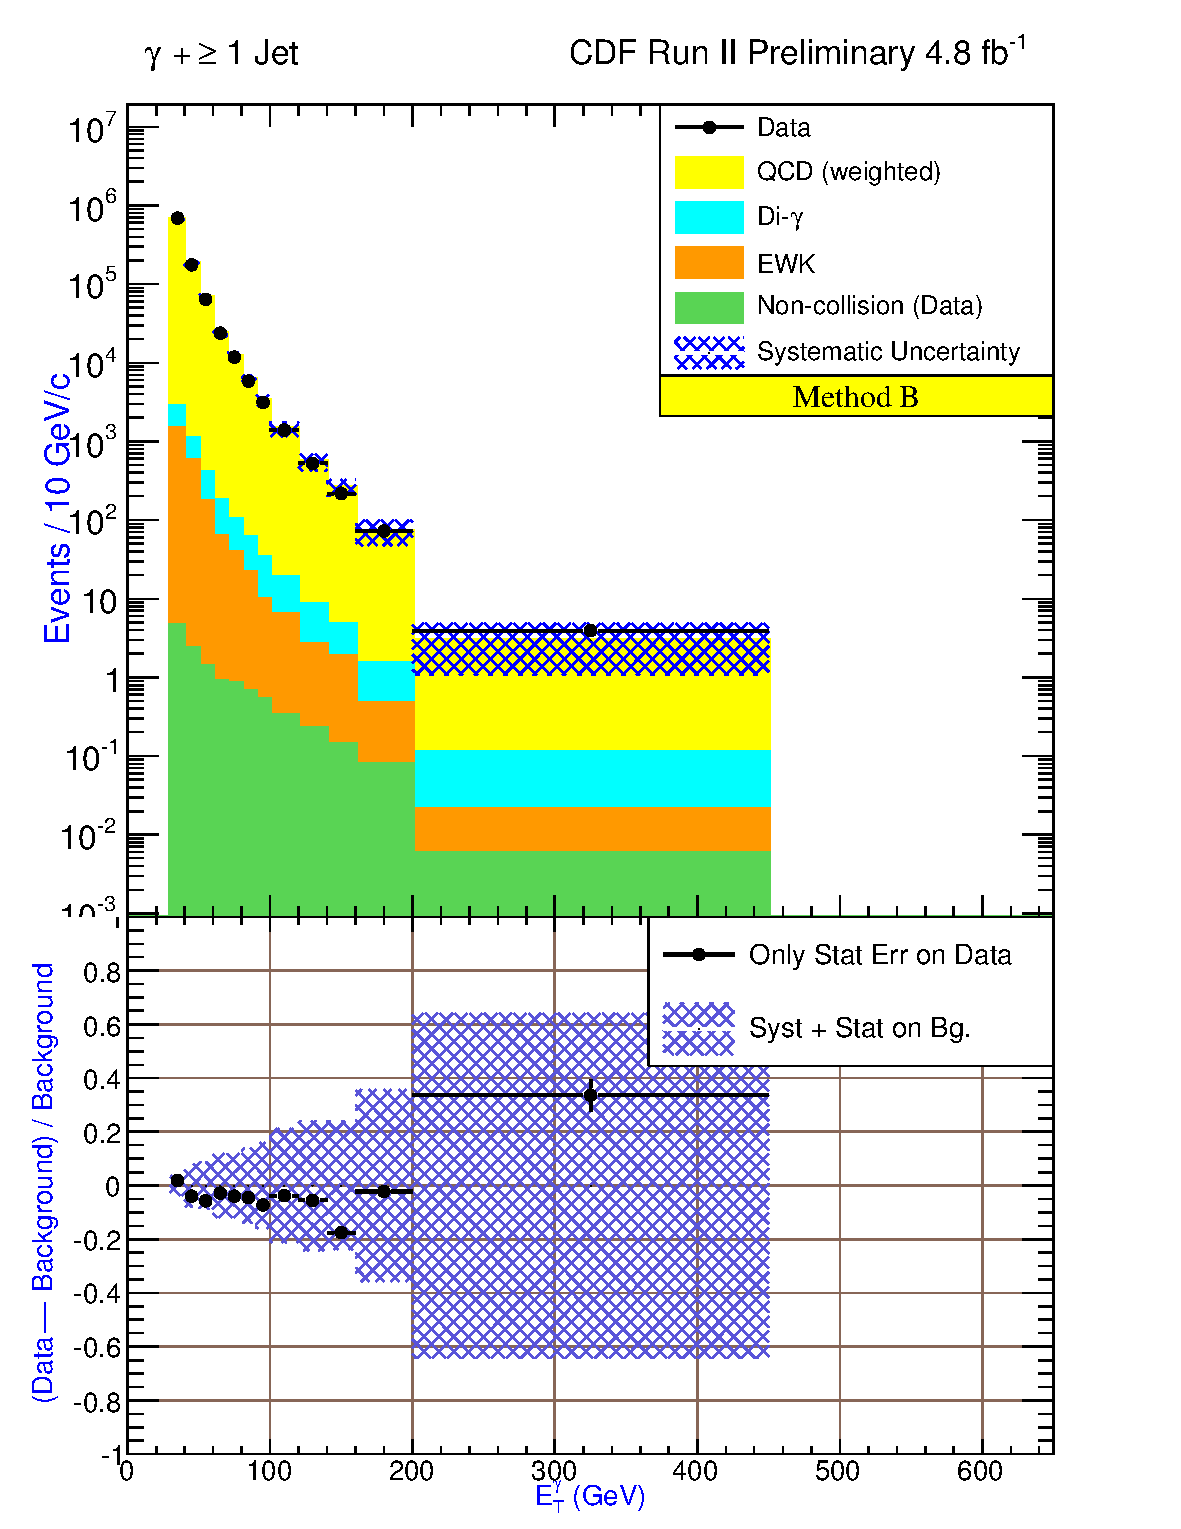
\includegraphics[keepaspectratio=true, scale=\figScale]{G30Jets_MtdB_plot1_Et_pho.pdf}}
\subfigure[]
{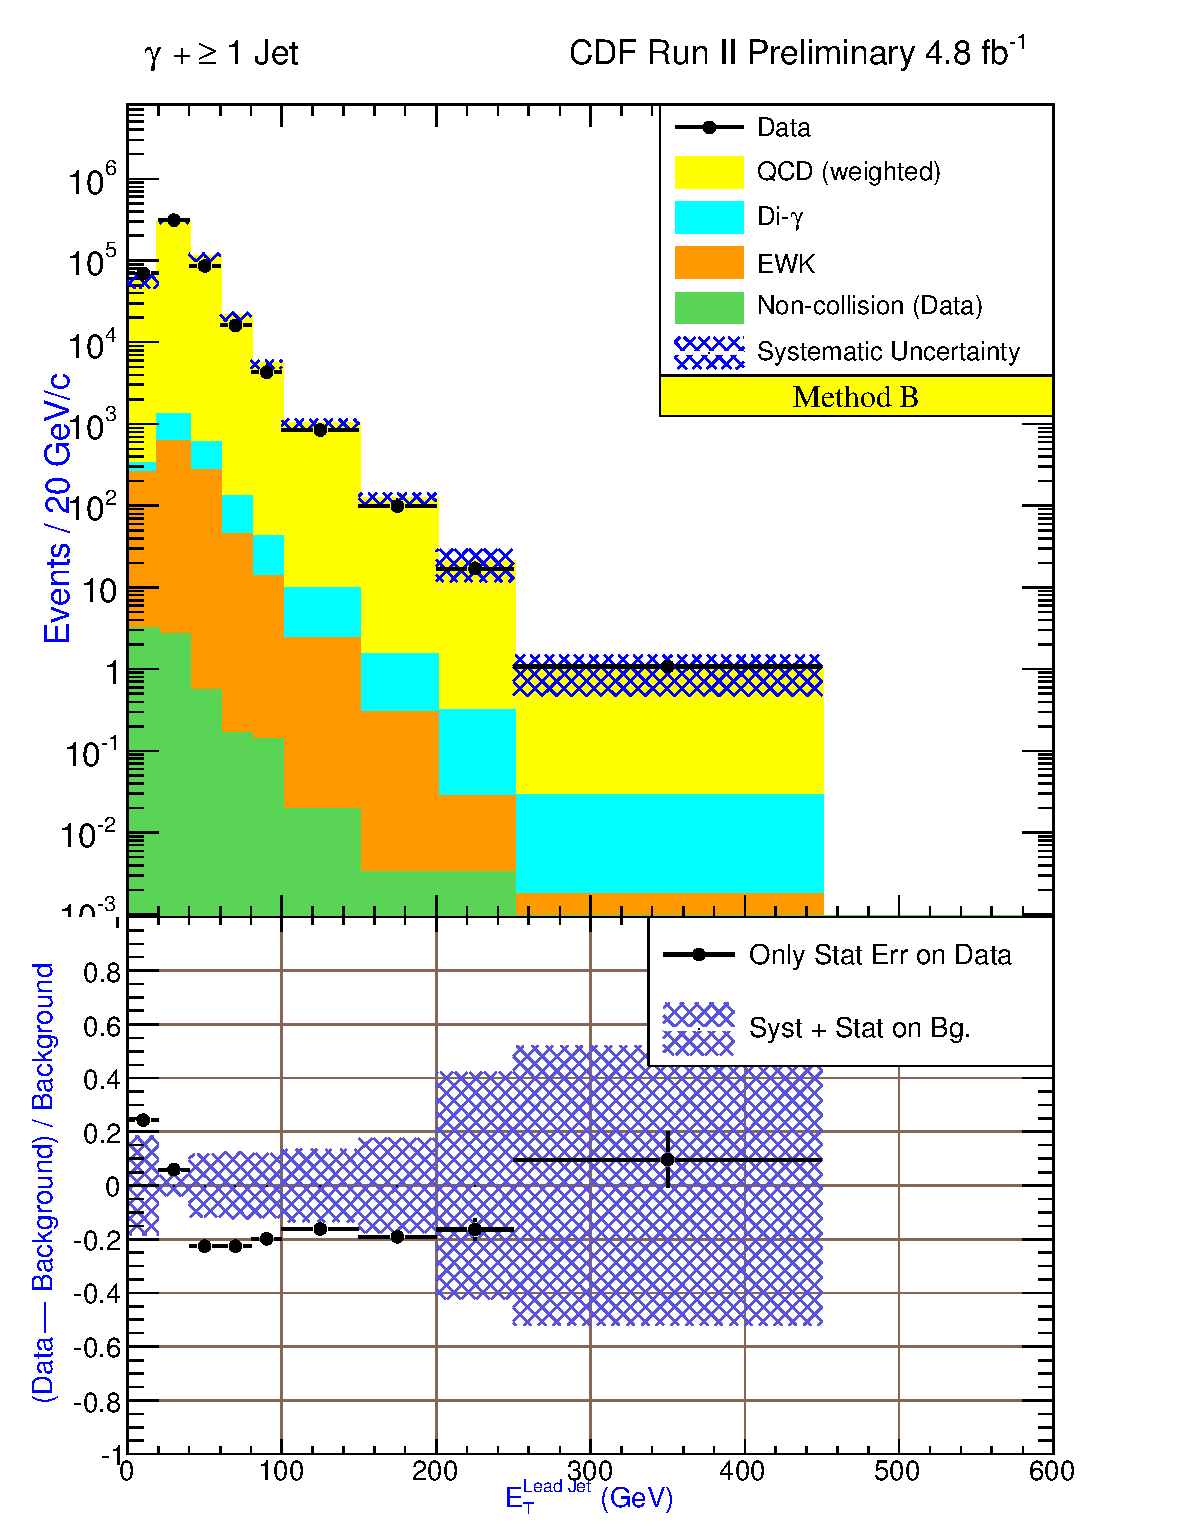
\includegraphics[keepaspectratio=true, scale=\figScale]{G30Jets_MtdB_plot1_Et_j1.pdf}}
\subfigure[]
{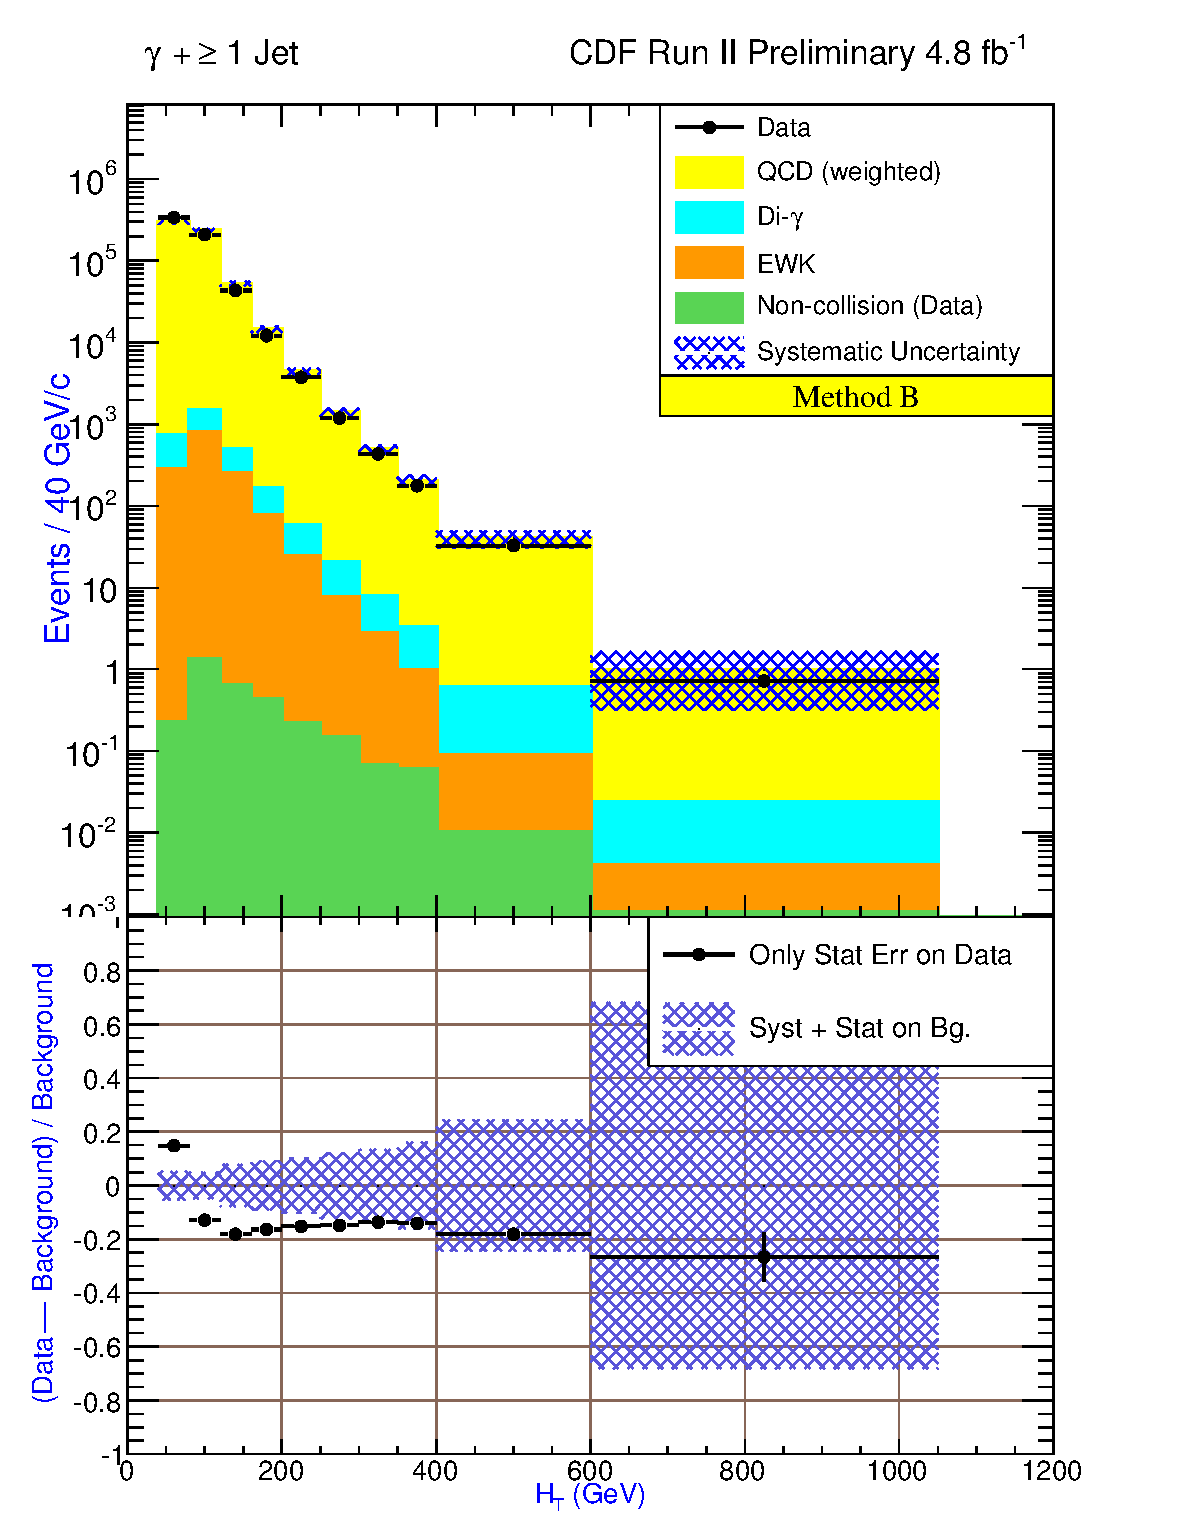
\includegraphics[keepaspectratio=true, scale=\figScale]{G30Jets_MtdB_plot1_Ht.pdf}}
\subfigure[]
{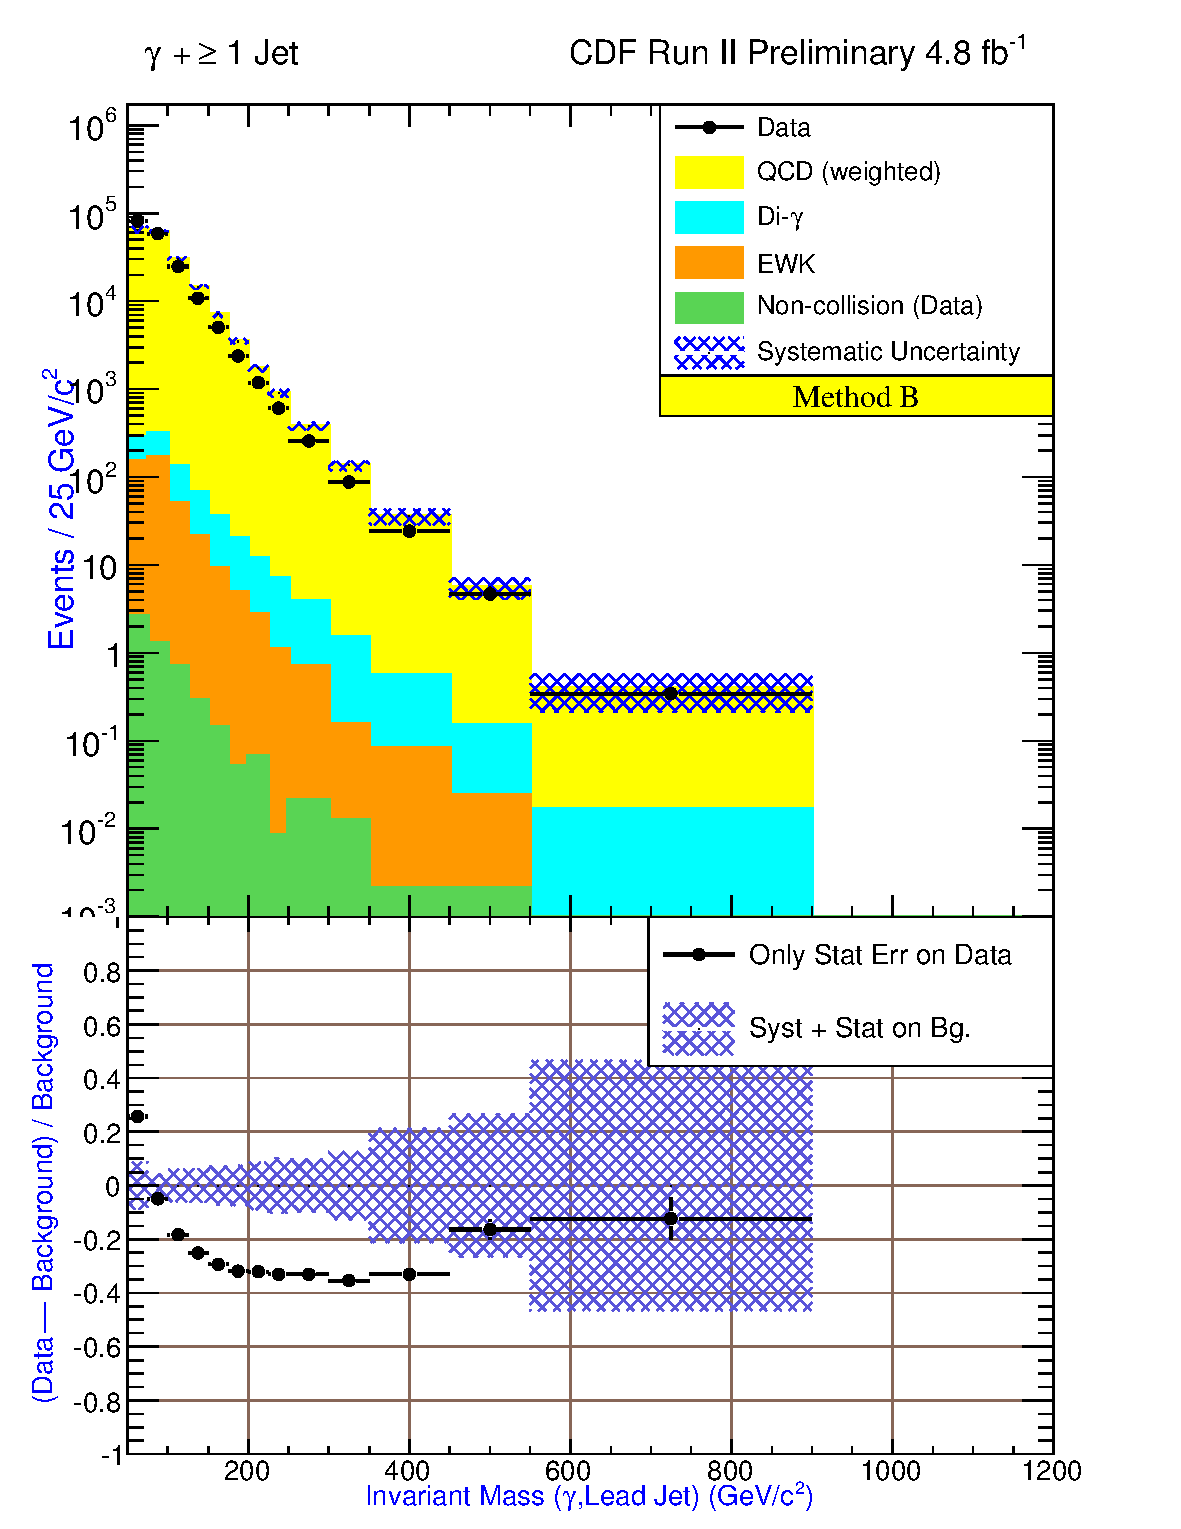
\includegraphics[keepaspectratio=true, scale=\figScale]{G30Jets_MtdB_plot1_InvMass_pj1.pdf}
\label{fig:pjMtdBSetOne:Mass_pj1}
}
\label{fig:pjMtdBSetOne}
\end{figure*}
\clearpage

\begin{figure*}[h!]
\centering
\caption[Method B \phoonejet]{Kinematic distributions of \phoonejet and \photwojet events using \mbox{Method B}. See Section~\ref{sec:PrelResults} for a description of the elements in these distributions.}
\subfigure[]
{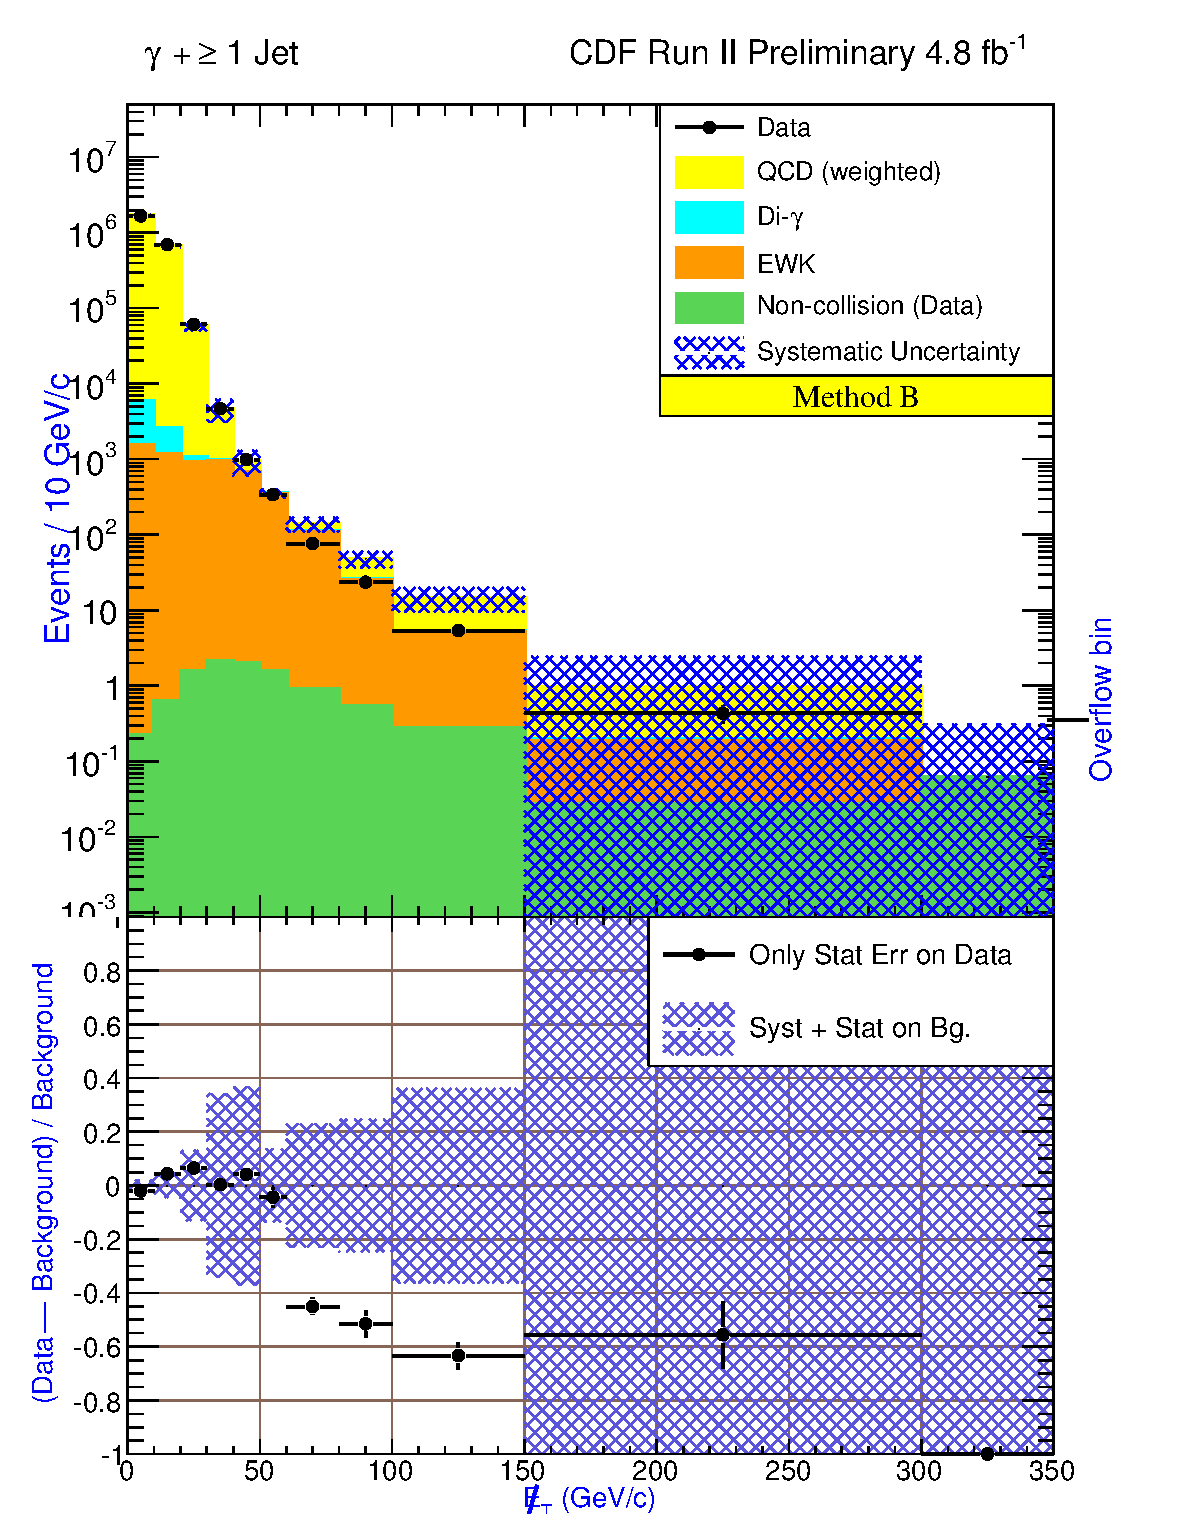
\includegraphics[keepaspectratio=true, scale=\figScale]{G30Jets_MtdB_plot1_Met.pdf}}
\subfigure[]
{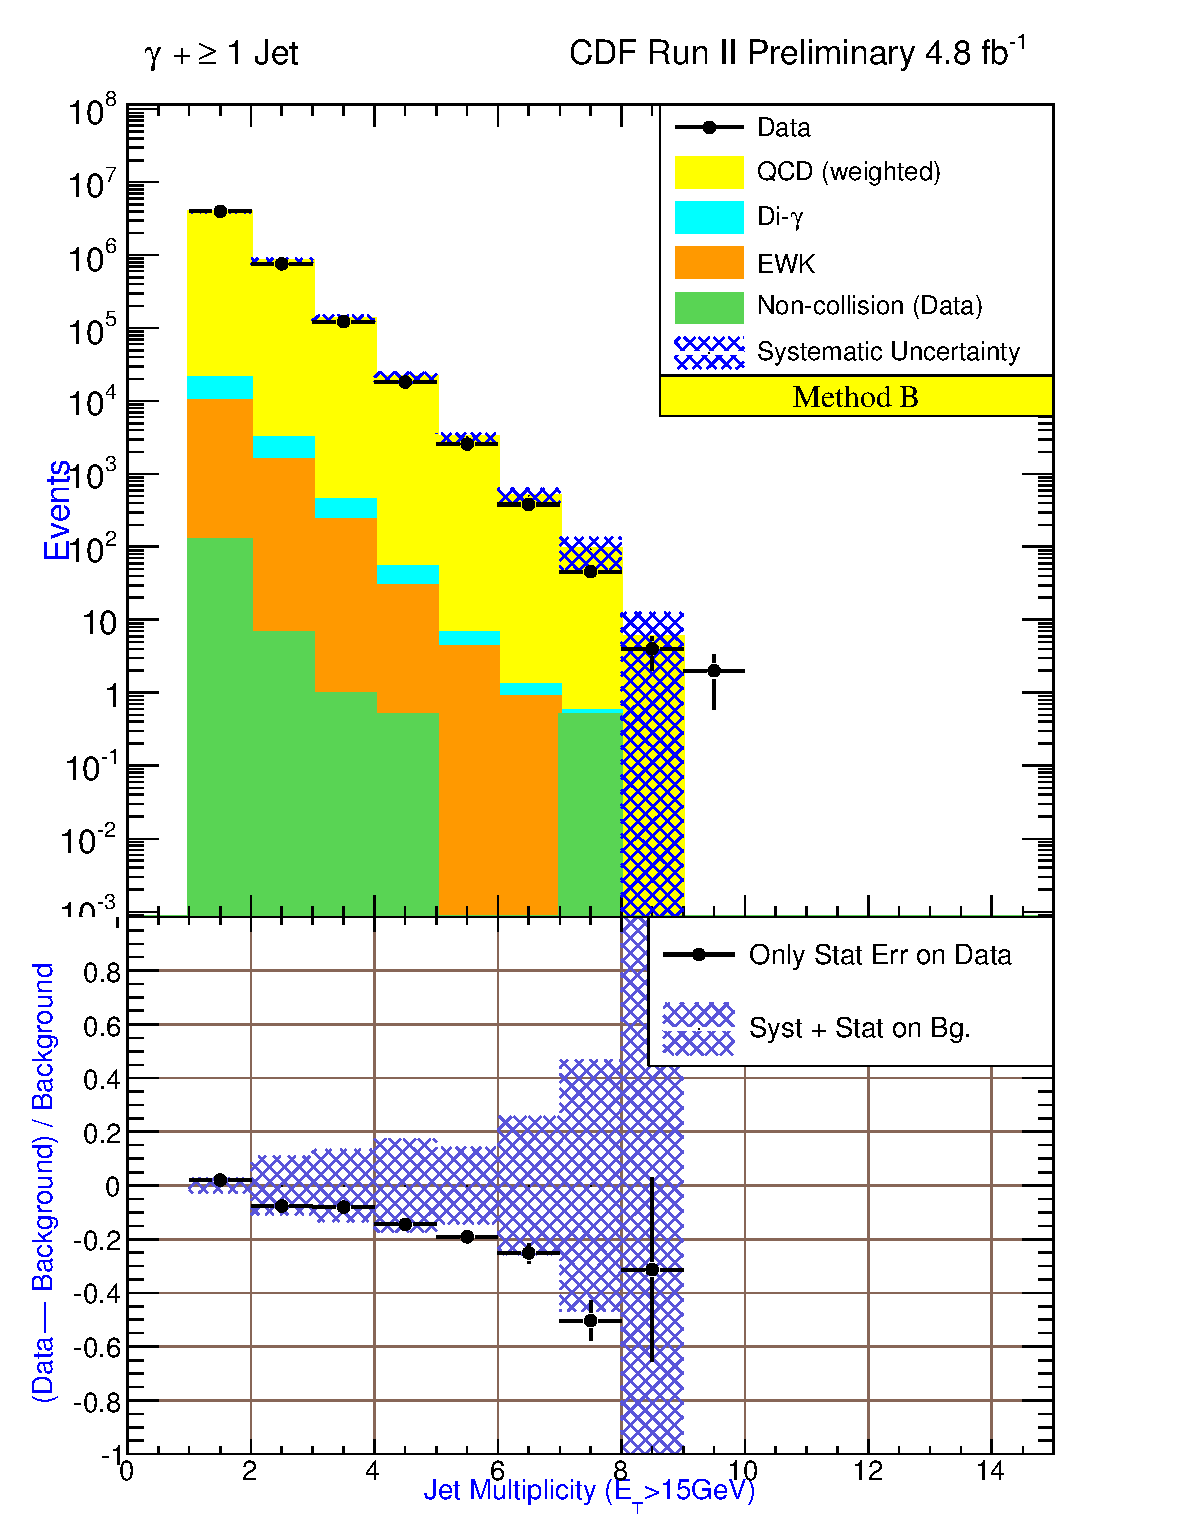
\includegraphics[keepaspectratio=true, scale=\figScale]{G30Jets_MtdB_plot1_NJet.pdf}}
\subfigure[]
{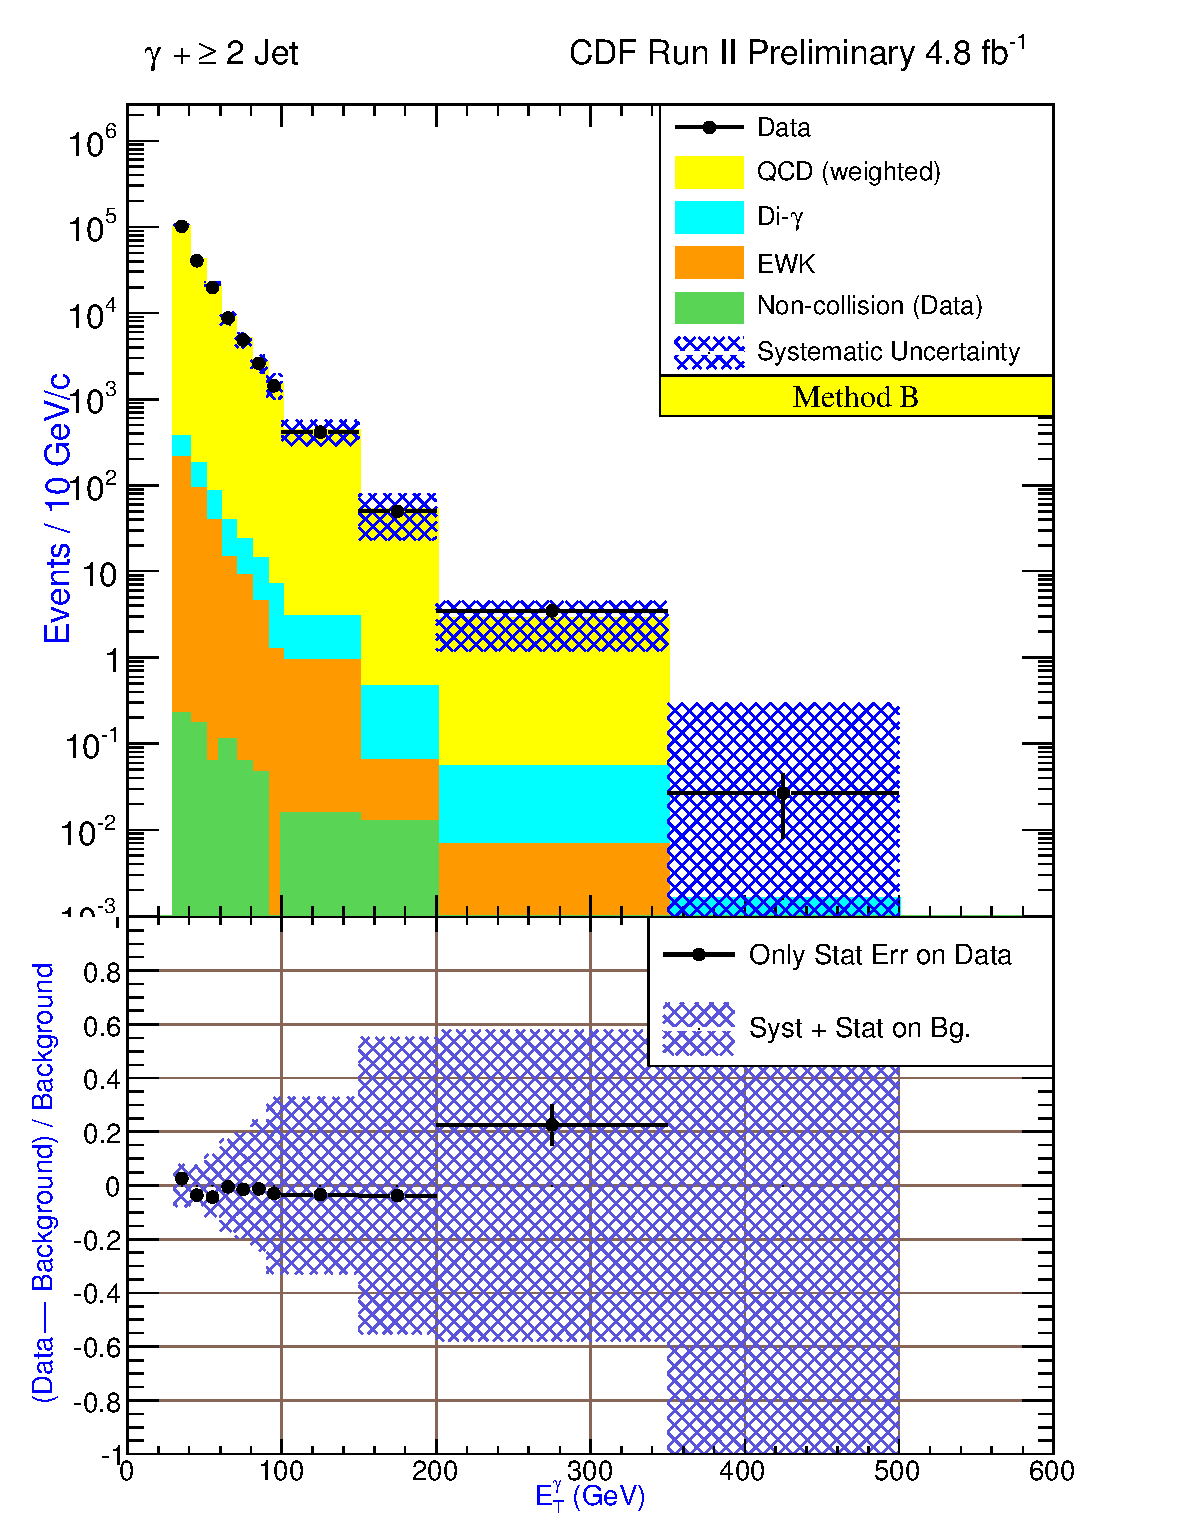
\includegraphics[keepaspectratio=true, scale=\figScale]{G30Jets_MtdB_plot2_Et_pho.pdf}}
\subfigure[]
{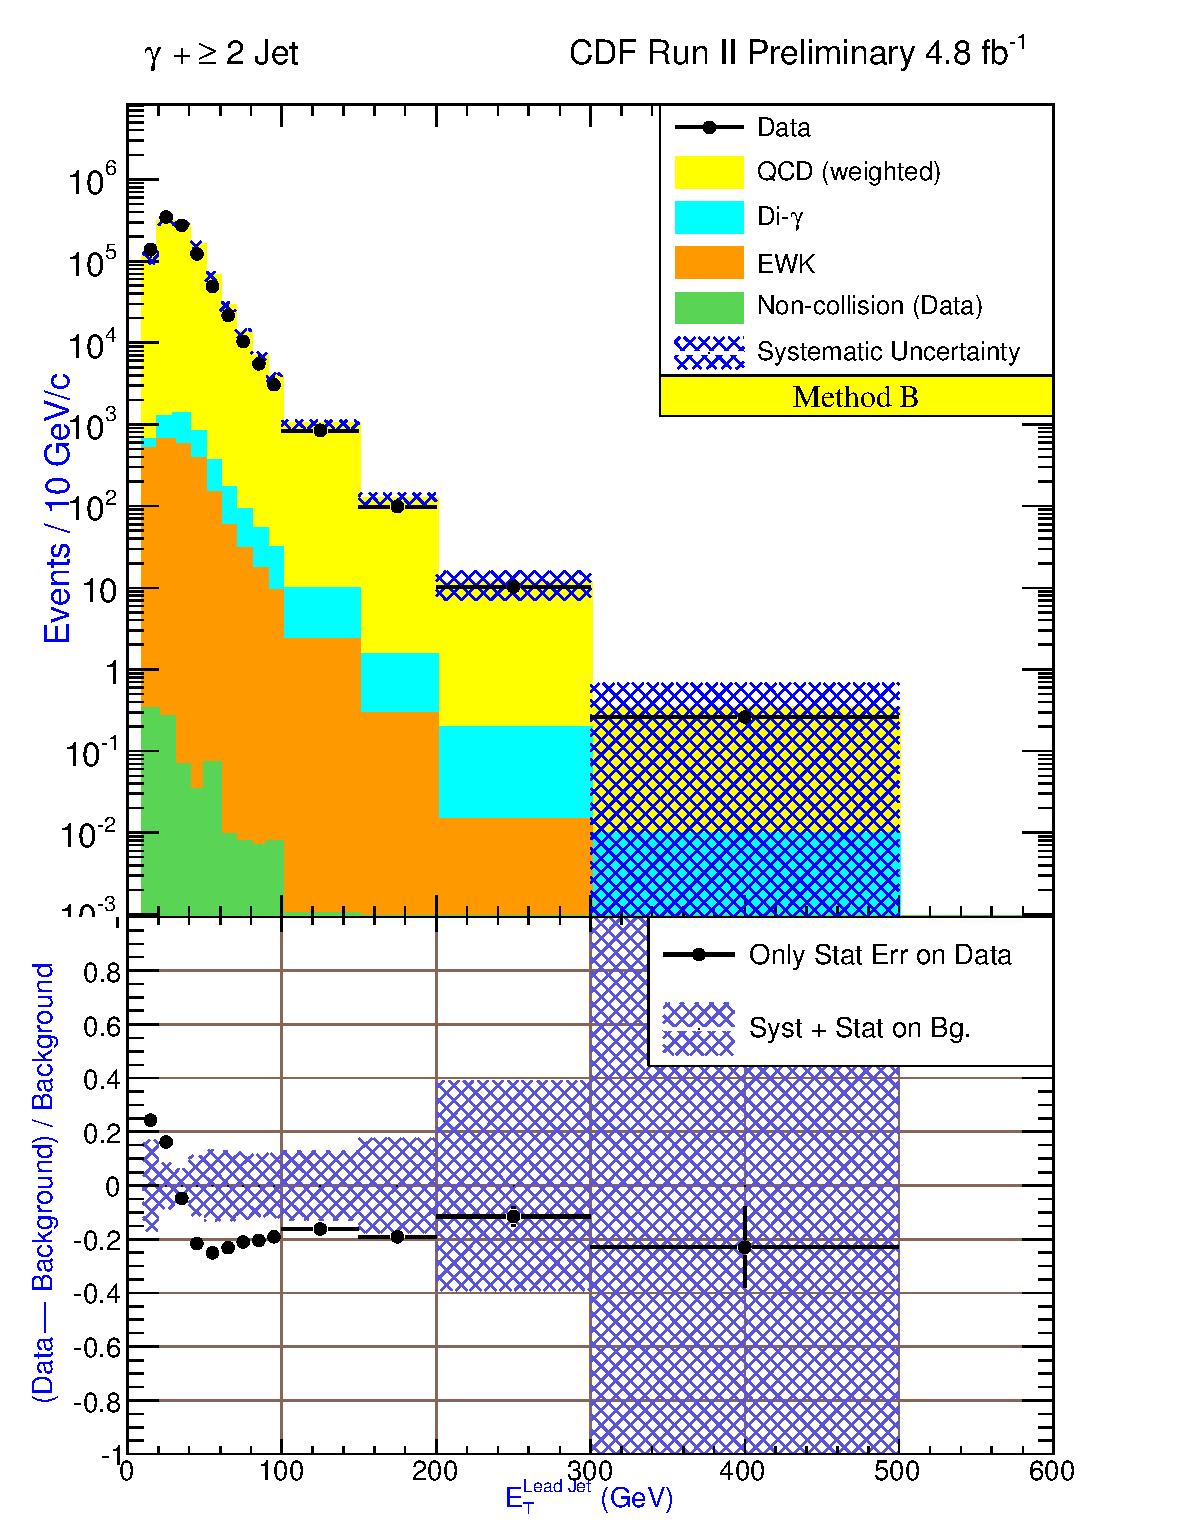
\includegraphics[keepaspectratio=true, scale=\figScale]{G30Jets_MtdB_plot2_Et_j1.pdf}}
\label{fig:pjMtdBSetTwo}
\end{figure*}
\clearpage

\begin{figure*}[h!]
\centering
\caption[Method B \photwojet]{Kinematic distributions of \photwojet events using \mbox{Method B}. See Section~\ref{sec:PrelResults} for a description of the elements in these distributions.}
\subfigure[]
{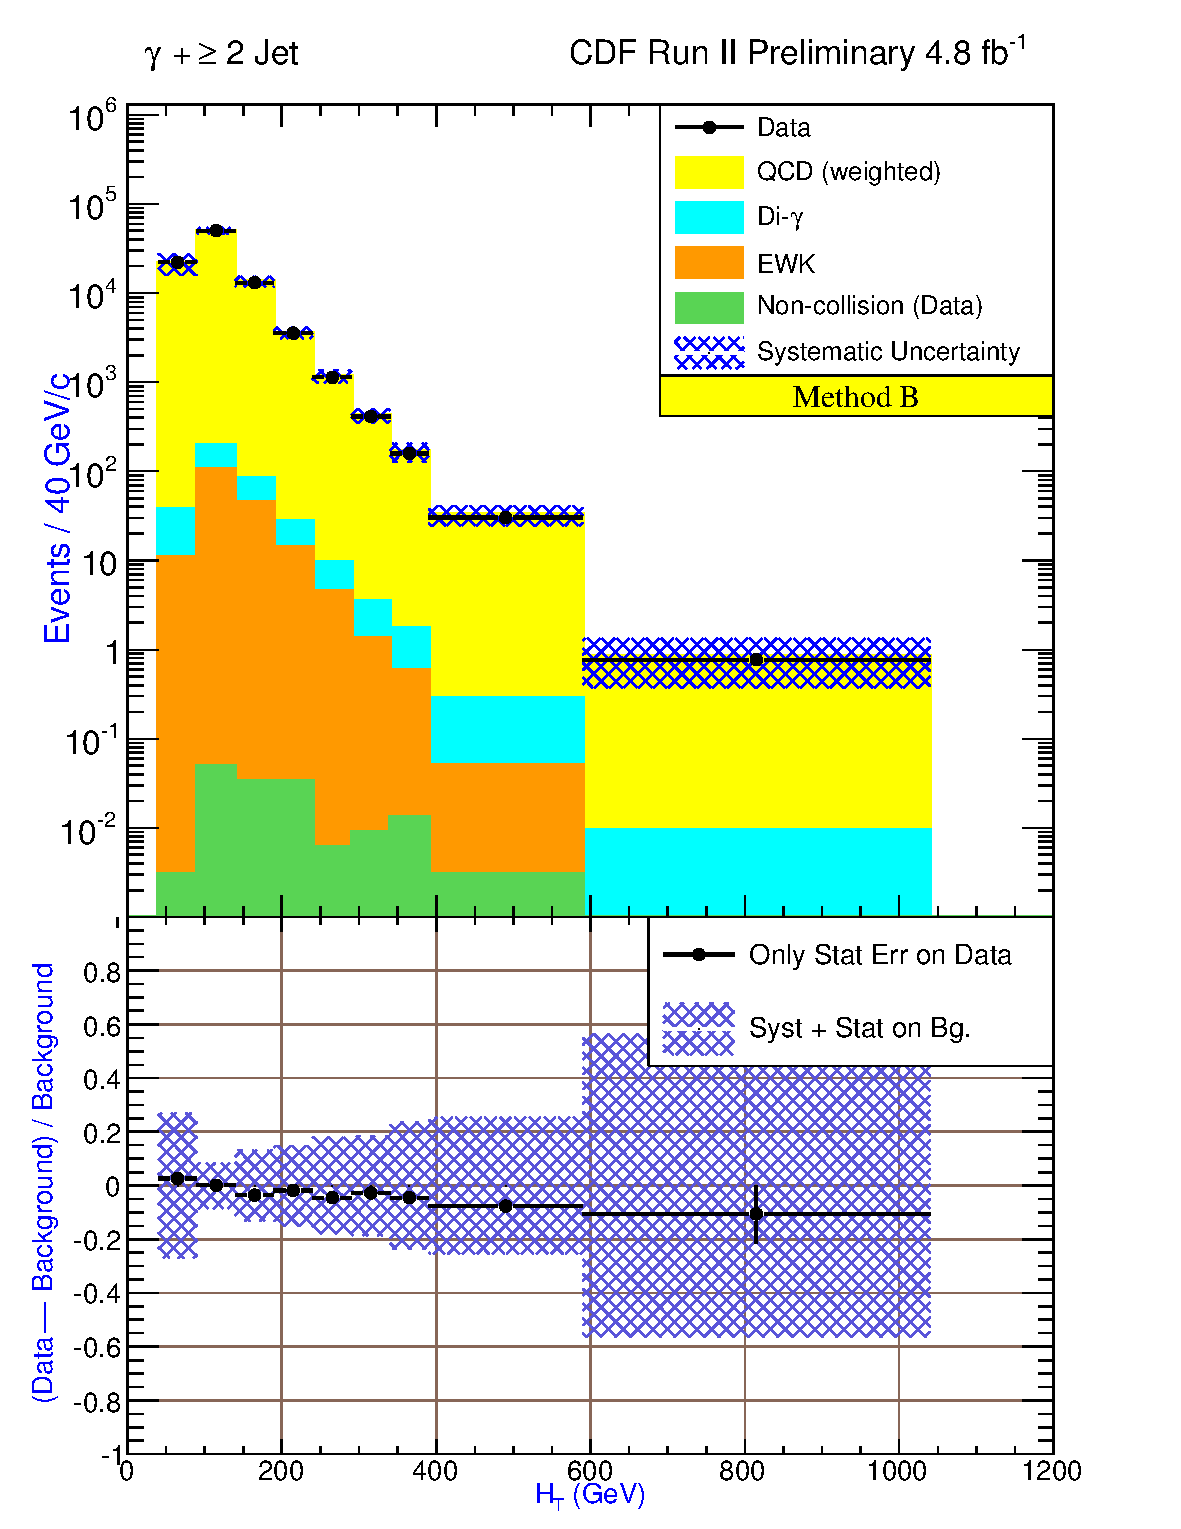
\includegraphics[keepaspectratio=true, scale=\figScale]{G30Jets_MtdB_plot2_Ht.pdf}}
\subfigure[]
{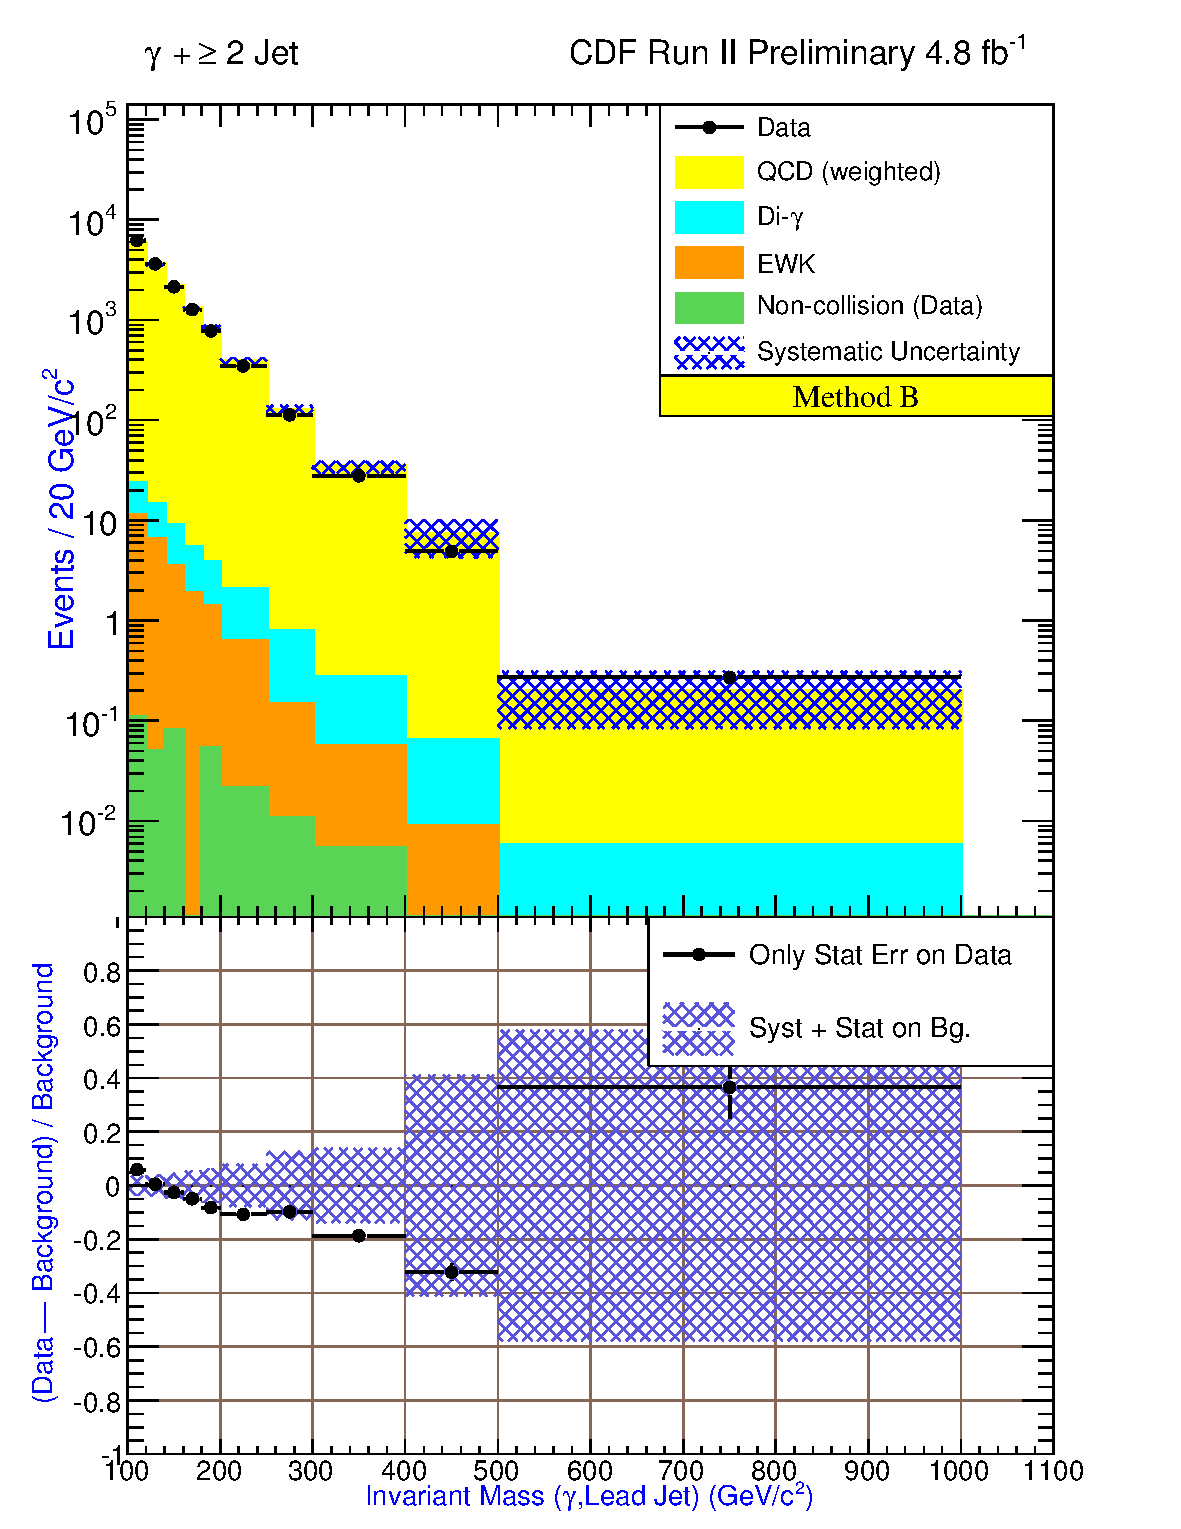
\includegraphics[keepaspectratio=true, scale=\figScale]{G30Jets_MtdB_plot2_InvMass_pj1.pdf}}
\subfigure[]
{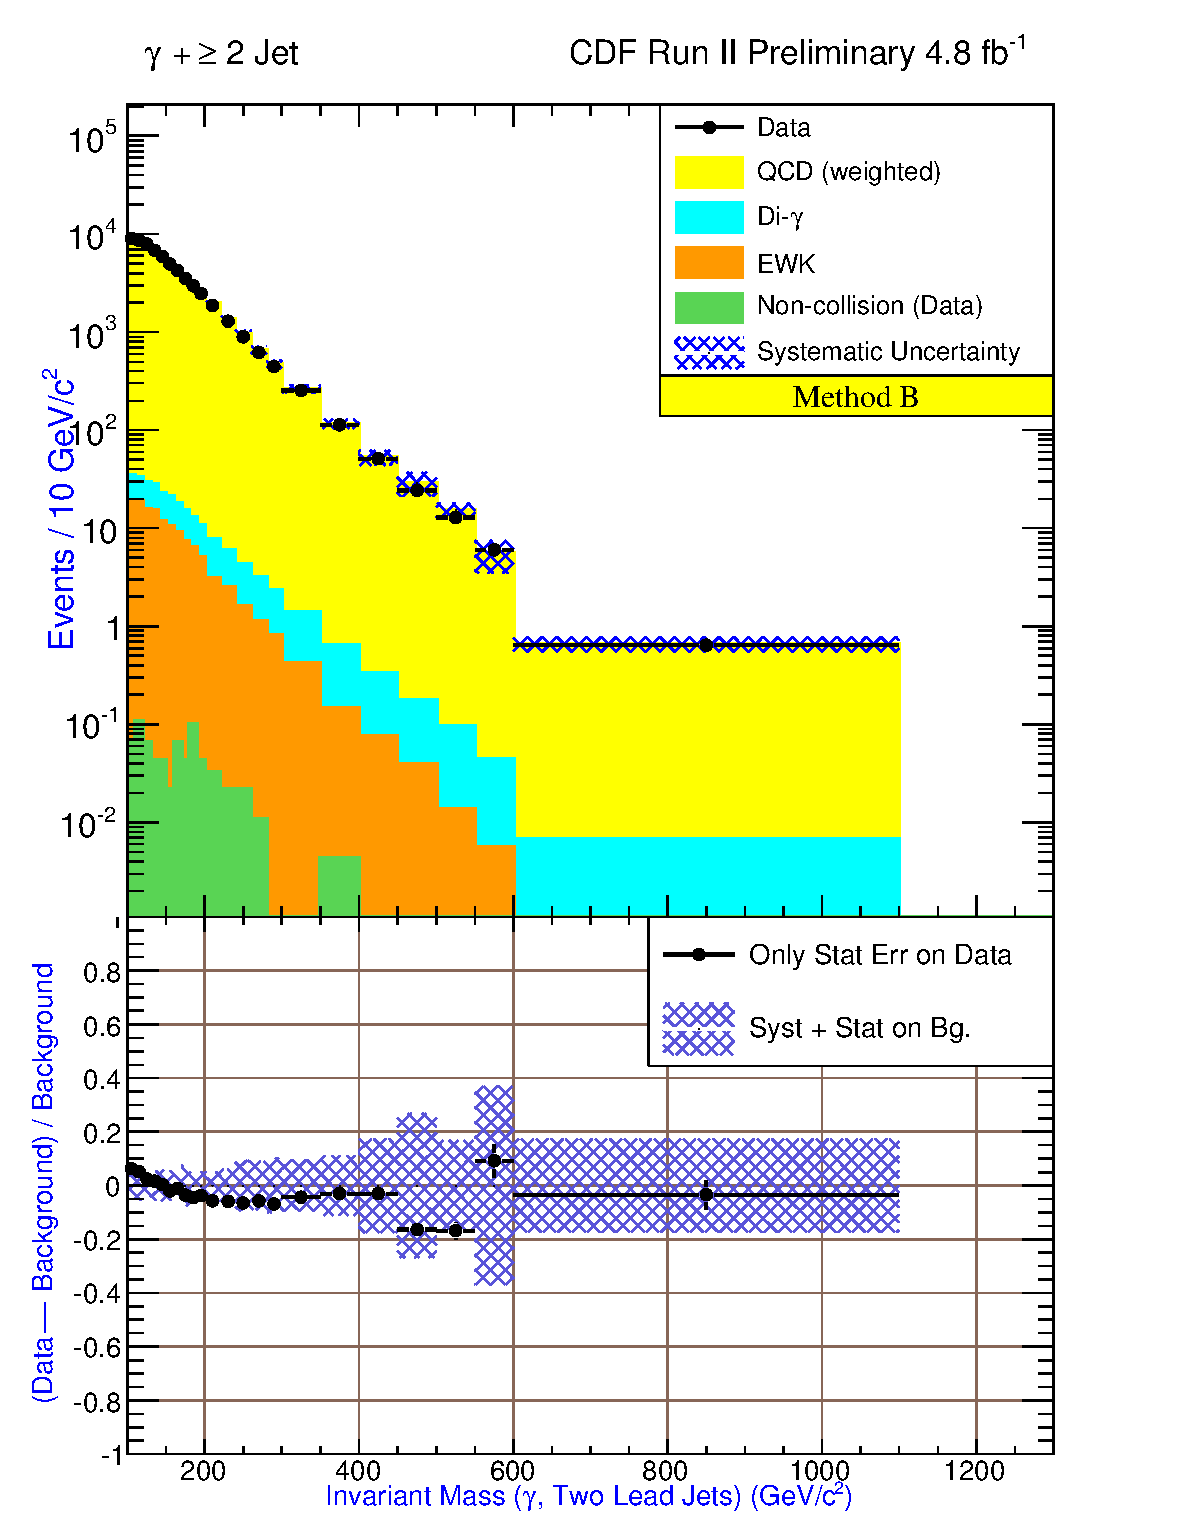
\includegraphics[keepaspectratio=true, scale=\figScale]{G30Jets_MtdB_plot2_InvMass_pj1j2.pdf}}
\subfigure[]
{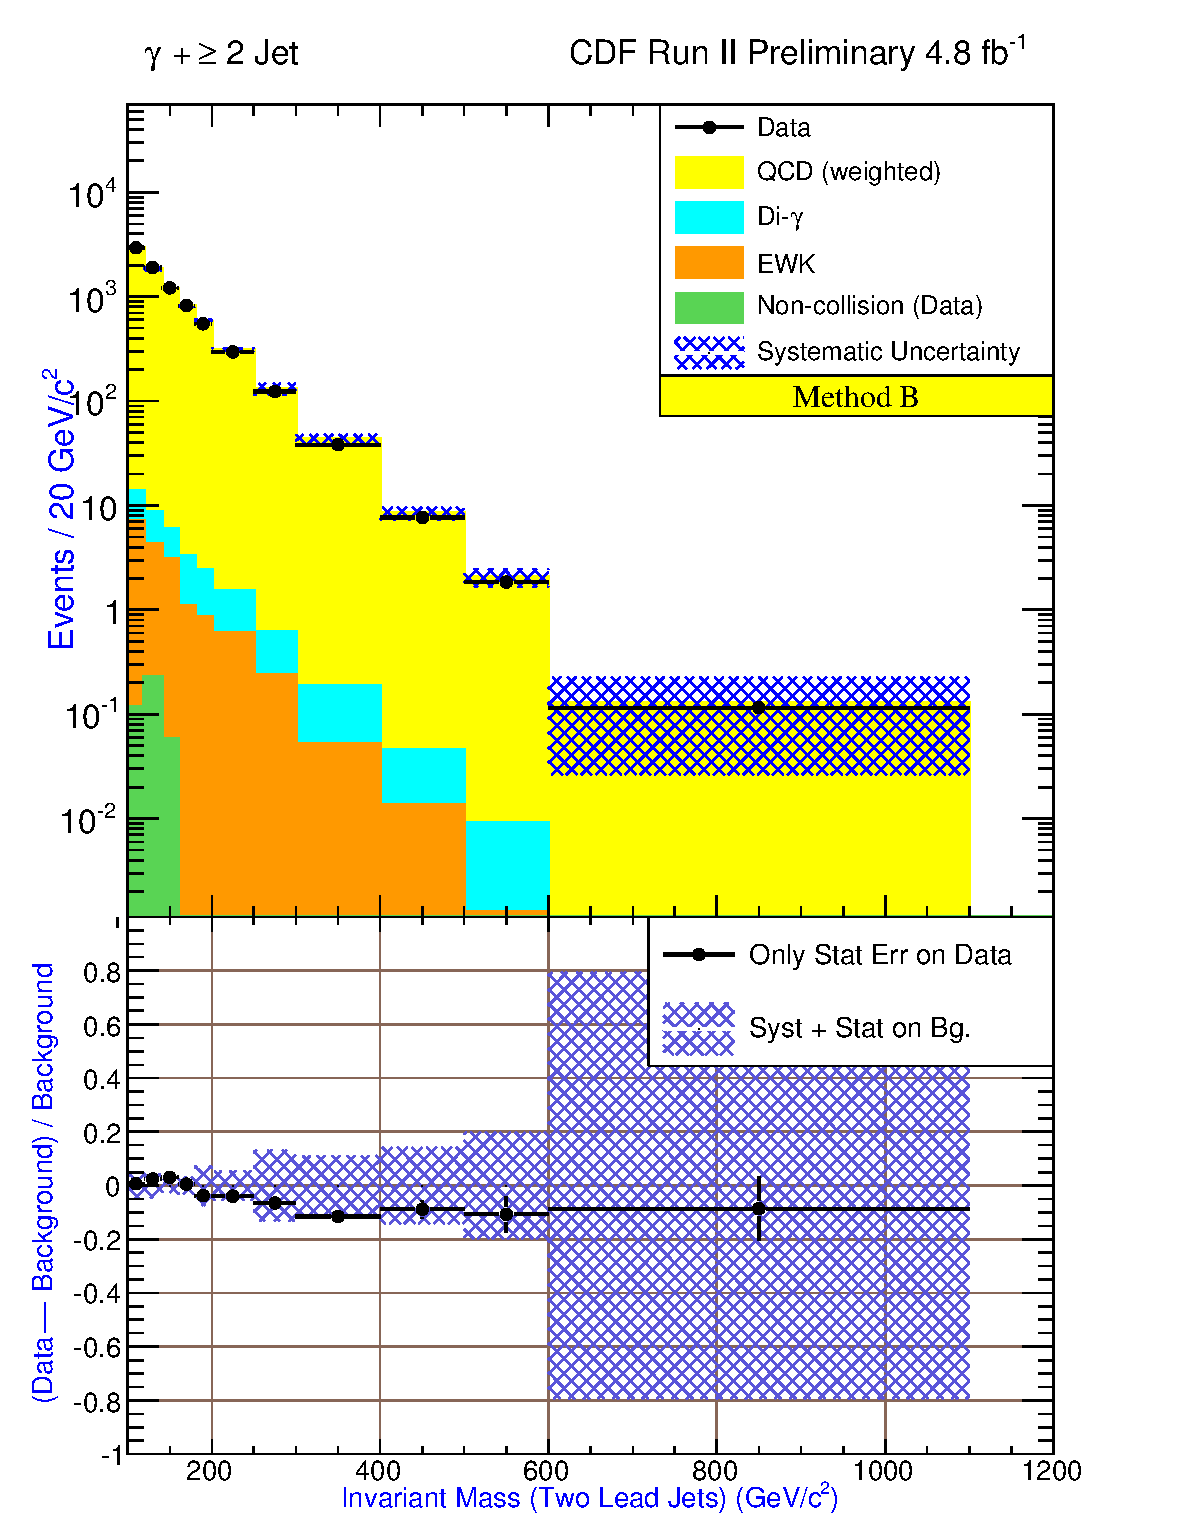
\includegraphics[keepaspectratio=true, scale=\figScale]{G30Jets_MtdB_plot2_InvMass_j1j2.pdf}}
\label{fig:pjMtdBSetThree}
\end{figure*}
\clearpage

\begin{figure*}[h!]
\centering
\caption[Method B \photwojet]{Kinematic distributions of \photwojet events using \mbox{Method B}. See Section~\ref{sec:PrelResults} for a description of the elements in these distributions.}
{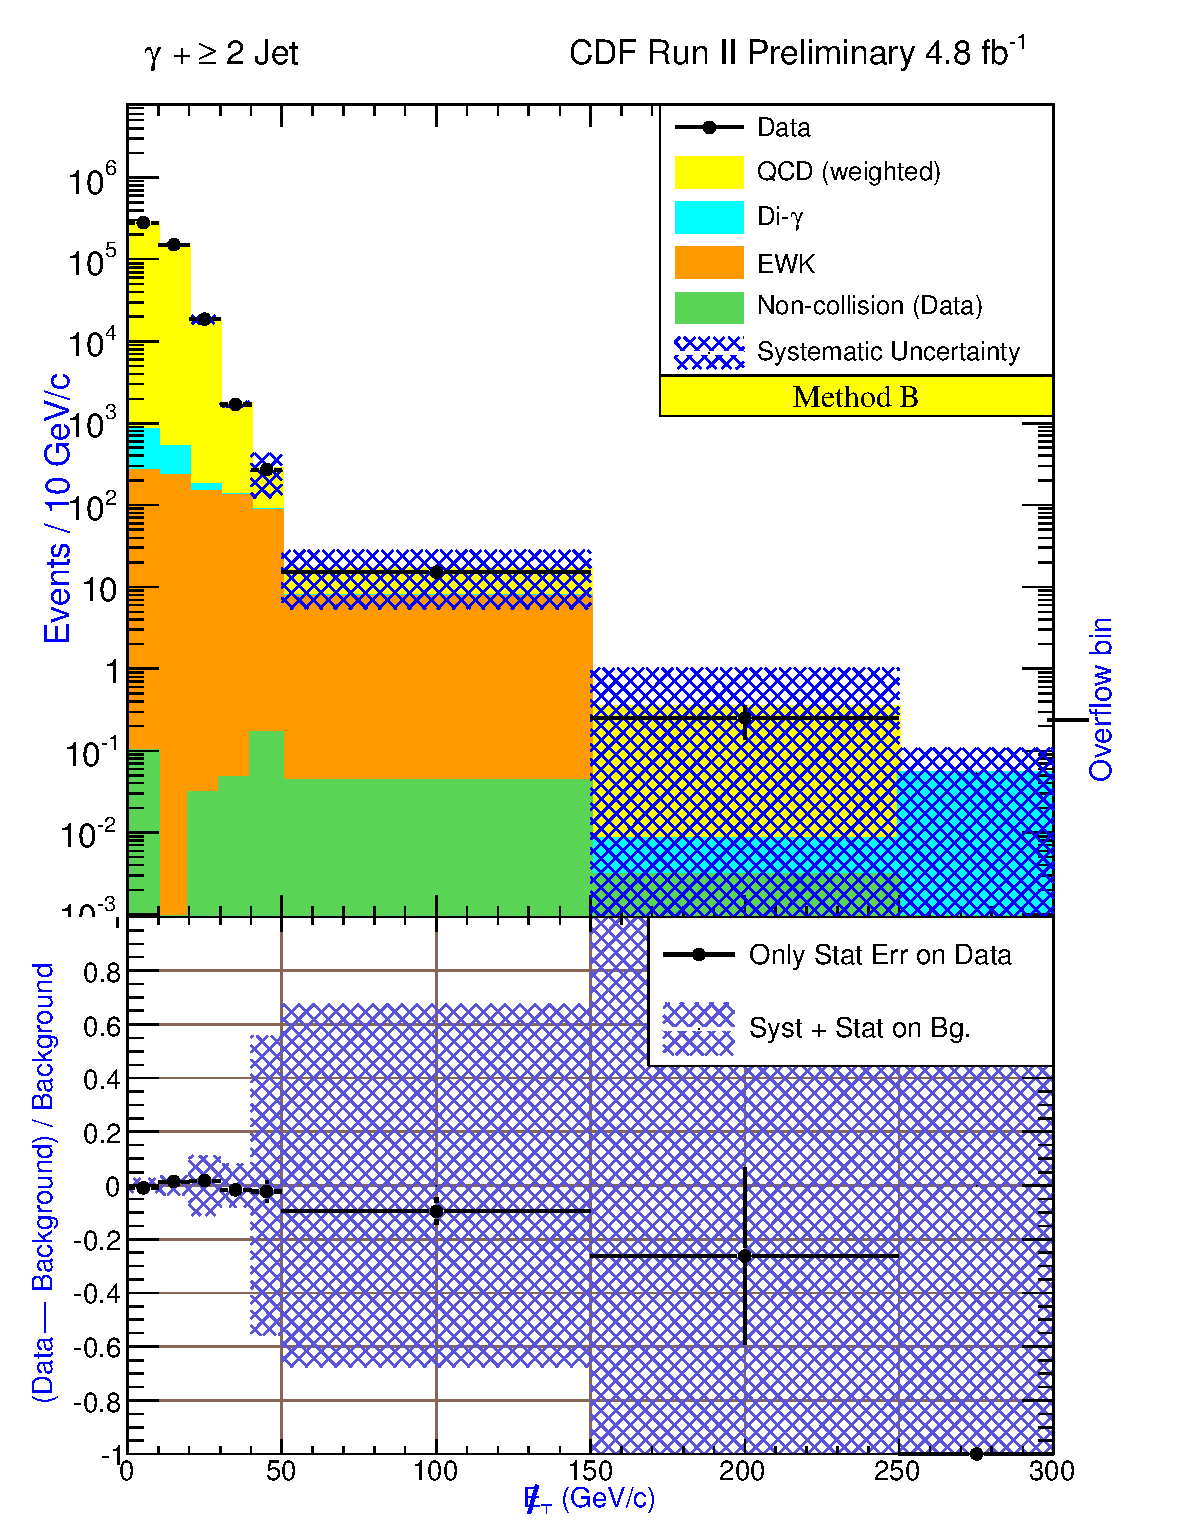
\includegraphics[keepaspectratio=true, scale=\figScale]{G30Jets_MtdB_plot2_Met.pdf}}
\label{fig:pjMtdBSetFour}
\end{figure*}
\clearpage

%%%%%%%%%%%%%%%%%%%%%%%%%%%%%%%%%%%% METHOD B: G30 JETS+MET>20

\begin{figure*}[h!]
 \centering
\caption[Method B \phoonejet]{Kinematic distributions of \phoonejet + \met$>$~20~GeV events using \mbox{Method B}. See Section~\ref{sec:PrelResults} for a description of the elements in these distributions.}
{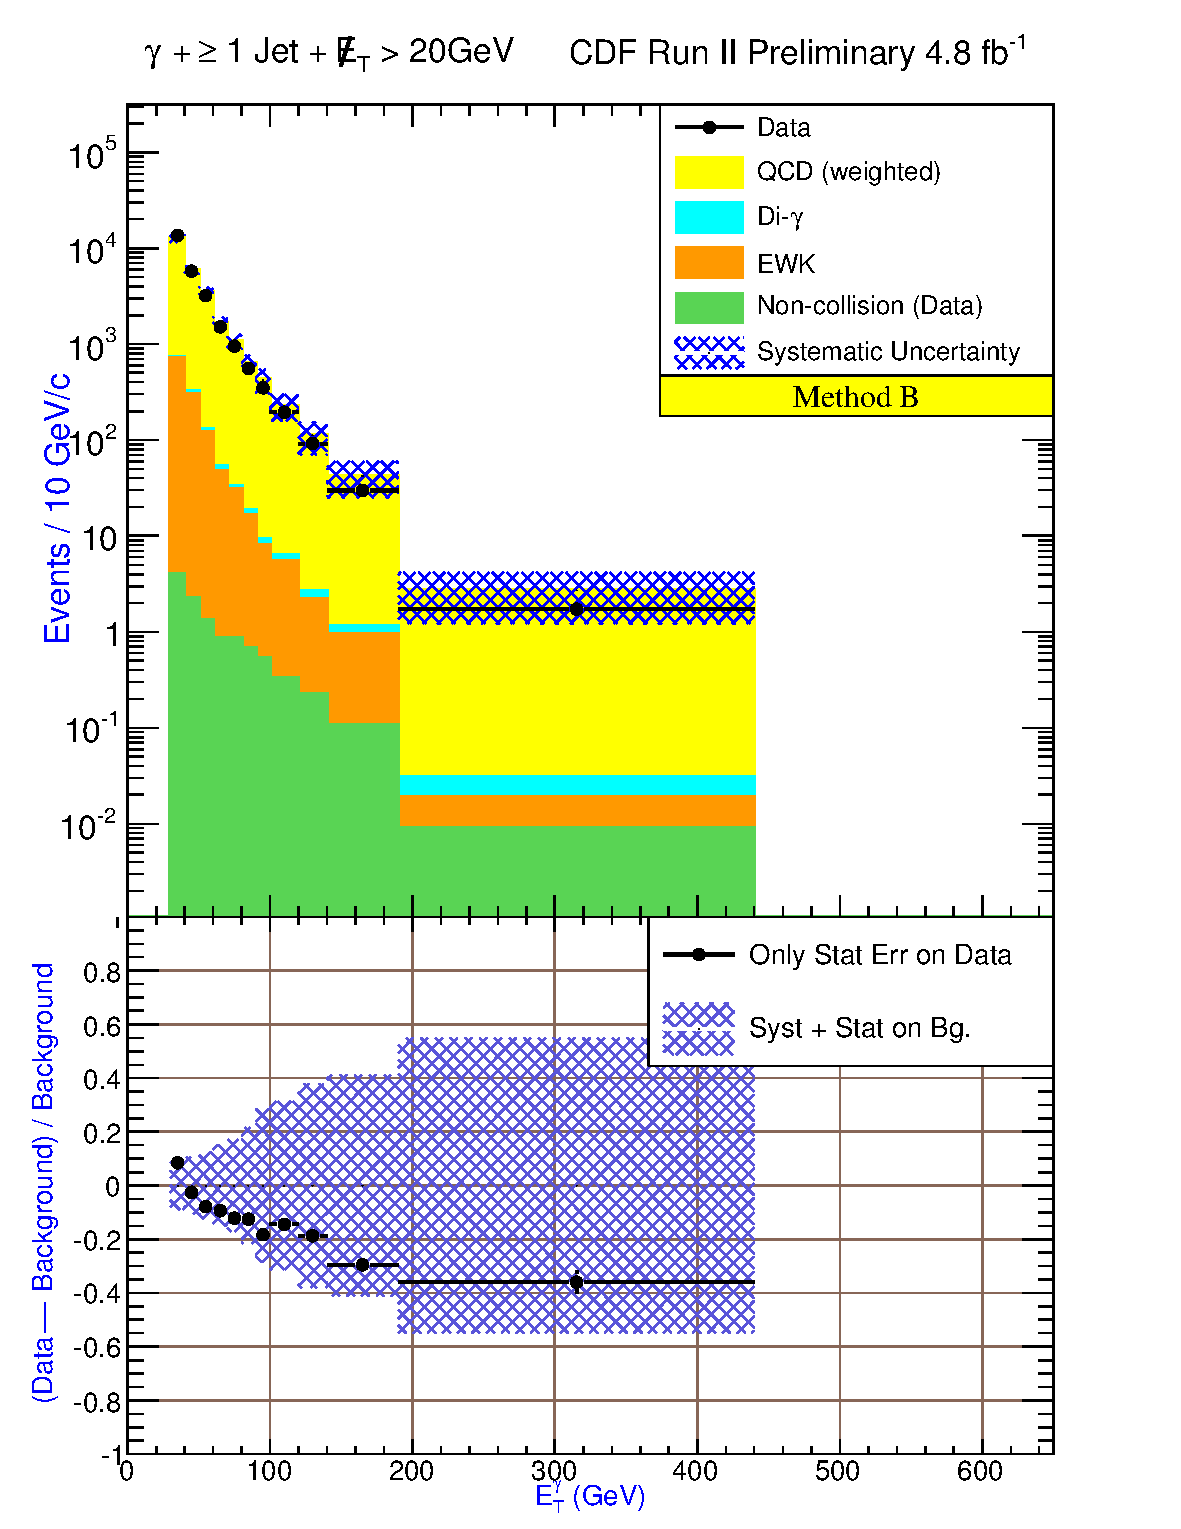
\includegraphics[keepaspectratio=true, scale=\figScale]{G30JetsMet20_MtdB_plot1_Et_pho.pdf}}
{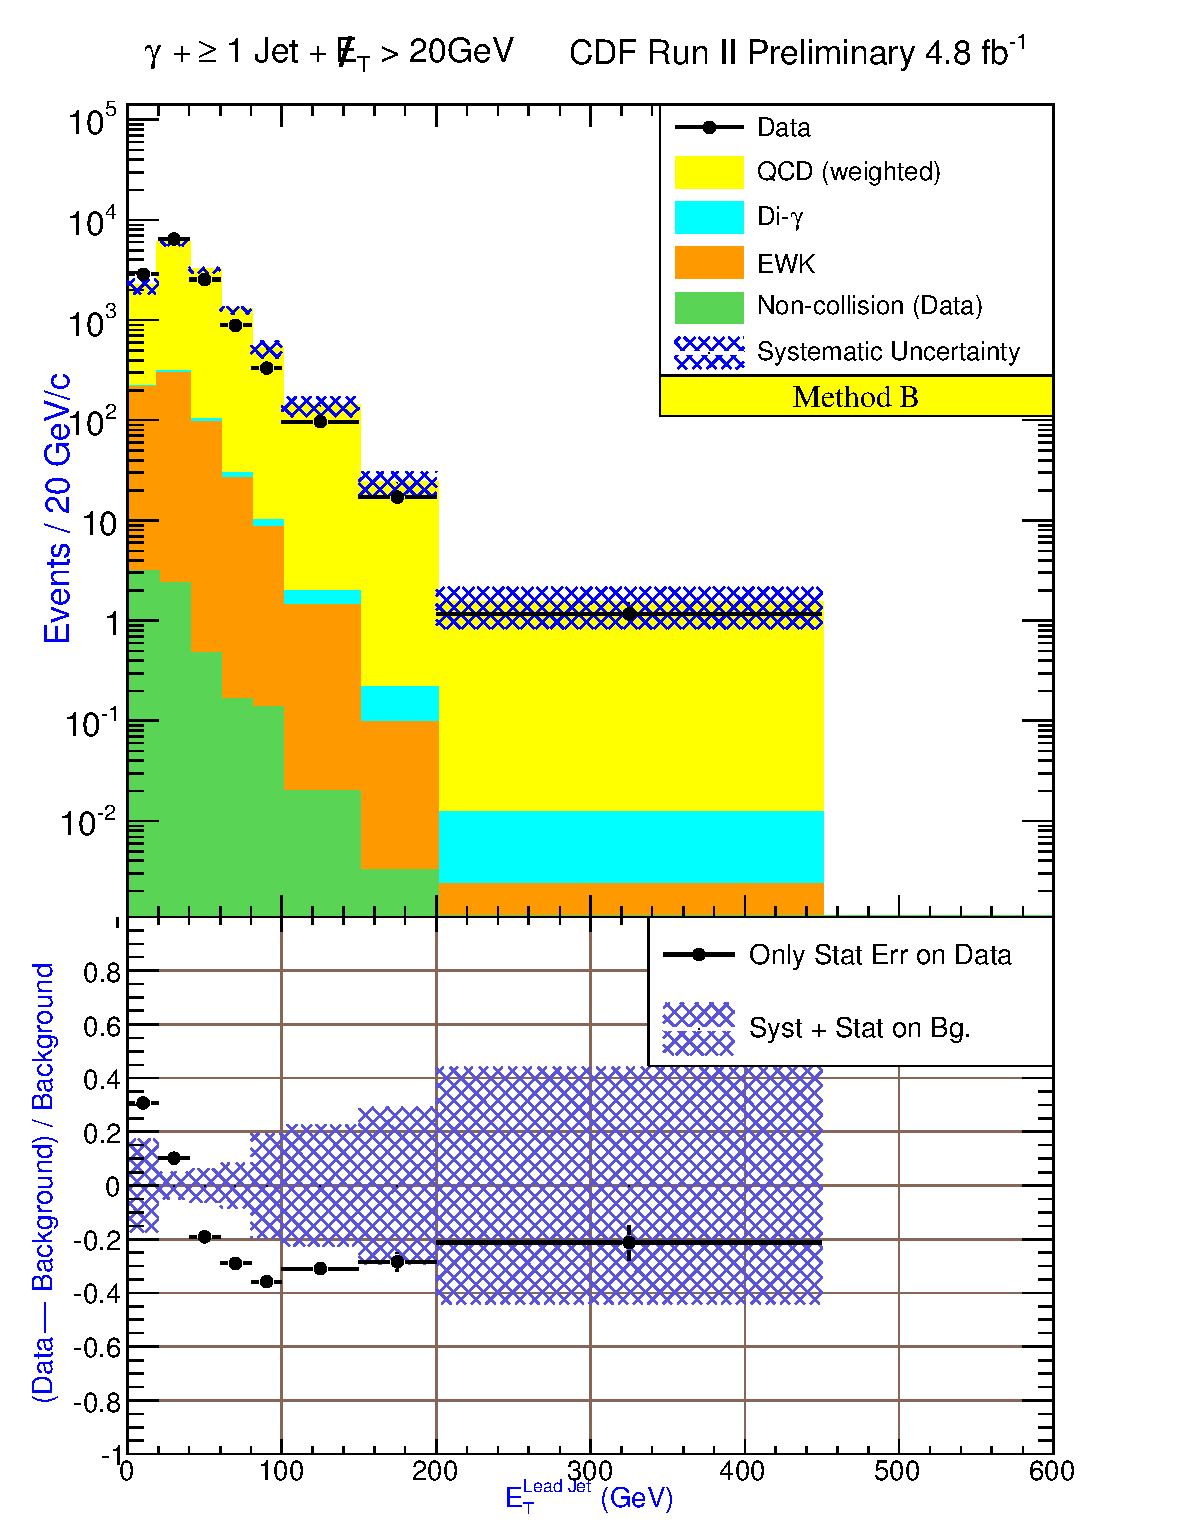
\includegraphics[keepaspectratio=true, scale=\figScale]{G30JetsMet20_MtdB_plot1_Et_j1.pdf}}
{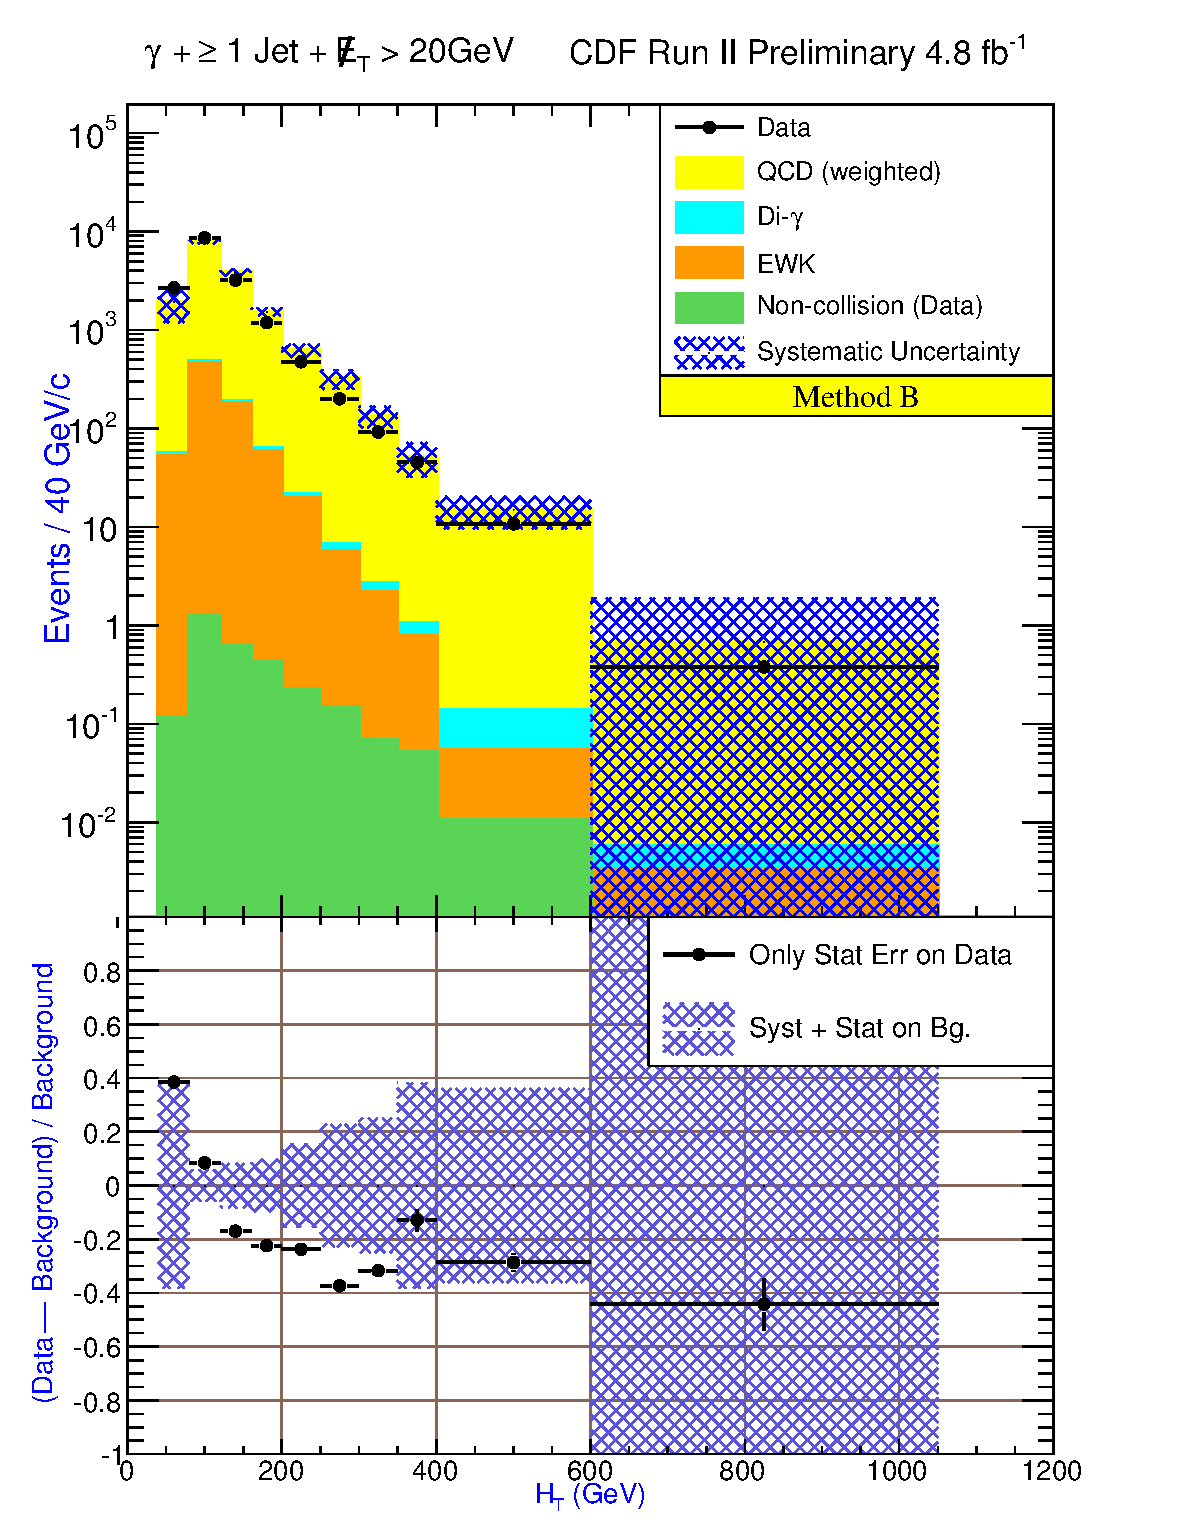
\includegraphics[keepaspectratio=true, scale=\figScale]{G30JetsMet20_MtdB_plot1_Ht.pdf}}
{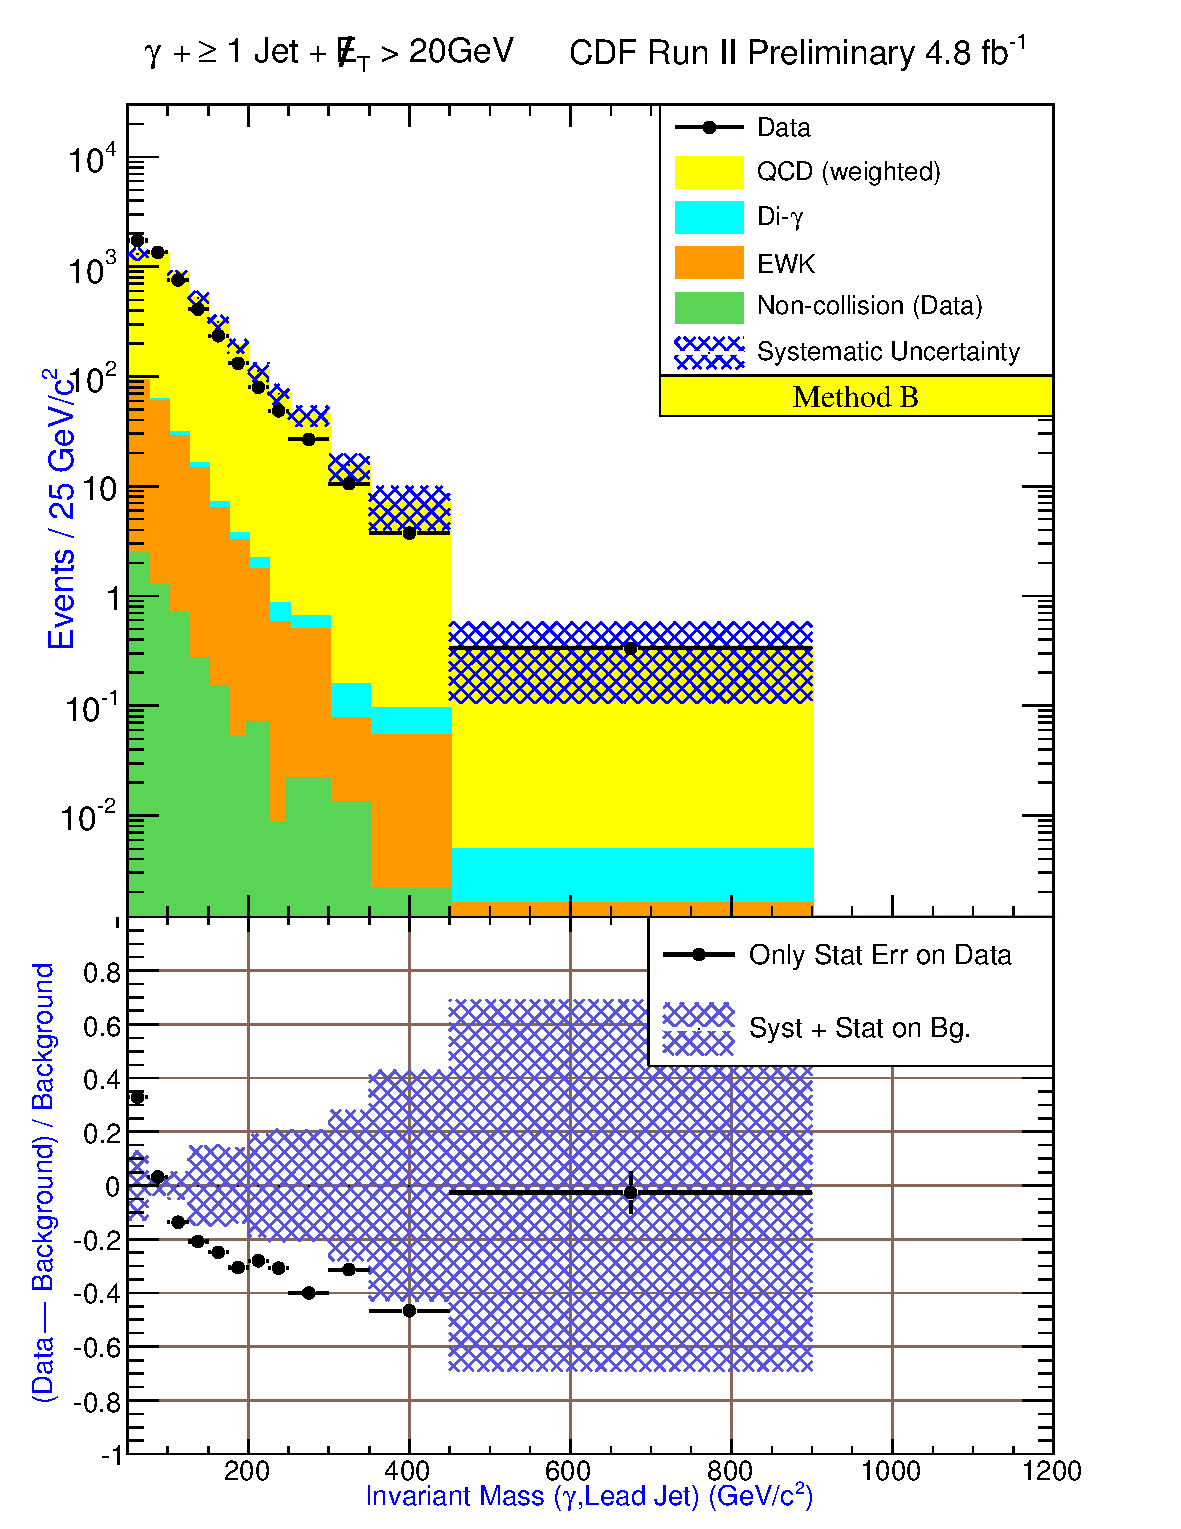
\includegraphics[keepaspectratio=true, scale=\figScale]{G30JetsMet20_MtdB_plot1_InvMass_pj1.pdf}}
\label{fig:pjmetMtdBSetOne}
\end{figure*}
\clearpage

\begin{figure*}[h!]
\centering
\caption[Method B \phoonejet]{Kinematic distributions of \phoonejet + \met$>$~20~GeV and \photwojet + \met$>$~20~GeV events using \mbox{Method B}. See Section~\ref{sec:PrelResults} for a description of the elements in these distributions.}
{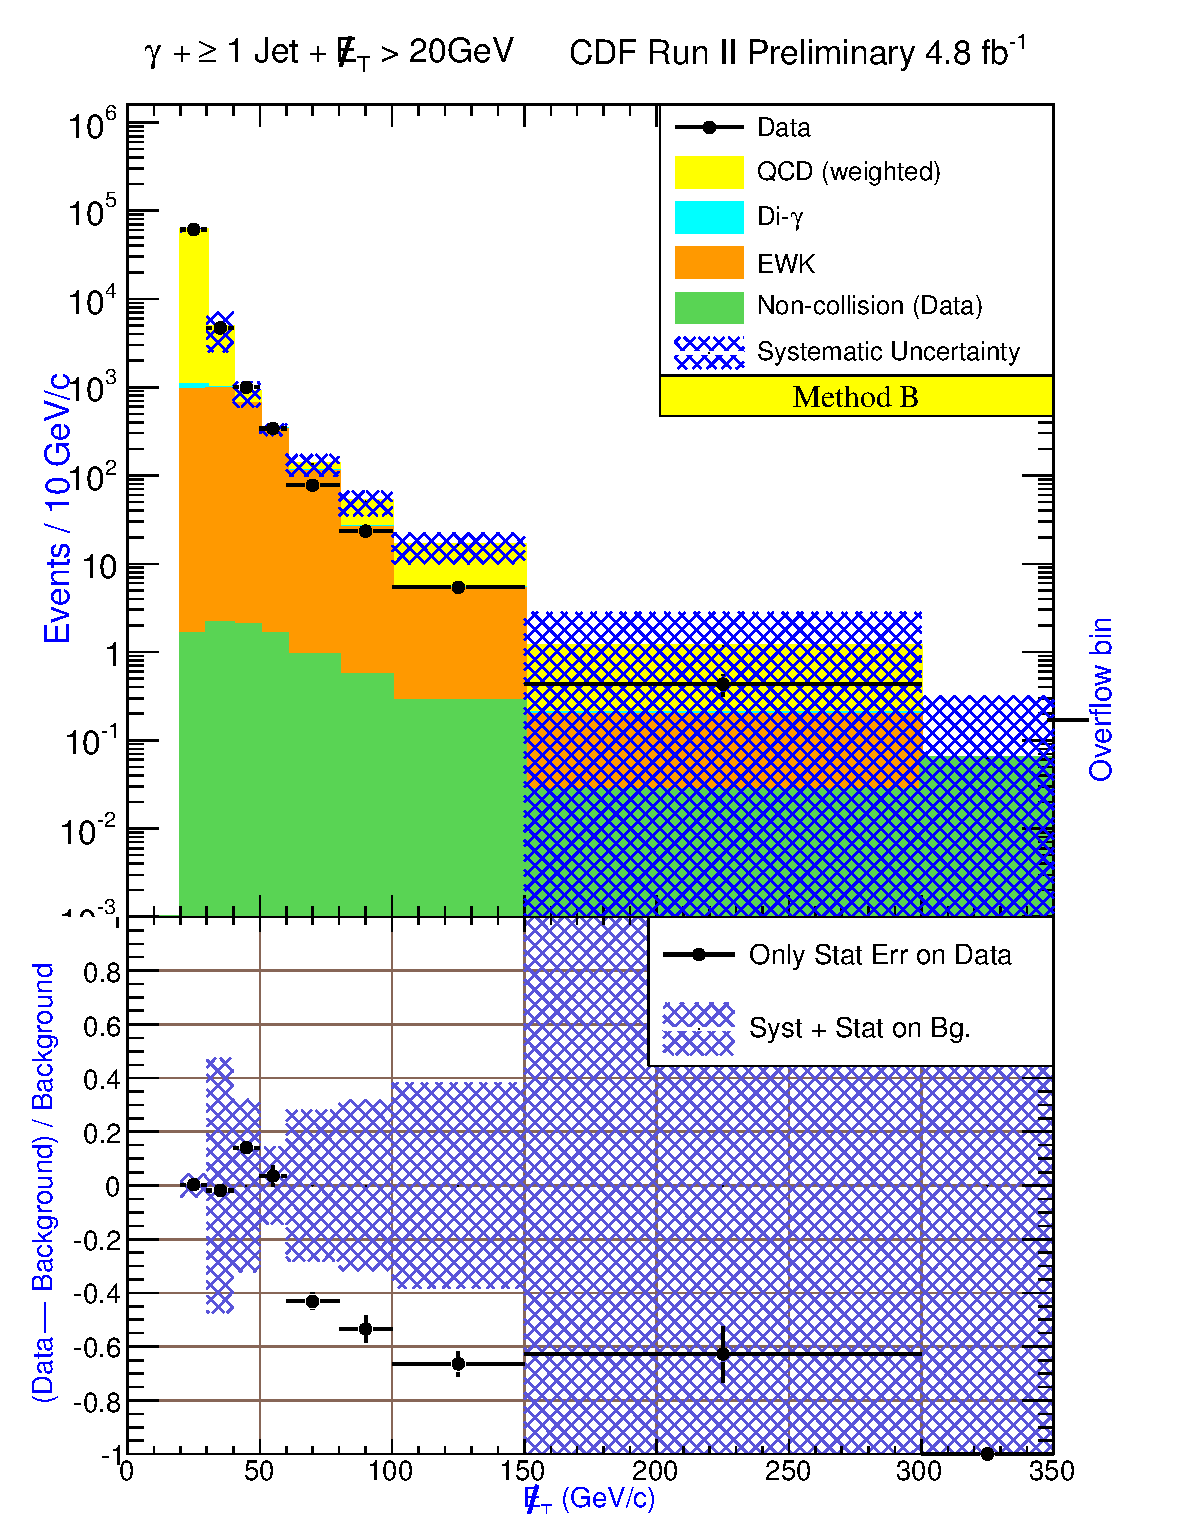
\includegraphics[keepaspectratio=true, scale=\figScale]{G30JetsMet20_MtdB_plot1_Met.pdf}}
{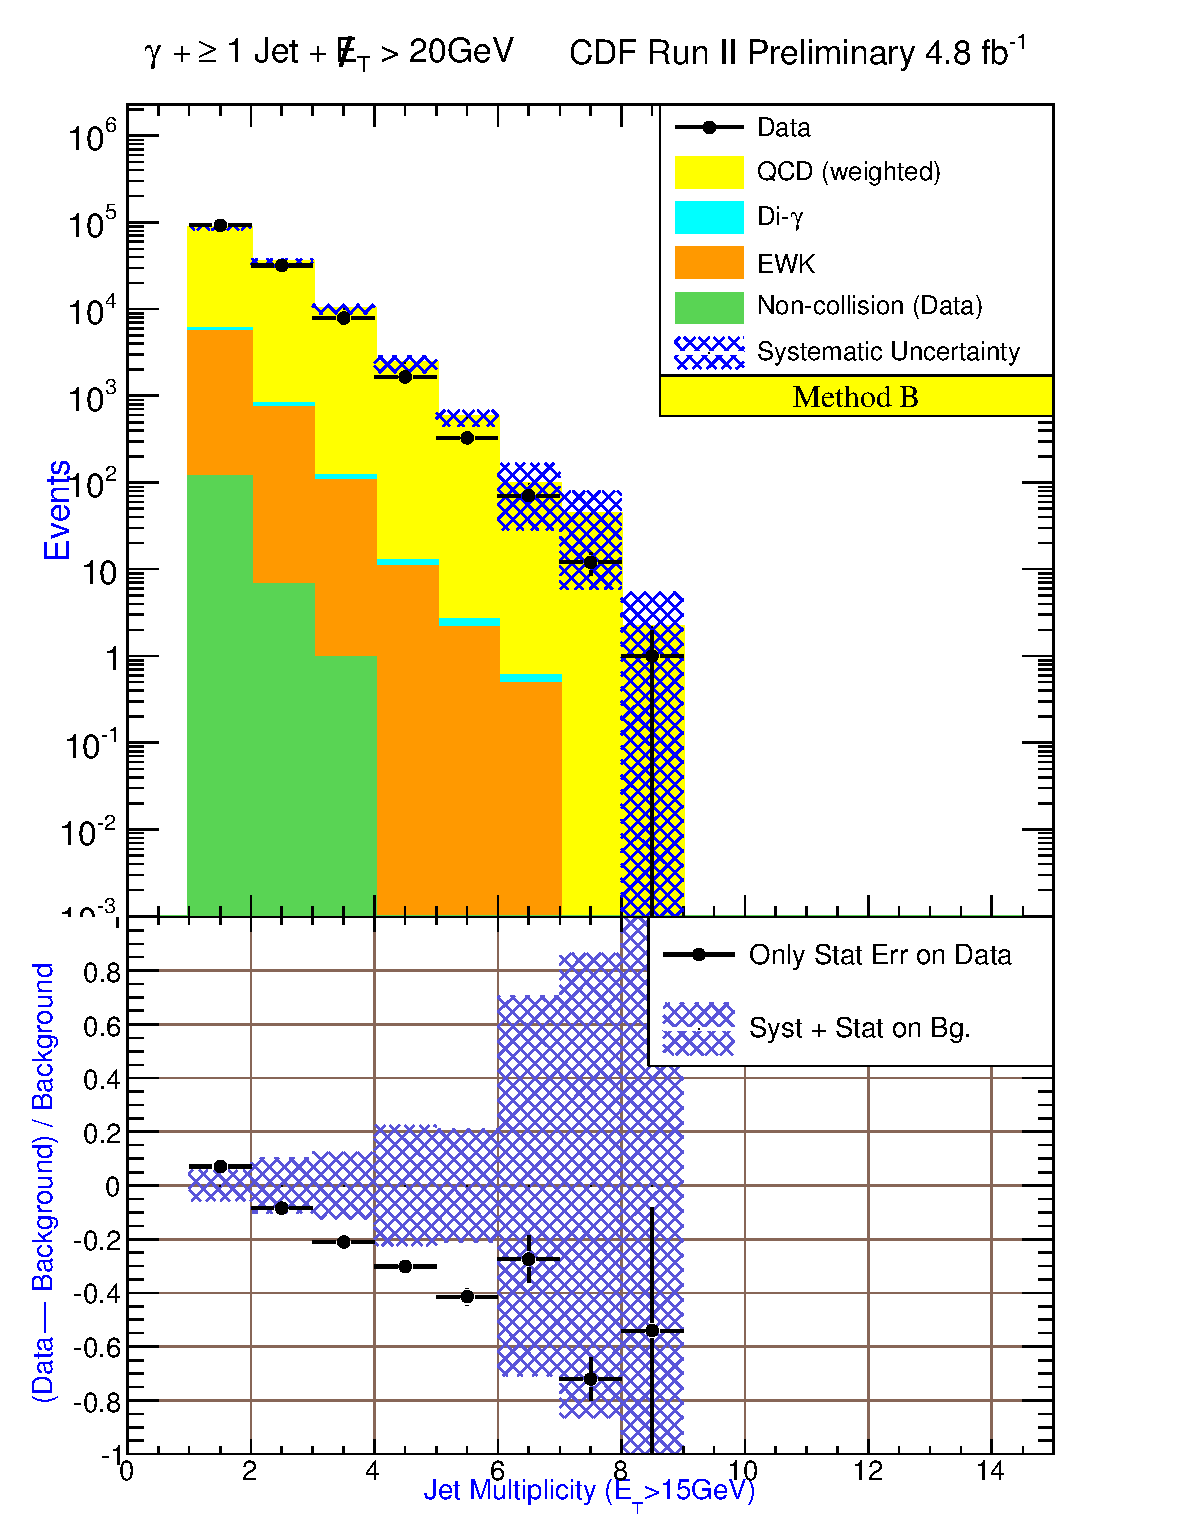
\includegraphics[keepaspectratio=true, scale=\figScale]{G30JetsMet20_MtdB_plot1_NJet.pdf}}
{\includegraphics[keepaspectratio=true, scale=\figScale]{G30JetsMet20_MtdB_plot2_Et_pho.pdf}}
{\includegraphics[keepaspectratio=true, scale=\figScale]{G30JetsMet20_MtdB_plot2_Et_j1.pdf}}
\label{fig:pjmetMtdBSetTwo}
\end{figure*}
\clearpage

\begin{figure*}[h!]
\centering
\caption[Method B \phoonejet]{Kinematic distributions of \photwojet + \met$>$~20~GeV events using \mbox{Method B}. See Section~\ref{sec:PrelResults} for a description of the elements in these distributions.}
{\includegraphics[keepaspectratio=true, scale=\figScale]{G30JetsMet20_MtdB_plot2_Ht.pdf}}
{\includegraphics[keepaspectratio=true, scale=\figScale]{G30JetsMet20_MtdB_plot2_InvMass_pj1.pdf}}
{\includegraphics[keepaspectratio=true, scale=\figScale]{G30JetsMet20_MtdB_plot2_InvMass_pj1j2.pdf}}
{\includegraphics[keepaspectratio=true, scale=\figScale]{G30JetsMet20_MtdB_plot2_InvMass_j1j2.pdf}}
\label{fig:pjmetMtdBSetThree}
\end{figure*}
\clearpage

\begin{figure*}[h!]
\centering
\caption[Method B \phoonejet]{Kinematic distributions of \photwojet + \met$>$~20~GeV events using \mbox{Method B}. See Section~\ref{sec:PrelResults} for a description of the elements in these distributions.}
{\includegraphics[keepaspectratio=true, scale=\figScale]{G30JetsMet20_MtdB_plot2_Met.pdf}}
\label{fig:pjmetMtdBSetFour}
\end{figure*}




\end{document}
%
% ****** End of file apssamp.tex ******
